\chapter{Méthodologie expérimentale et résultats}
\label{chap:resultats}

\section{Introduction}

Les chapitres précédents ont présenté l'architecture d'Ariel \logminer{} puis sa
traduction logicielle. Il reste à déterminer ce que cette architecture permet effectivement
d'observer lorsque ses différents mécanismes sont soumis à des expériences contrôlées.

L'évaluation d'un système de ce type ne peut pas se limiter à un score unique. Une bonne
performance de classification ne démontre pas que plusieurs formats de journaux sont
correctement normalisés. De même, une architecture distribuée fonctionnelle ne garantit
pas automatiquement un meilleur débit, et une tâche acquittée par un bus de messages
n'apporte pas la même preuve qu'une prédiction correctement classifiée.

La démarche expérimentale a donc été organisée autour de plusieurs objets distincts :
la généralisation des modèles supervisés, le comportement des méthodes appliquées aux
journaux système, la capacité de normalisation, le routage des sources, le coût de
l'architecture à agents, la distribution de tâches entre machines virtuelles, la
corrélation et la mise à jour contrôlée des modèles.

Un principe guide l'ensemble de ce chapitre : \textbf{chaque résultat est interprété dans
le périmètre exact du protocole qui l'a produit}. Un score élevé sur une séparation
aléatoire n'est pas utilisé comme preuve de généralisation à un scénario inédit. Une
anomalie candidate n'est pas assimilée à une attaque confirmée. Une validation multi-VM
de laboratoire n'est pas transformée en revendication de haute disponibilité industrielle.

Cette précaution conduit également à conserver les résultats négatifs. Plusieurs
expériences montrent en effet que certaines hypothèses intuitives ne sont pas confirmées :
la séparation par scénario dégrade fortement les performances sur CICIDS2017, les agents
n'améliorent pas le débit dans le benchmark contrôlé, certaines voies multiformat ne
normalisent aucune entrée et la spécialisation des modèles n'apporte pas un gain
prédictif systématique.

Ces observations constituent une partie importante de la contribution méthodologique du
travail.

\section{Principes généraux de l'évaluation}

\subsection{Séparation entre fonctionnalité et performance}

Deux niveaux de validation sont distingués.

Le premier est une \textbf{validation fonctionnelle}. Elle cherche à répondre à des
questions telles que :

\begin{itemize}
    \item le fichier est-il effectivement lu ?
    \item le parser produit-il une sortie ?
    \item une tâche Redis est-elle consommée ?
    \item un modèle candidat peut-il être promu ou rejeté ?
    \item le routeur retourne-t-il la famille attendue ?
\end{itemize}

Le second est une \textbf{évaluation quantitative}. Elle nécessite une vérité terrain ou
une mesure explicitement définie. Elle concerne par exemple :

\begin{itemize}
    \item le F1-score d'un classifieur ;
    \item le rappel ;
    \item le taux de faux positifs ;
    \item le débit en tâches par seconde ;
    \item la mémoire résidente ;
    \item la qualité du regroupement produit par le corrélateur.
\end{itemize}

Cette distinction évite d'utiliser une simple capture ou l'absence d'exception comme preuve
d'efficacité scientifique.

\subsection{Traçabilité des campagnes}

Les campagnes finales produisent des artefacts permettant de relier les valeurs utilisées
dans ce chapitre à leur exécution.

La chaîne de traçabilité suivie est de la forme :

\[
\text{résultat}
\longrightarrow
\text{run}
\longrightarrow
\text{configuration}
\longrightarrow
\text{script}
\longrightarrow
\text{données}.
\]

Un ledger append-only conserve les exécutions expérimentales importantes. Les résultats
bruts sont enregistrés dans des fichiers CSV ou JSON, puis agrégés pour les tableaux et
figures du mémoire.

Cette organisation réduit le risque de conserver dans la rédaction un ancien score après
modification du protocole.

\subsection{Résultats finaux et résultats exploratoires}

Seuls les protocoles finaux retenus sont utilisés comme base scientifique dans ce chapitre.

En particulier, pour HDFS et BGL, le protocole retenu ajuste Drain3 uniquement sur
l'ensemble d'entraînement puis gèle son état pour la validation et le test. Les anciens
résultats obtenus avec une préparation moins stricte ne sont pas utilisés pour conclure sur
la performance finale.

De même, aucun résultat de provenance insuffisamment établie n'est utilisé comme résultat
principal du mémoire.

\section{Environnement expérimental}

\subsection{Machine principale}

Les campagnes finales ont été exécutées principalement sous Windows 10, build 26200.

La machine dispose de :

\begin{itemize}
    \item 4 cœurs physiques ;
    \item 8 processeurs logiques ;
    \item environ 8,4~Go de mémoire vive disponible dans l'environnement documenté.
\end{itemize}

L'environnement Python principal est basé sur Python~3.11.9.

Le tableau~\ref{tab:env-final} reprend les versions logicielles les plus importantes
enregistrées dans le manifeste final.

\begin{table}[H]
\centering
\caption{Environnement logiciel principal des expériences finales}
\label{tab:env-final}
\small
\begin{tabular}{ll}
\toprule
\textbf{Composant} & \textbf{Version} \\
\midrule
Système principal & Windows 10, build 26200 \\
Python & 3.11.9 \\
scikit-learn & 1.7.2 \\
pandas & 2.3.2 \\
NumPy & 2.2.3 \\
SciPy & 1.16.1 \\
psutil & 7.2.2 \\
joblib & 1.5.2 \\
Client Python Redis & 8.0.1 \\
Drain3 & 0.9.11 \\
\bottomrule
\end{tabular}
\end{table}

Les versions exactes qui ne sont pas établies par les artefacts conservés ne sont pas
reconstituées a posteriori.

\subsection{Environnement multi-VM}

La validation multi-VM utilise un hôte Windows, VirtualBox ainsi que deux machines
virtuelles nommées Debian et Ubuntu.

Le service Redis de cette campagne est exécuté à partir de l'image
\texttt{redis:7-alpine}. Il est exposé sur le port 6379.

Depuis l'hôte, l'adresse utilisée est :

\begin{verbatim}
redis://localhost:6379/0
\end{verbatim}

Depuis les machines virtuelles configurées en NAT, le service est accessible à l'adresse :

\begin{verbatim}
redis://10.0.2.2:6379/0
\end{verbatim}

Cette topologie représente un environnement de laboratoire. Elle ne constitue pas une
infrastructure Redis répliquée ni un cluster hautement disponible.

\section{Sources de données}

\subsection{Catégories retenues}

Les sources utilisées dans le mémoire appartiennent à plusieurs catégories qu'il est
nécessaire de distinguer.

\begin{enumerate}
    \item \textbf{Datasets publics} : corpus distribués publiquement et décrits dans la
    littérature.

    \item \textbf{Collectes locales} : journaux provenant de systèmes ou postes utilisés
    dans le cadre du prototype.

    \item \textbf{Exports locaux} : données produites par un outil de supervision ou
    exportées depuis une plateforme locale.

    \item \textbf{Données synthétiques} : données construites volontairement pour tester
    un mécanisme précis avec une vérité connue.
\end{enumerate}

La catégorie d'une source ne détermine pas sa qualité. Elle détermine surtout la manière
dont sa provenance et ses limites doivent être décrites.

\subsection{Synthèse des sources}

Le tableau~\ref{tab:sources-experimentales} présente les principales sources exploitées.

\begin{table}[H]
\centering
\caption{Principales sources de données utilisées dans les expériences}
\label{tab:sources-experimentales}
\scriptsize
\begin{tabularx}{\textwidth}{p{2.6cm}p{2.6cm}p{3.1cm}X}
\toprule
\textbf{Source} &
\textbf{Catégorie} &
\textbf{Type} &
\textbf{Utilisation principale} \\
\midrule

CICIDS2017 &
Dataset public &
Flux réseau tabulaires labellisés &
Comparaison random/holdout et comparaison de cinq modèles supervisés. \\

HDFS &
Dataset public &
Journaux d'un système distribué &
Parsing Drain3 strict et détection d'anomalies sur fenêtres. \\

BGL &
Dataset public &
Journaux de supercalculateur &
Parsing Drain3 strict et détection d'anomalies. \\

Linux\_2k &
Dataset public &
Journaux Linux &
Validation fonctionnelle et corpus de routage lorsque utilisé. \\

Windows EVTX &
Collecte locale &
Événements Windows &
Validation multiformat et routage. \\

Linux/auth &
Source locale labellisée &
Événements d'authentification &
Pipeline et évaluations complémentaires. \\

Wazuh/Elastic &
Export local &
Événements de supervision enrichis &
Validation multiformat et routage. \\

Apache &
Fixture synthétique &
Journal d'accès web &
Cas limite de parsing/routage ; corpus très réduit. \\

Scénarios de corrélation &
Synthétique contrôlé &
19 événements &
Évaluation indépendante du regroupement d'incidents candidats. \\

\bottomrule
\end{tabularx}
\end{table}

CICIDS2017 est issu du Canadian Institute for Cybersecurity de l'Université du
Nouveau-Brunswick \cite{sharafaldin2018cicids}. HDFS et BGL sont des corpus de journaux
largement utilisés dans la littérature sur l'analyse automatique de logs
\cite{xu2009hdfs,oliner2007bgl,zhu2023loghub}.

Les expériences sont réalisées sur les copies locales présentes dans l'environnement
expérimental. Les hashes conservés dans les manifestes permettent d'identifier ces copies
et d'éviter qu'un changement silencieux du fichier ne passe inaperçu.

\section{Métriques de classification}

\subsection{Matrice de confusion}

Pour une classification binaire, quatre quantités structurent la majorité des métriques :

\begin{itemize}
    \item $TP$ : vrais positifs ;
    \item $TN$ : vrais négatifs ;
    \item $FP$ : faux positifs ;
    \item $FN$ : faux négatifs.
\end{itemize}

Un faux positif correspond à une observation normale classée comme positive. Un faux
négatif correspond à une observation positive non détectée.

Dans un contexte de cybersécurité, ces deux erreurs n'ont pas les mêmes conséquences.
Un nombre élevé de faux positifs augmente la charge d'analyse, tandis qu'un nombre élevé
de faux négatifs signifie que des événements appartenant à la classe recherchée passent
inaperçus.

\subsection{Exactitude}

L'exactitude, ou accuracy, est définie par :

\[
\mathrm{Accuracy}
=
\frac{TP + TN}
     {TP + TN + FP + FN}.
\]

Cette métrique est intuitive, mais elle peut être trompeuse lorsque les classes sont très
déséquilibrées.

\subsection{Précision}

La précision est définie par :

\[
\mathrm{Precision}
=
\frac{TP}{TP + FP}.
\]

Elle mesure la proportion de prédictions positives qui sont effectivement positives.

Une faible précision signifie qu'un analyste recevra de nombreux signaux injustifiés.

\subsection{Rappel}

Le rappel est donné par :

\[
\mathrm{Recall}
=
\frac{TP}{TP + FN}.
\]

Il mesure la fraction des observations positives effectivement retrouvées.

Un rappel faible est particulièrement problématique lorsque l'objectif principal est de
ne pas manquer certaines catégories d'événements.

\subsection{F1-score}

Le F1-score combine précision et rappel :

\[
F_1
=
2
\frac{\mathrm{Precision}\times\mathrm{Recall}}
{\mathrm{Precision}+\mathrm{Recall}}.
\]

Cette métrique devient particulièrement utile lorsqu'un compromis est nécessaire entre
faux positifs et faux négatifs.

\subsection{Taux de faux positifs}

Le taux de faux positifs est :

\[
\mathrm{FPR}
=
\frac{FP}{FP+TN}.
\]

Il renseigne sur la proportion d'observations négatives signalées à tort.

\subsection{Matthews Correlation Coefficient}

Le coefficient MCC est défini par :

\[
\mathrm{MCC}
=
\frac{TP\times TN-FP\times FN}
{\sqrt{(TP+FP)(TP+FN)(TN+FP)(TN+FN)}}.
\]

Il tient compte des quatre cases de la matrice de confusion et reste utile dans les
problèmes déséquilibrés.

\subsection{PR-AUC}

La PR-AUC représente l'aire sous la courbe précision--rappel lorsque le seuil de décision
varie.

Elle fournit une information différente d'un F1 calculé à un seuil unique. Un modèle peut,
par exemple, posséder une PR-AUC relativement élevée tout en obtenant un mauvais F1 au
seuil effectivement utilisé.

Cette distinction apparaît dans plusieurs résultats CICIDS2017.

\section{Protocole statistique}

Les expériences répétées n'utilisent pas toutes le même nombre d'exécutions.

Pour les méthodes stochastiques évaluées sur cinq seeds, les statistiques descriptives
comprennent notamment :

\begin{itemize}
    \item moyenne ;
    \item écart-type échantillonnal ;
    \item médiane ;
    \item minimum ;
    \item maximum.
\end{itemize}

Un intervalle de confiance à 95\,\% fondé sur Student est calculé uniquement lorsque
$N\geq2$ et lorsque cette statistique appartient effectivement aux artefacts de la
campagne.

Pour une méthode déterministe exécutée une seule fois, $N=1$. Aucun écart-type ni
intervalle de confiance ne doit alors être inventé.

Les comparaisons transversales restent essentiellement descriptives. Aucun test
inférentiel global n'est utilisé pour déclarer qu'un modèle est statistiquement supérieur
à tous les autres dans tous les scénarios.

\section{Expérience CICIDS2017 : sensibilité au protocole de séparation}

\subsection{Objectif}

La première expérience majeure cherche à répondre à une question méthodologique :
\textbf{dans quelle mesure la performance mesurée dépend-elle de la façon dont les données
sont séparées entre entraînement et test ?}

Deux protocoles sont comparés :

\begin{enumerate}
    \item une séparation aléatoire stratifiée ;
    \item un holdout dans lequel un scénario complet est exclu de l'entraînement.
\end{enumerate}

L'objectif n'est pas de désigner l'un des protocoles comme universellement correct.
La séparation aléatoire mesure la capacité à généraliser vers des observations provenant
de la même population mélangée. Le holdout par scénario impose une rupture plus forte et
renseigne davantage sur la capacité à traiter un contexte non présenté à l'entraînement.

\subsection{Scénarios}

Cinq scénarios sont successivement tenus hors entraînement :

\begin{itemize}
    \item DDoS ;
    \item PortScan ;
    \item Bot ;
    \item Infiltration ;
    \item WebAttacks.
\end{itemize}

Le label binaire utilisé est :

\[
\texttt{BENIGN}=0,
\qquad
\text{tout autre label}=1.
\]

\subsection{Caractéristiques}

Après exclusion des colonnes ne devant pas servir directement à la classification,
78 caractéristiques numériques sont retenues.

Les identifiants, adresses IP, timestamp, label et index sont exclus de l'entrée du modèle.

Les valeurs non finies sont remplacées par zéro et les valeurs extrêmes sont bornées dans
l'intervalle :

\[
[-10^{12},10^{12}].
\]

Ces choix sont appliqués de manière identique dans les protocoles comparés.

\subsection{Échantillonnage}

Pour les holdouts, le fichier ou scénario considéré est entièrement exclu du jeu
d'entraînement.

Le train est plafonné à :

\[
8\,000 \text{ observations par classe},
\]

et le test à :

\[
4\,000 \text{ observations par classe}.
\]

La lecture utilise au maximum deux chunks de 100\,000 lignes par fichier dans le protocole
retenu.

Pour le contrôle aléatoire, un pool fixe de 12\,000 lignes par classe est constitué avec
la seed 2026, puis séparé de manière stratifiée selon un rapport $2/3$--$1/3$ pour chacune
des seeds expérimentales.

\subsection{Seeds}

Les cinq seeds sont :

\[
42,\quad43,\quad44,\quad45,\quad46.
\]

Ce choix permet d'observer si la conclusion dépend fortement d'un seul tirage aléatoire.

\subsection{Random Forest}

Le modèle Random Forest est configuré avec :

\begin{itemize}
    \item 100 arbres ;
    \item profondeur maximale 28 ;
    \item \texttt{min\_samples\_leaf=2} ;
    \item \texttt{class\_weight=balanced} ;
    \item \texttt{n\_jobs=1}.
\end{itemize}

Aucun seuil n'est ajusté sur le jeu de test.

\subsection{Résultat du contrôle aléatoire}

Le Random Forest évalué avec le split aléatoire stratifié obtient :

\[
F_1
=
0{,}995142
\pm
0{,}001013.
\]

Pour $N=5$, l'intervalle de confiance à 95\,\% enregistré dans les statistiques finales est :

\[
[0{,}993884\,;\,0{,}996400].
\]

La faible dispersion entre seeds indique que, dans ce protocole aléatoire, la performance
est à la fois élevée et relativement stable.

Cette observation ne doit toutefois pas être interprétée comme une preuve de capacité à
traiter un scénario inédit.

\subsection{Résultat des holdouts}

Lorsque le test est constitué d'un scénario tenu hors entraînement, le F1 macro moyen tombe
à :

\[
F_{1,\mathrm{macro}}
=
0{,}157744.
\]

L'écart avec le contrôle aléatoire est considérable.

Le tableau~\ref{tab:cicids-holdout} présente les résultats structurants par scénario.

\begin{table}[H]
\centering
\caption{Résultats Random Forest des holdouts CICIDS2017}
\label{tab:cicids-holdout}
\small
\begin{tabularx}{\textwidth}{p{2.5cm}p{2.8cm}p{2.5cm}X}
\toprule
\textbf{Scénario tenu hors train} &
\textbf{F1} &
\textbf{Rappel} &
\textbf{Observation principale} \\
\midrule

DDoS &
$0{,}778774 \pm 0{,}001342$ &
$0{,}637700$ &
Seul scénario conservant une capacité de détection substantielle ; aucun faux positif en
moyenne dans le résumé final. \\

PortScan &
$0{,}009947$ &
$0{,}005000$ &
Très peu d'attaques sont classifiées positives malgré une PR-AUC de $0{,}881982$. \\

Bot &
$0$ &
$0$ &
Aucun vrai positif ; PR-AUC $0{,}322471$ sur 1\,966 attaques par test. \\

Infiltration &
$0$ &
$0$ &
Aucun vrai positif ; seulement 32 attaques dans le test correspondant. \\

WebAttacks &
$0$ &
$0$ &
Aucun vrai positif au seuil utilisé malgré une PR-AUC de $0{,}654341$. \\

\bottomrule
\end{tabularx}
\end{table}

La moyenne faible ne provient donc pas d'une dégradation uniforme. Elle résulte d'une
forte hétérogénéité entre scénarios.

DDoS conserve un F1 relativement élevé, alors que plusieurs scénarios aboutissent à un
F1 nul.

\subsection{Interprétation du cas PortScan}

Le cas PortScan est particulièrement instructif.

Son F1 est proche de zéro :

\[
F_1=0{,}009947,
\]

alors que la PR-AUC atteint :

\[
0{,}881982.
\]

Ces deux valeurs ne sont pas contradictoires.

La PR-AUC mesure le comportement obtenu lorsque le seuil varie. Le F1 correspond au point
de décision effectivement utilisé dans le protocole.

Le modèle semble donc conserver une information discriminante dans son score, mais le seuil
appliqué ne permet pas de transformer cette information en une détection satisfaisante du
scénario tenu hors entraînement.

Cette observation montre pourquoi il est dangereux de résumer un modèle par une seule
métrique.

\subsection{Interprétation des scénarios Bot et WebAttacks}

Pour Bot, aucun vrai positif n'est observé au seuil utilisé malgré la présence de
1\,966 attaques par test.

Le problème n'est donc pas simplement lié à l'absence d'exemples positifs dans le test.

WebAttacks présente également un F1 nul alors que sa PR-AUC atteint $0{,}654341$.

Une fois encore, le classement produit par les scores contient une information partielle,
mais celle-ci ne suffit pas à produire une classification positive correcte au seuil retenu.

\subsection{Infiltration}

Le scénario Infiltration contient seulement 32 observations positives dans le test.

Cette taille réduite impose une prudence supplémentaire : quelques prédictions modifient
fortement les métriques.

Le F1 nul reste un résultat réel du protocole, mais son interprétation ne doit pas être
séparée du faible nombre d'exemples positifs.

\subsection{Synthèse random versus holdout}

Le résultat central de cette expérience n'est pas que Random Forest est ``bon'' ou
``mauvais''.

Il est que :

\begin{quote}
\textit{la conclusion change profondément lorsque le protocole de séparation change.}
\end{quote}

Un F1 proche de 1 sur un split aléatoire coexiste avec un F1 macro d'environ 0,158 lorsque
le test est construit autour de scénarios exclus de l'apprentissage.

La campagne multi-seeds montre que cette différence ne peut pas être réduite à une seed
particulière.

\IfFileExists{figures/cicids_random_vs_holdout_f1.png}{
\begin{figure}[H]
\centering

\includegraphics[width=0.82\textwidth]{figures/cicids_random_vs_holdout_f1.png}
\caption{Comparaison du F1 entre contrôle aléatoire et holdouts CICIDS2017.}
\label{fig:cicids-random-holdout}
\end{figure}

\begin{center}
\footnotesize Source : auteur, à partir des résultats expérimentaux de ce travail.
\end{center}
}{}

\IfFileExists{figures/cicids_f1_scenario_seed_heatmap.png}{
\begin{figure}[H]
\centering

\includegraphics[width=0.88\textwidth]{figures/cicids_f1_scenario_seed_heatmap.png}
\caption{Variation du F1 selon le scénario CICIDS2017 tenu hors entraînement et la seed.}
\label{fig:cicids-heatmap}
\end{figure}

\begin{center}
\footnotesize Source : auteur, à partir des résultats expérimentaux de ce travail.
\end{center}
}{}

\begin{figure}[H]
\centering
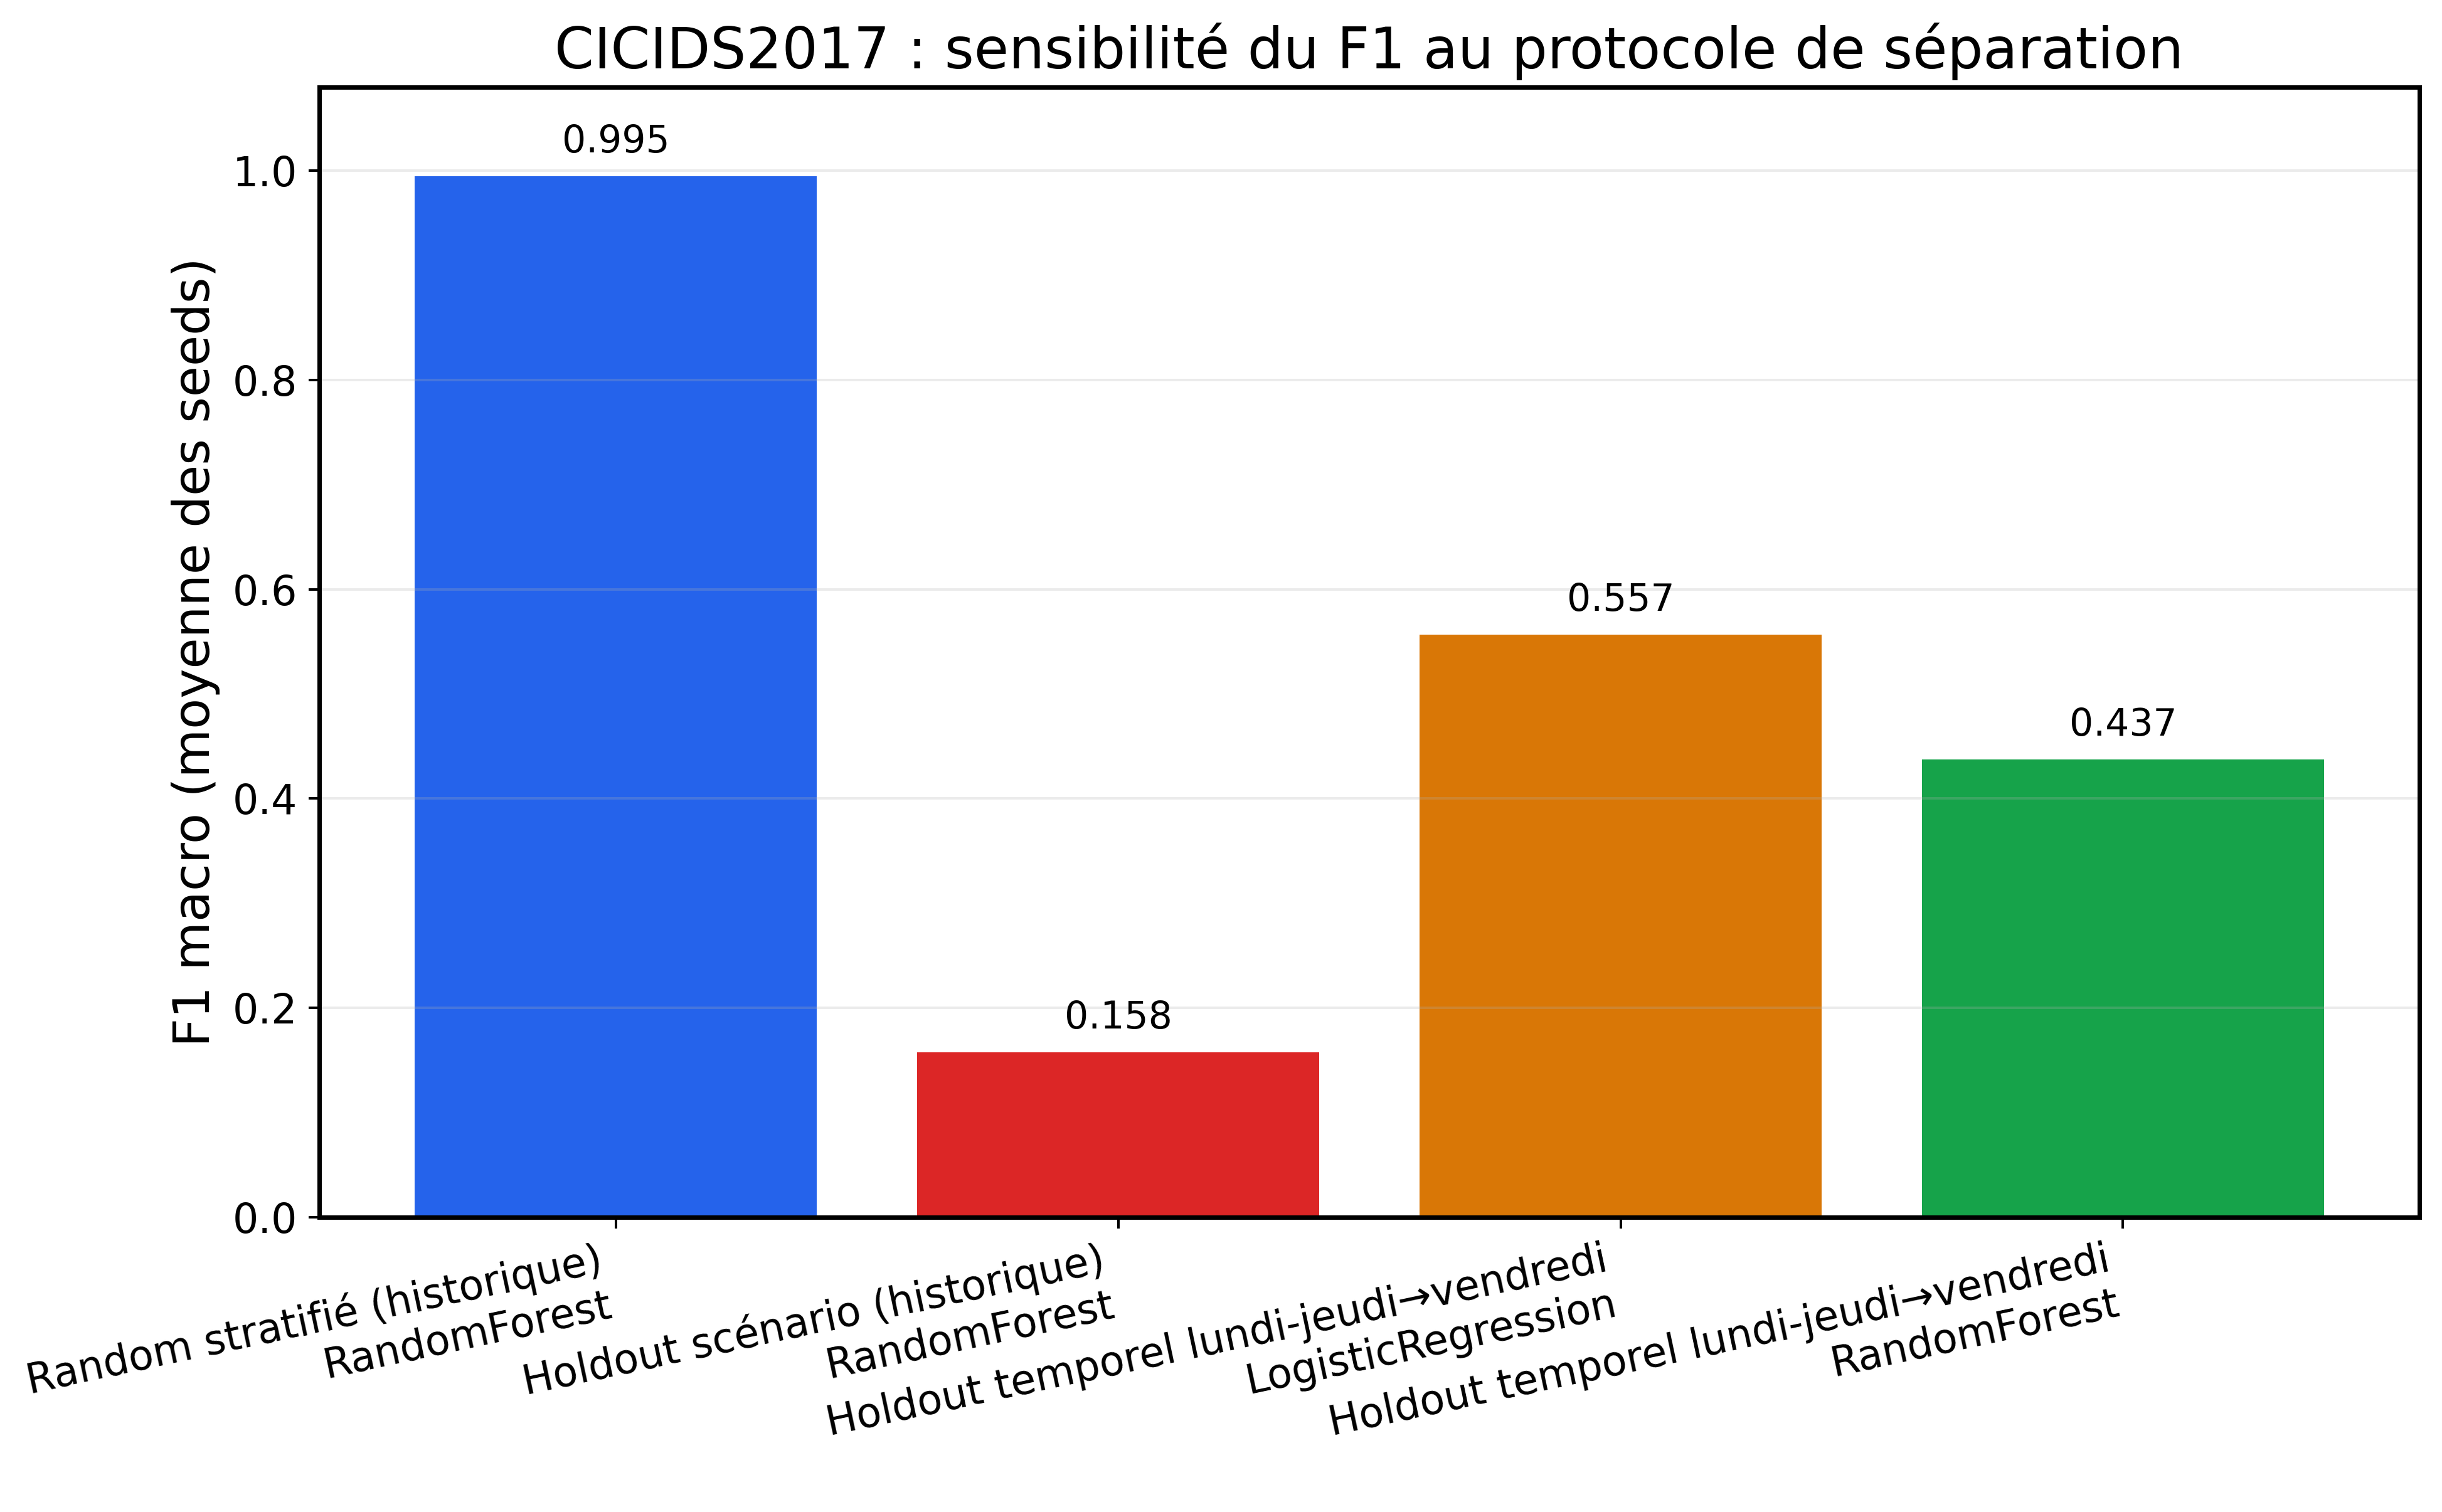
\includegraphics[width=0.96\textwidth]{figures/final/fig_cicids_protocol_comparison.png}
\caption{Comparaison des protocoles CICIDS2017 à partir des cinq seeds disponibles.
La séparation aléatoire et les holdouts ne mesurent pas la même capacité de généralisation ;
la figure soutient l'interprétation méthodologique du chapitre.}
\label{fig:cicids-protocol-comparison-final}
\end{figure}

\section{Comparaison de cinq modèles sur les holdouts CICIDS2017}

\subsection{Objectif}

La chute observée avec Random Forest peut provenir soit du protocole lui-même, soit d'un
mauvais choix d'algorithme.

Une seconde campagne compare donc cinq modèles dans les mêmes conditions de holdout.

Les candidats sont :

\begin{enumerate}
    \item Random Forest ;
    \item Extra Trees ;
    \item HistGradientBoosting ;
    \item Logistic Regression ;
    \item SGDClassifier à perte logistique.
\end{enumerate}

\subsection{Protocole}

La campagne conserve :

\begin{itemize}
    \item les cinq scénarios précédents ;
    \item les seeds 42 à 46 ;
    \item les mêmes règles d'échantillonnage ;
    \item les mêmes caractéristiques.
\end{itemize}

Cela représente :

\[
5 \text{ modèles}
\times
5 \text{ scénarios}
\times
5 \text{ seeds}
=
125 \text{ exécutions}.
\]

Les deux modèles linéaires utilisent un \texttt{StandardScaler} ajusté exclusivement sur
le train.

Le scaler n'est donc jamais estimé à partir du test.

Les métriques enregistrées comprennent :

\begin{itemize}
    \item précision ;
    \item rappel ;
    \item F1 ;
    \item PR-AUC ;
    \item MCC ;
    \item FPR ;
    \item matrice de confusion ;
    \item temps d'exécution.
\end{itemize}

\subsection{Meilleur F1 macro}

Logistic Regression obtient le meilleur F1 macro parmi les cinq candidats :

\[
F_{1,\mathrm{macro}}=0{,}233670.
\]

Son MCC macro est :

\[
MCC=0{,}186858.
\]

Ce résultat améliore le F1 macro observé avec Random Forest, mais il reste faible au regard
de la performance obtenue avec le split aléatoire.

Le changement d'algorithme ne supprime donc pas la fragilité inter-scénarios.

\subsection{PR-AUC}

HistGradientBoosting obtient la meilleure PR-AUC macro parmi les candidats documentés :

\[
\mathrm{PR\mbox{-}AUC}_{\mathrm{macro}}
=
0{,}567697.
\]

Cette différence montre qu'il n'existe pas un modèle dominant selon toutes les métriques.

Logistic Regression est le meilleur selon le F1 macro du protocole, mais cette observation
ne permet pas d'affirmer qu'il est universellement le meilleur modèle.

\subsection{Échec persistant sur Bot}

Un résultat particulièrement important est que les cinq modèles ne résolvent pas le
scénario Bot dans les conditions strictes retenues.

Changer d'algorithme ne suffit donc pas à corriger toutes les difficultés de
généralisation.

Cette observation suggère que le problème peut concerner davantage :

\begin{itemize}
    \item la représentation ;
    \item le déplacement de distribution ;
    \item la spécificité du scénario ;
    \item ou l'information réellement disponible dans les caractéristiques.
\end{itemize}

Il serait donc peu justifié de répondre à cet échec uniquement en ajoutant un sixième
classifieur sans examiner les données.

\IfFileExists{figures/cicids_modeles_scenarios_f1.png}{
\begin{figure}[H]
\centering

\includegraphics[width=0.90\textwidth]{figures/cicids_modeles_scenarios_f1.png}
\caption{F1 des cinq modèles selon les scénarios CICIDS2017 tenus hors entraînement.}
\label{fig:cicids-modeles}
\end{figure}

\begin{center}
\footnotesize Source : auteur, à partir des résultats expérimentaux de ce travail.
\end{center}
}{}

\begin{figure}[H]
\centering
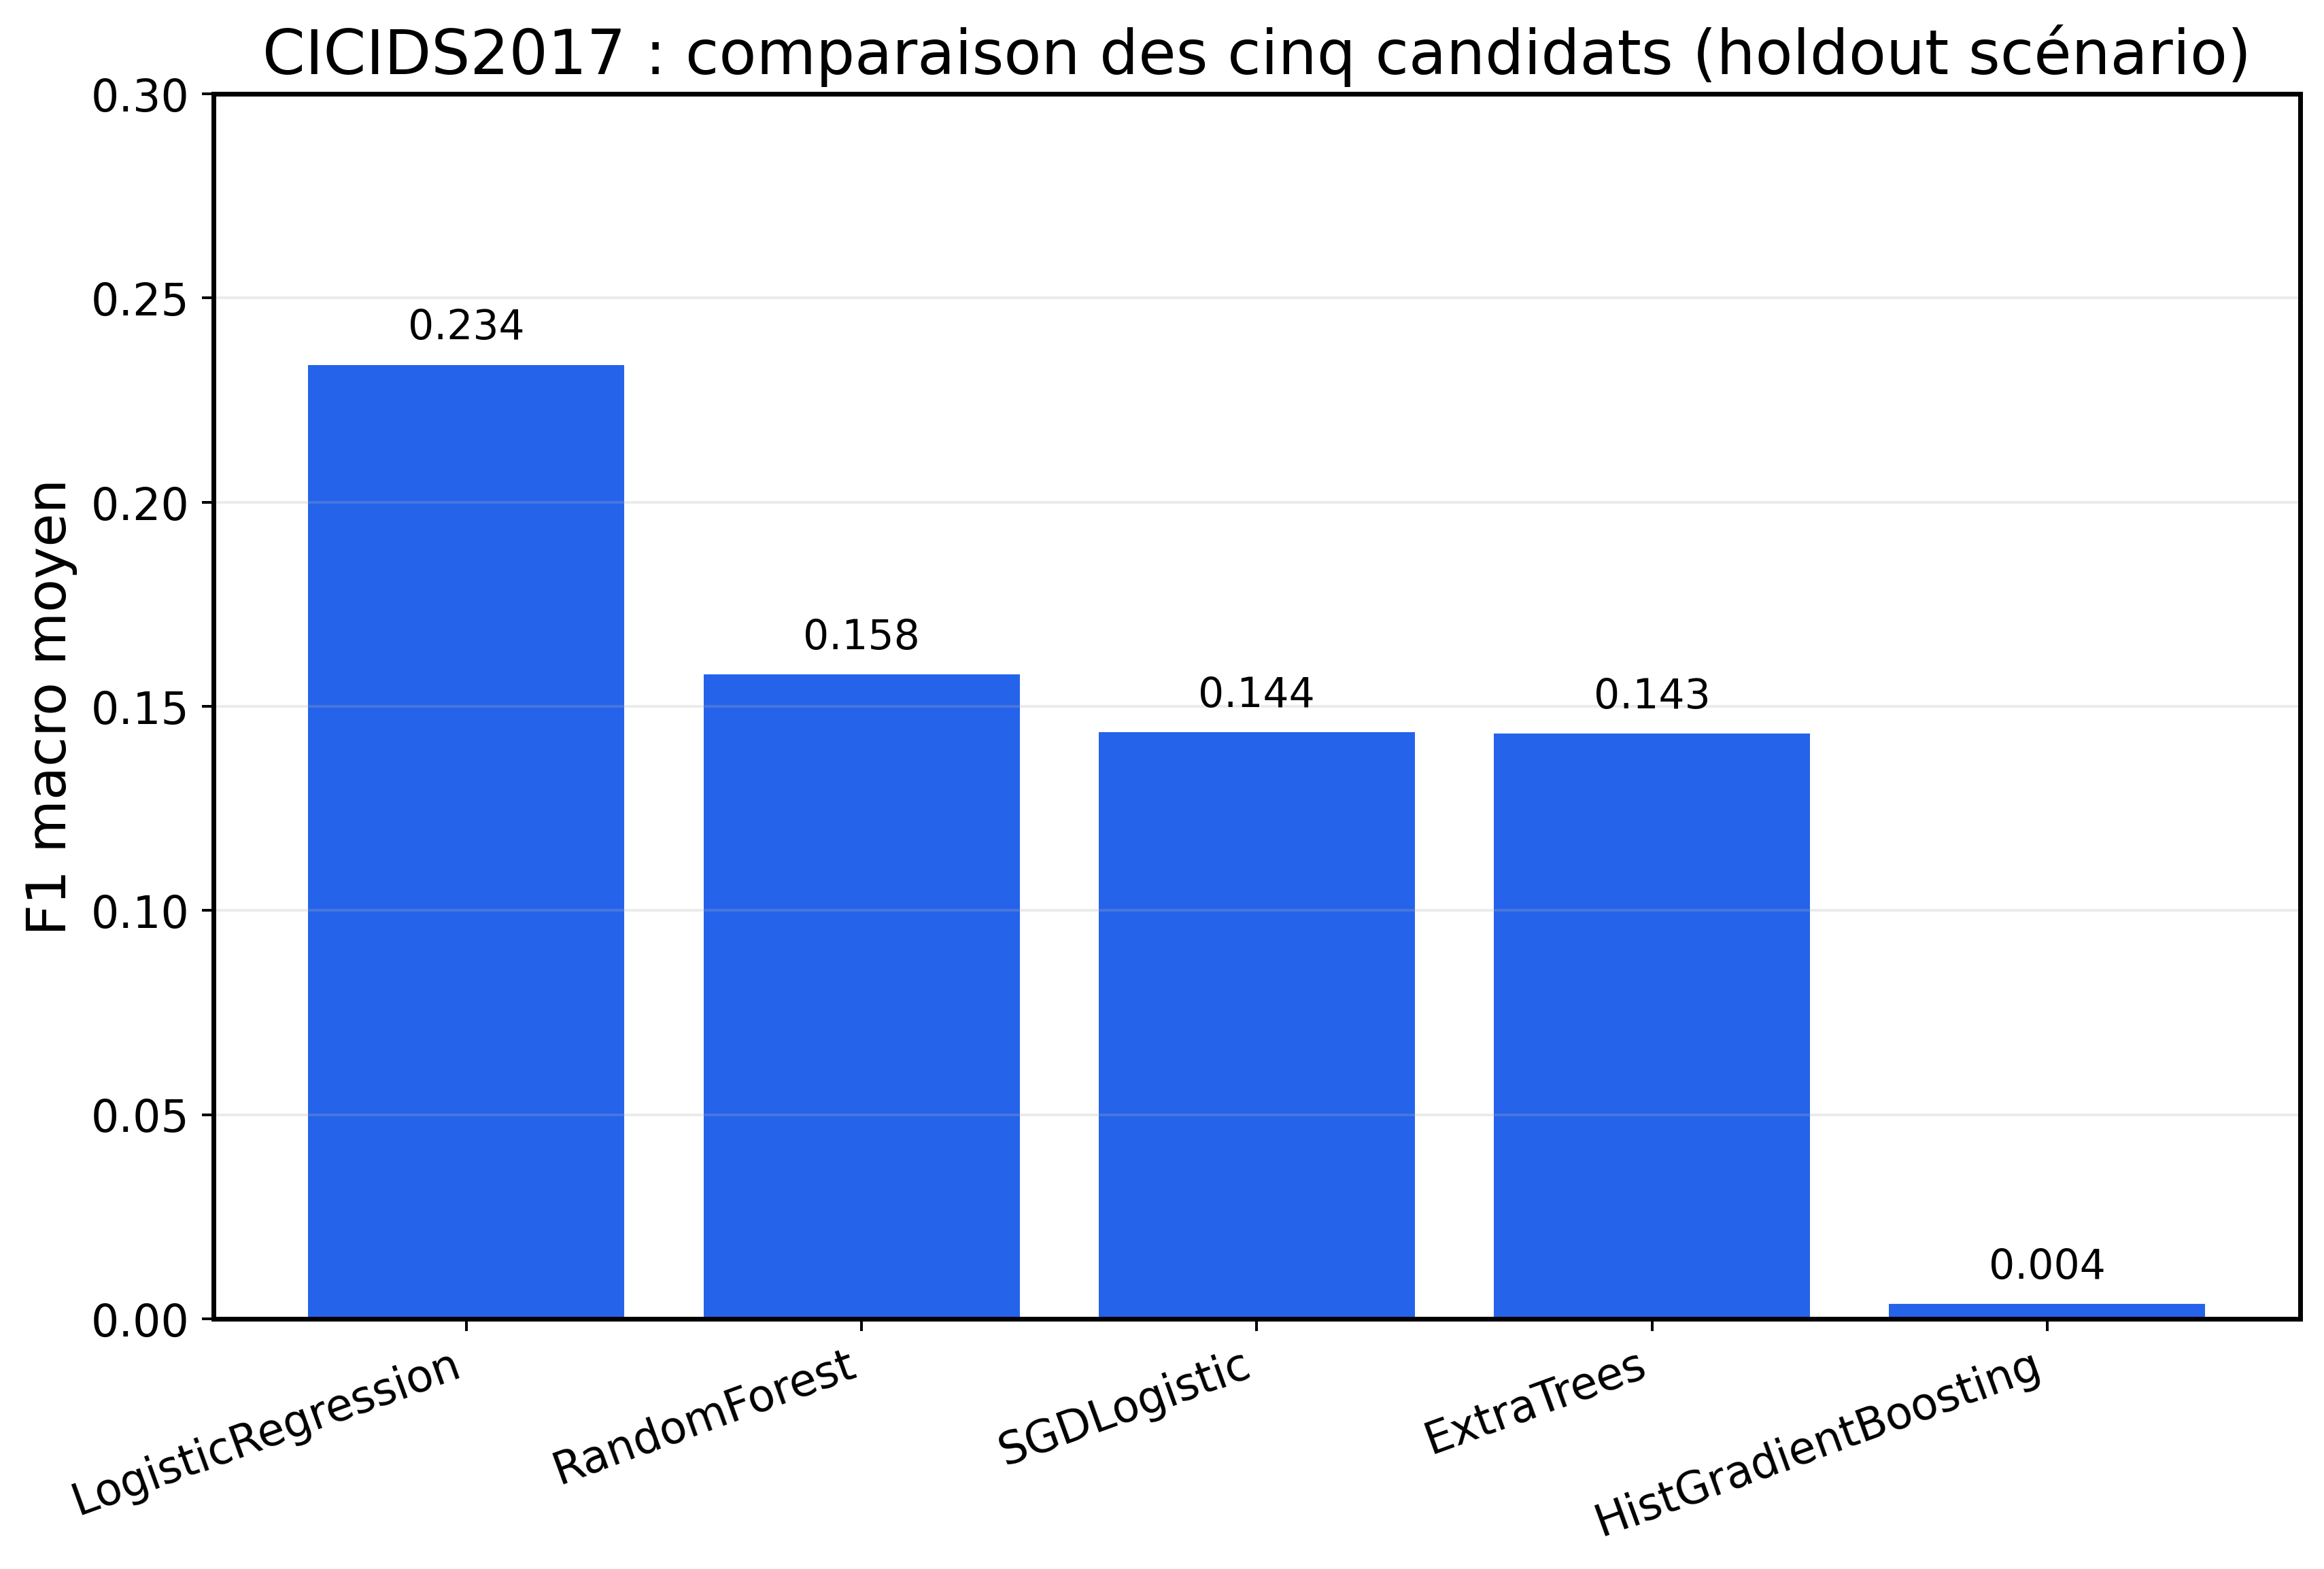
\includegraphics[width=0.92\textwidth]{figures/final/fig_cicids_model_comparison.png}
\caption{Comparaison des cinq candidats CICIDS2017 sur le holdout par scénario.
Les valeurs sont les moyennes des cinq seeds ; la figure permet de distinguer le meilleur
F1 macro du meilleur PR-AUC macro.}
\label{fig:cicids-model-comparison-final}
\end{figure}

\subsection{Conclusion de la comparaison}

La comparaison de modèles apporte deux enseignements.

Premièrement, le choix du modèle possède un effet réel : Logistic Regression améliore le
F1 macro et HistGradientBoosting obtient une PR-AUC macro supérieure.

Deuxièmement, aucun des candidats ne supprime le contraste observé entre les scénarios.

La difficulté principale n'est donc pas uniquement le choix d'un algorithme. La
construction du test et la différence entre les scénarios jouent un rôle central.

\section{Protocole strict HDFS/BGL}

\subsection{Motivation}

Les journaux HDFS et BGL diffèrent fortement de CICIDS2017.

Ils ne sont pas représentés à l'origine comme un tableau de flux réseau composé de dizaines
de caractéristiques numériques. Le message lui-même, sa structure et son contexte
temporel jouent un rôle important.

L'objectif est donc de construire un protocole dans lequel les représentations utilisées
pour le test ne profitent pas d'informations apprises sur ce même test.

\subsection{Partition chronologique}

Les données sont séparées selon trois plages disjointes :

\[
\text{Train}=0\text{--}60\,\%,
\]

\[
\text{Validation}=60\text{--}80\,\%,
\]

\[
\text{Test}=80\text{--}100\,\%.
\]

Les échantillons sont prélevés autour des positions relatives $0,3$, $0,7$ et $0,9$.

Les volumes cibles avant filtrage sont :

\[
50\,000/20\,000/20\,000.
\]

Pour HDFS, les volumes effectivement utilisés sont :

\begin{itemize}
    \item Train : 50\,000 ;
    \item Validation : 20\,000 ;
    \item Test : 20\,000.
\end{itemize}

Après la déduplication inter-partitions, aucun \texttt{block\_id} n'est partagé entre les
partitions.

Pour BGL, les volumes observés sont :

\begin{itemize}
    \item Train : 49\,999 ;
    \item Validation : 17\,764 ;
    \item Test : 19\,908.
\end{itemize}

La sélection des plages est réalisée sans utiliser les labels.

\subsection{Drain3 train-only}

Drain3 version 0.9.11 est ajusté uniquement sur le train.

La configuration principale utilise :

\begin{itemize}
    \item \texttt{sim\_th=0.4} ;
    \item profondeur 4 ;
    \item maximum de 100 enfants ;
    \item paramétrisation des nombres.
\end{itemize}

Après cette étape, l'état du parseur est gelé.

Pour la validation et le test, les messages sont uniquement comparés aux clusters existants
au moyen de la stratégie de matching prévue.

Aucun appel d'apprentissage de nouveaux templates n'est effectué sur la validation ou le
test.

Ce choix évite qu'un template observé pour la première fois dans le test soit incorporé au
modèle avant sa propre évaluation.

\subsection{Fenêtres}

Les événements sont organisés dans des fenêtres passées de 30 minutes.

L'état des fenêtres est réinitialisé à chaque partition.

Les statistiques de fréquence par template et par source sont calculées uniquement à
partir du train.

Lorsqu'un scaler est nécessaire, il est ajusté uniquement sur les observations normales
du train.

\subsection{Choix du seuil}

Le seuil est sélectionné sur la validation.

Le critère principal est le F1 maximal.

En cas d'égalité, les départages sont appliqués selon :

\begin{enumerate}
    \item FPR minimal ;
    \item MCC maximal ;
    \item seuil maximal.
\end{enumerate}

Aucune information sur la prévalence ou la distribution du test n'est utilisée pour choisir
le seuil.

\subsection{Méthodes}

Les méthodes évaluées comprennent :

\begin{itemize}
    \item Isolation Forest ;
    \item Z-score ;
    \item IQR ;
    \item Histogram ;
    \item AutoencoderMLP ;
    \item ensemble calibré sur le train.
\end{itemize}

Les méthodes stochastiques utilisent les seeds 42 à 46.

Les méthodes déterministes sont évaluées avec :

\[
N=1.
\]

\section{Résultats HDFS au niveau bloc}

La granularité principale retenue pour HDFS est désormais \texttt{block\_id}, c'est-à-dire l'unité
sur laquelle la vérité terrain est définie. Le parseur Drain3 est ajusté sur le train puis
gelé ; les partitions de validation et de test utilisent uniquement un appariement aux
templates existants. L'agrégateur est la moyenne des scores d'événements d'un bloc et le
seuil est choisi sur la validation :

\[
\tau_{\mathrm{val}}=1.2729429339548877.
\]

Sur le test gelé de 2\,000 blocs, dont 29 positifs, Histogram obtient :

\[
F_1=0{,}892308,
\qquad TP=29,\ FP=7,\ TN=1964,\ FN=0.
\]

Le rappel vaut donc 1 dans ce test, mais le faible nombre de blocs positifs impose une
lecture prudente. Un bootstrap descriptif de 1\,000 réplications par \texttt{block\_id} donne une
médiane de F1 de $0{,}894737$ et un intervalle percentile
$[0{,}800000\,;\,0{,}961039]$. Les 29 retraits d'un bloc positif donnent tous un F1 de
$0{,}888889$ ; cette stabilité du rappel ne supprime pas la variabilité globale. Le F1
observé au niveau bloc vaut donc $0{,}892308$ sur le test gelé, tandis que l'analyse
bootstrap met en évidence une variabilité non négligeable liée notamment au faible nombre
de blocs positifs.

\begin{figure}[H]
\centering
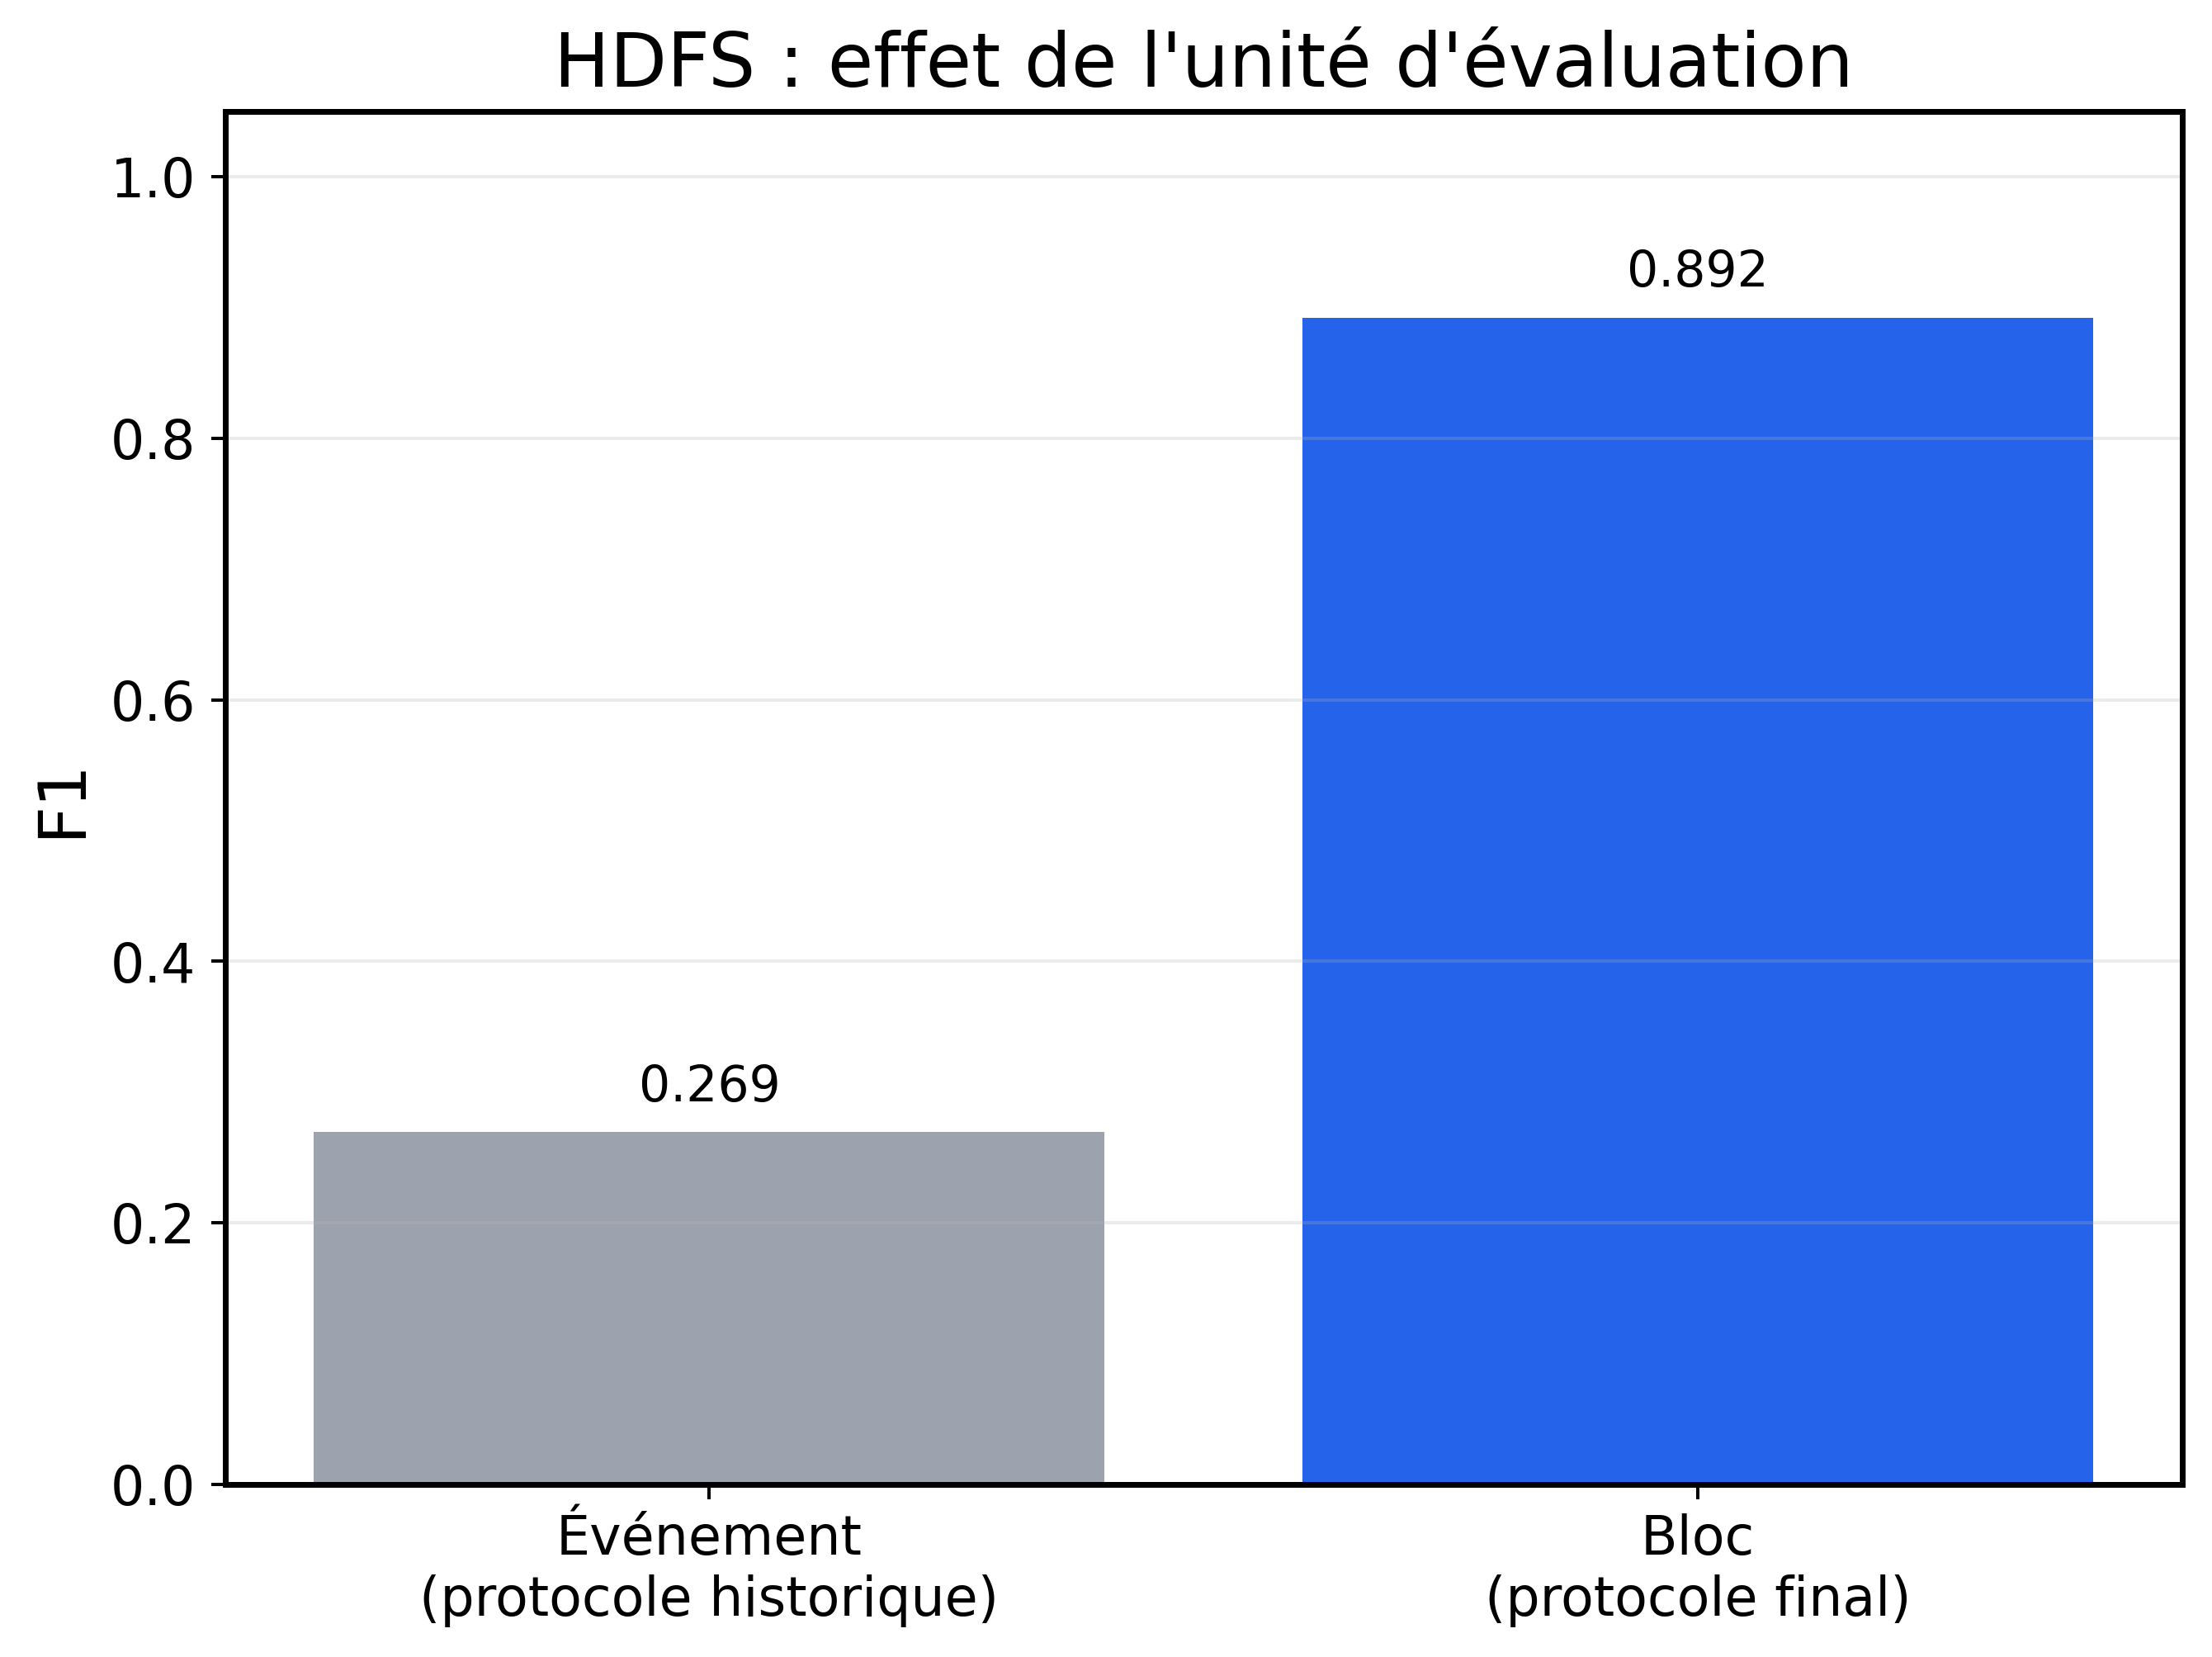
\includegraphics[width=0.78\textwidth]{figures/final/fig_hdfs_event_vs_block.png}
\caption{HDFS : comparaison entre l'ancien protocole événementiel et le protocole final au
niveau bloc. La valeur historique n'est pas un benchmark équivalent ; le niveau bloc est
aligné sur la définition de la vérité terrain.}
\label{fig:hdfs-event-block-final}
\end{figure}

\begin{figure}[H]
\centering
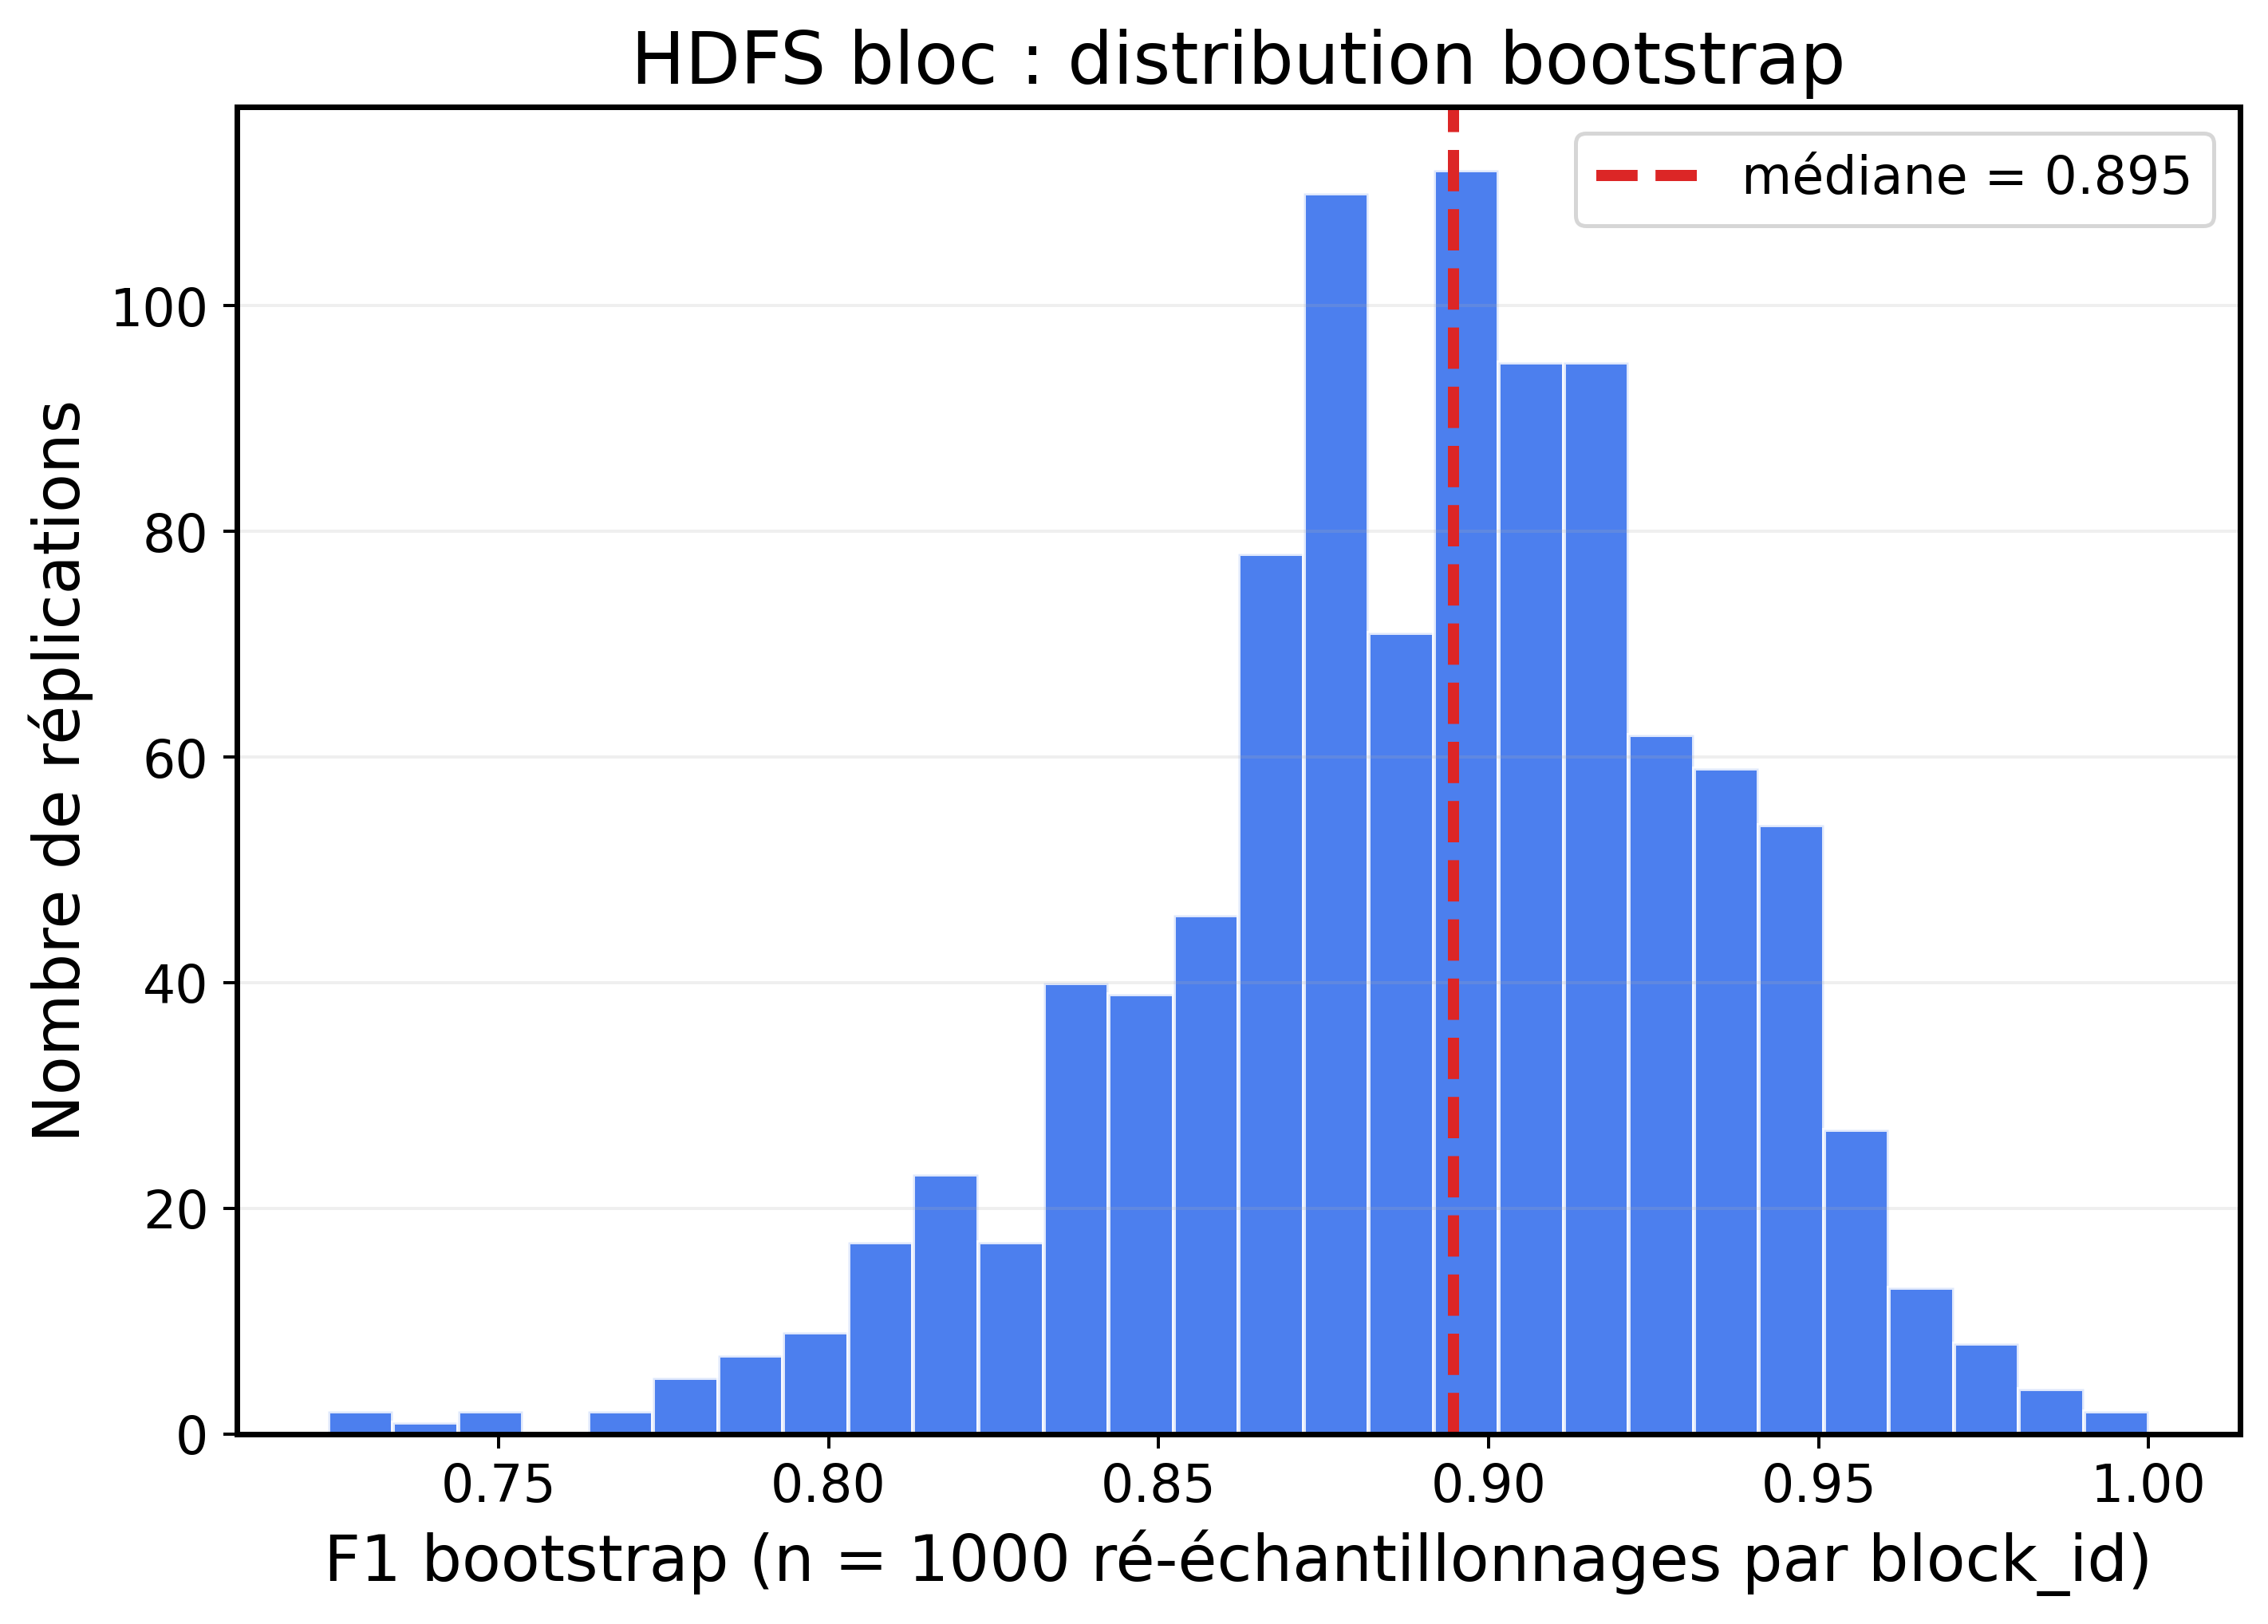
\includegraphics[width=0.82\textwidth]{figures/final/fig_hdfs_bootstrap_distribution.png}
\caption{Distribution bootstrap du F1 HDFS au niveau bloc (1\,000 réplications par
\texttt{block\_id}). La médiane et l'intervalle empirique rendent visible l'incertitude
associée au faible nombre de blocs positifs.}
\label{fig:hdfs-bootstrap-final}
\end{figure}

\subsection{Particularité des labels HDFS}

La réagrégation au niveau \texttt{block\_id} évite d'interpréter chaque événement d'un bloc
anormal comme une anomalie indépendante. Les statistiques rapportées sont descriptives et
ne constituent pas une preuve d'indépendance entre blocs ni une généralisation à tous les
journaux HDFS.

\section{Résultats BGL}

Sur BGL, Histogram obtient :

\[
F_1=0{,}913698.
\]

Le taux de faux positifs est :

\[
FPR=0{,}032016.
\]

Ce résultat est nettement supérieur à celui de HDFS dans le même cadre méthodologique.

Il ne permet cependant pas de conclure que BGL est intrinsèquement un problème simple.

Deux particularités doivent être conservées dans l'interprétation :

\begin{itemize}
    \item le train ne contient pas d'anomalies dans la configuration retenue ;
    \item environ 89,808\,\% des templates du test sont inconnus par rapport à l'état appris
    sur le train.
\end{itemize}

Le comportement du détecteur dépend donc fortement du déplacement de distribution et de la
manière dont la nouveauté des templates est représentée.

Une baseline qui déclare toute observation dont le template est inconnu comme anomalie
obtient seulement un F1 de $0{,}277885$. Le F1 de Histogram ne peut donc pas être expliqué
par la seule nouveauté des templates. Toutefois, tous les vrais positifs observés se
trouvent dans le groupe \texttt{UNKNOWN\_TEMPLATE} et le groupe \texttt{KNOWN\_TEMPLATE} ne contient
aucune anomalie dans cette partition. Le rappel sur des anomalies à template connu reste
donc \textbf{INFORMATION À VÉRIFIER}.

\begin{figure}[H]
\centering
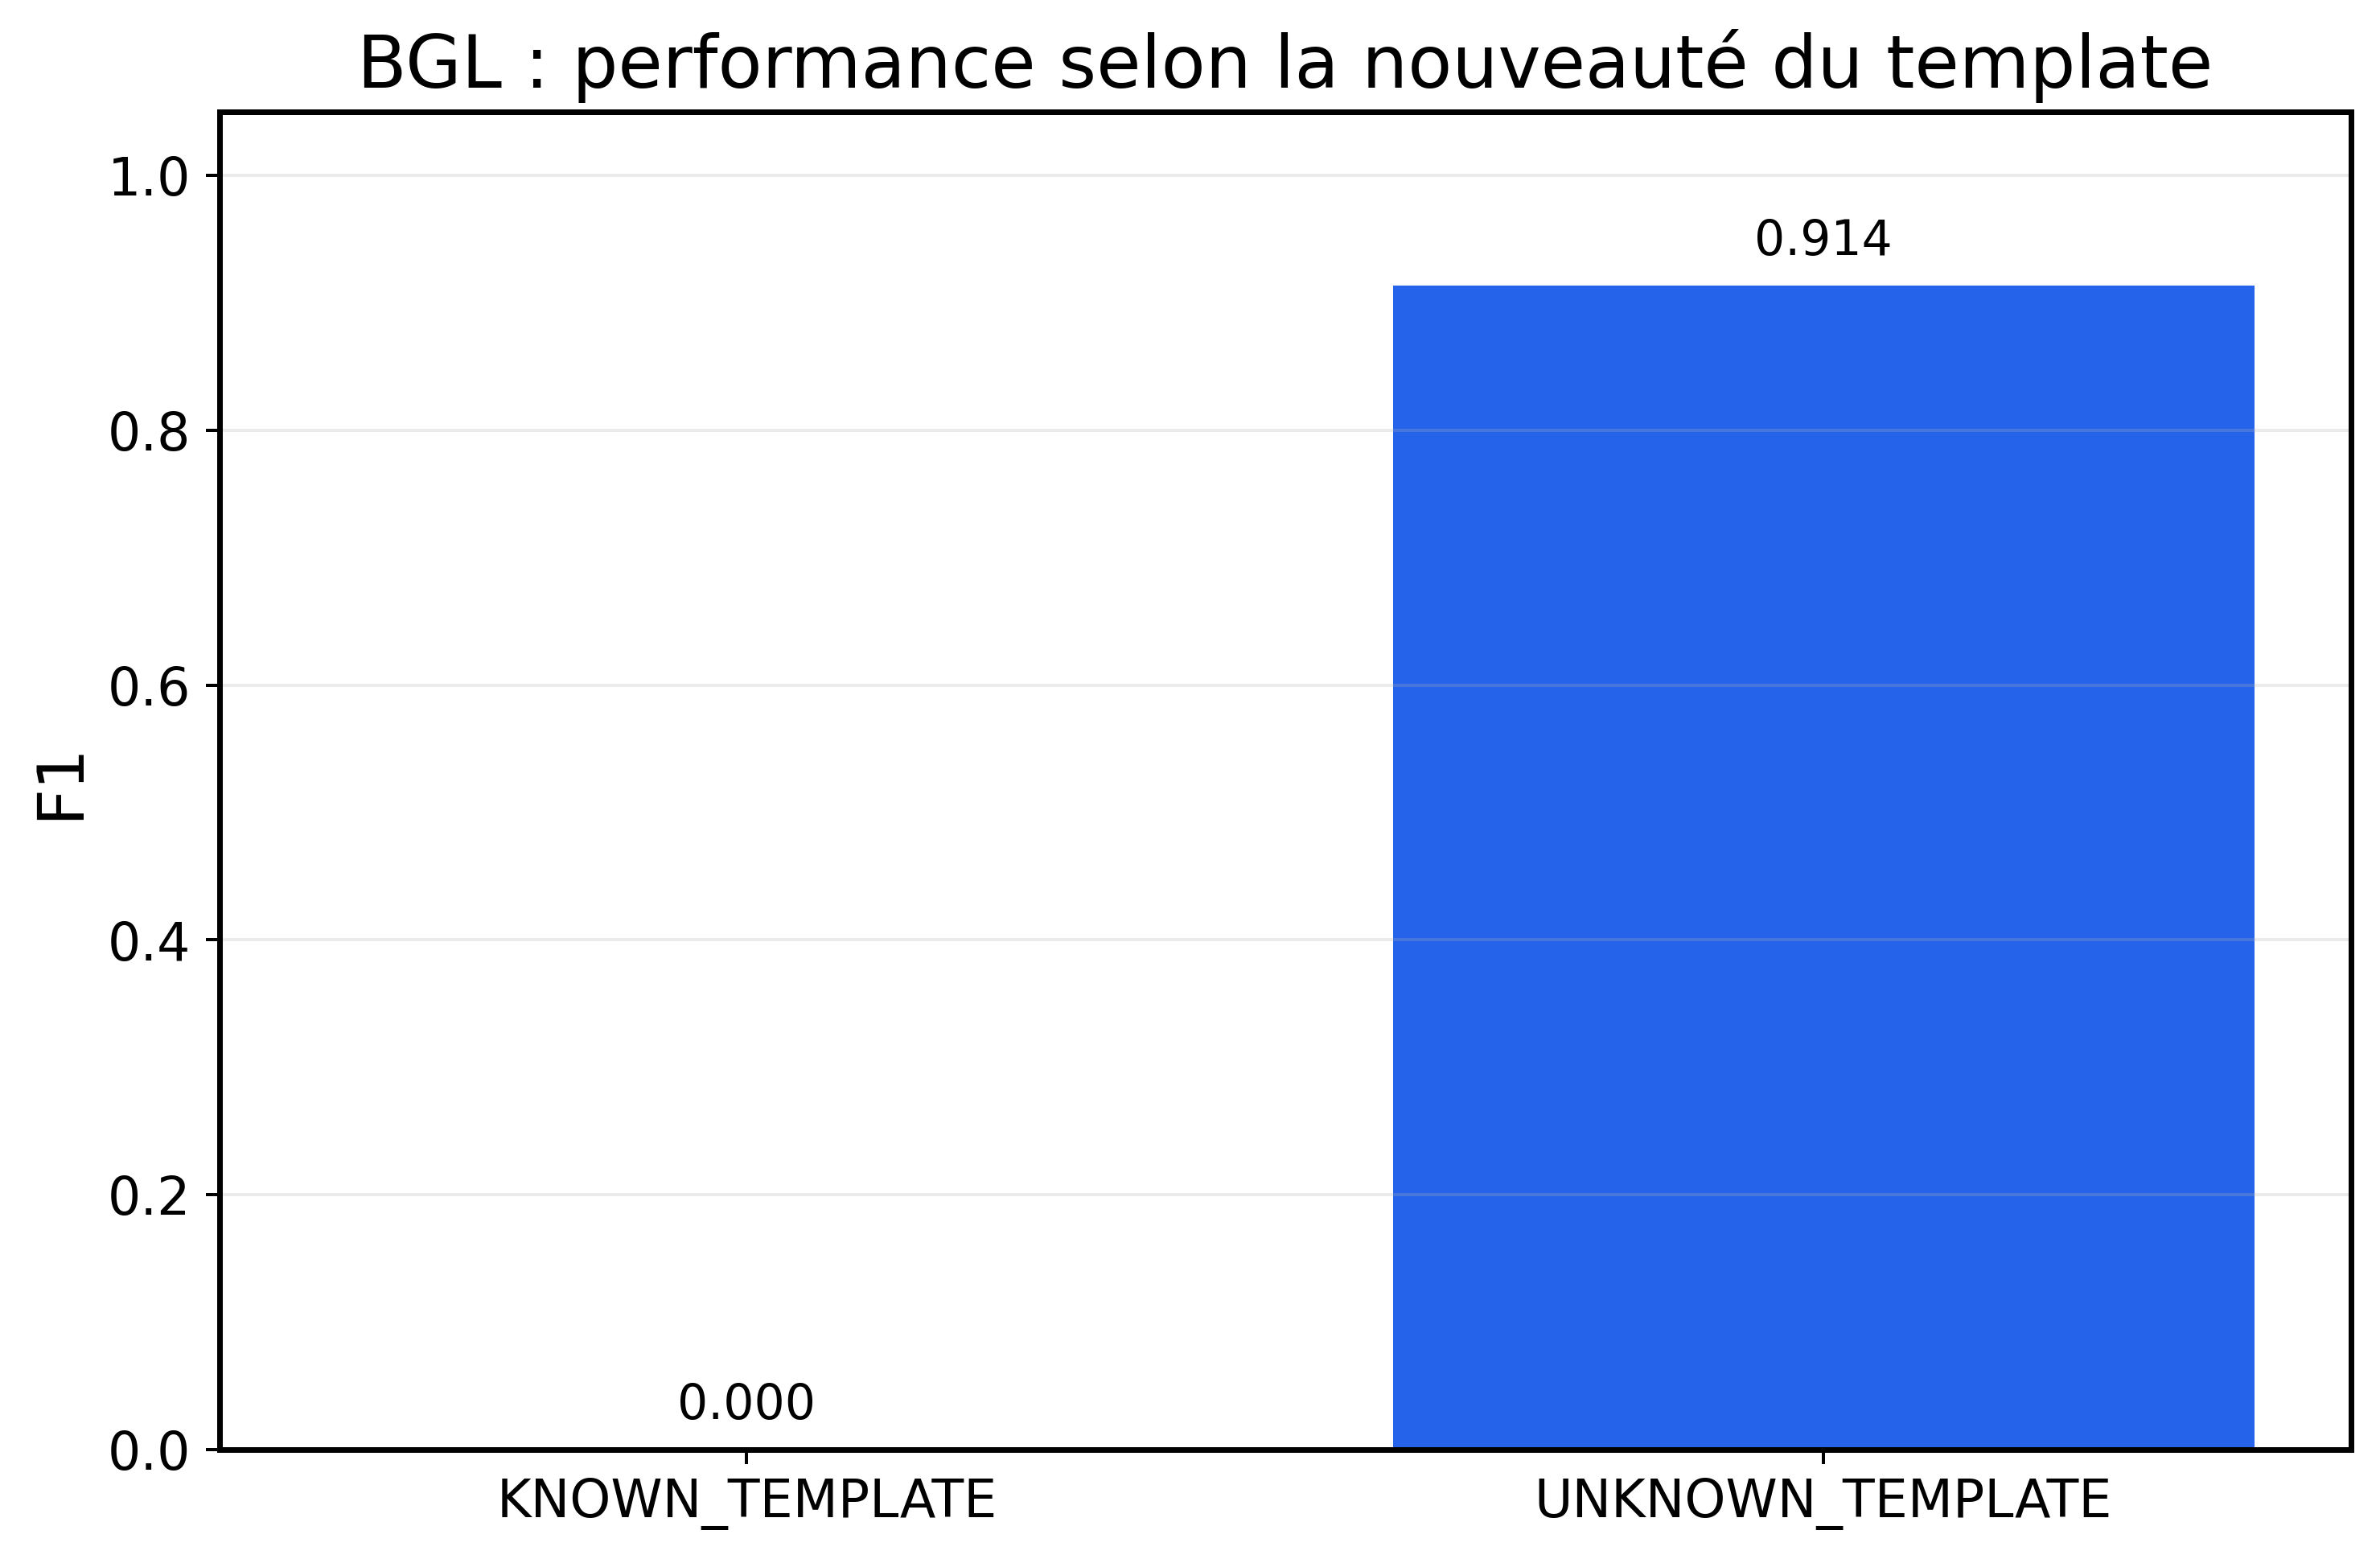
\includegraphics[width=0.78\textwidth]{figures/final/fig_bgl_known_unknown.png}
\caption{BGL : F1 d'Histogram selon que le template est connu ou inconnu au train. Le
groupe connu ne comporte aucune anomalie dans cette partition ; la figure ne permet donc
pas d'estimer un rappel d'anomalies connues.}
\label{fig:bgl-known-unknown-final}
\end{figure}

\begin{figure}[H]
\centering
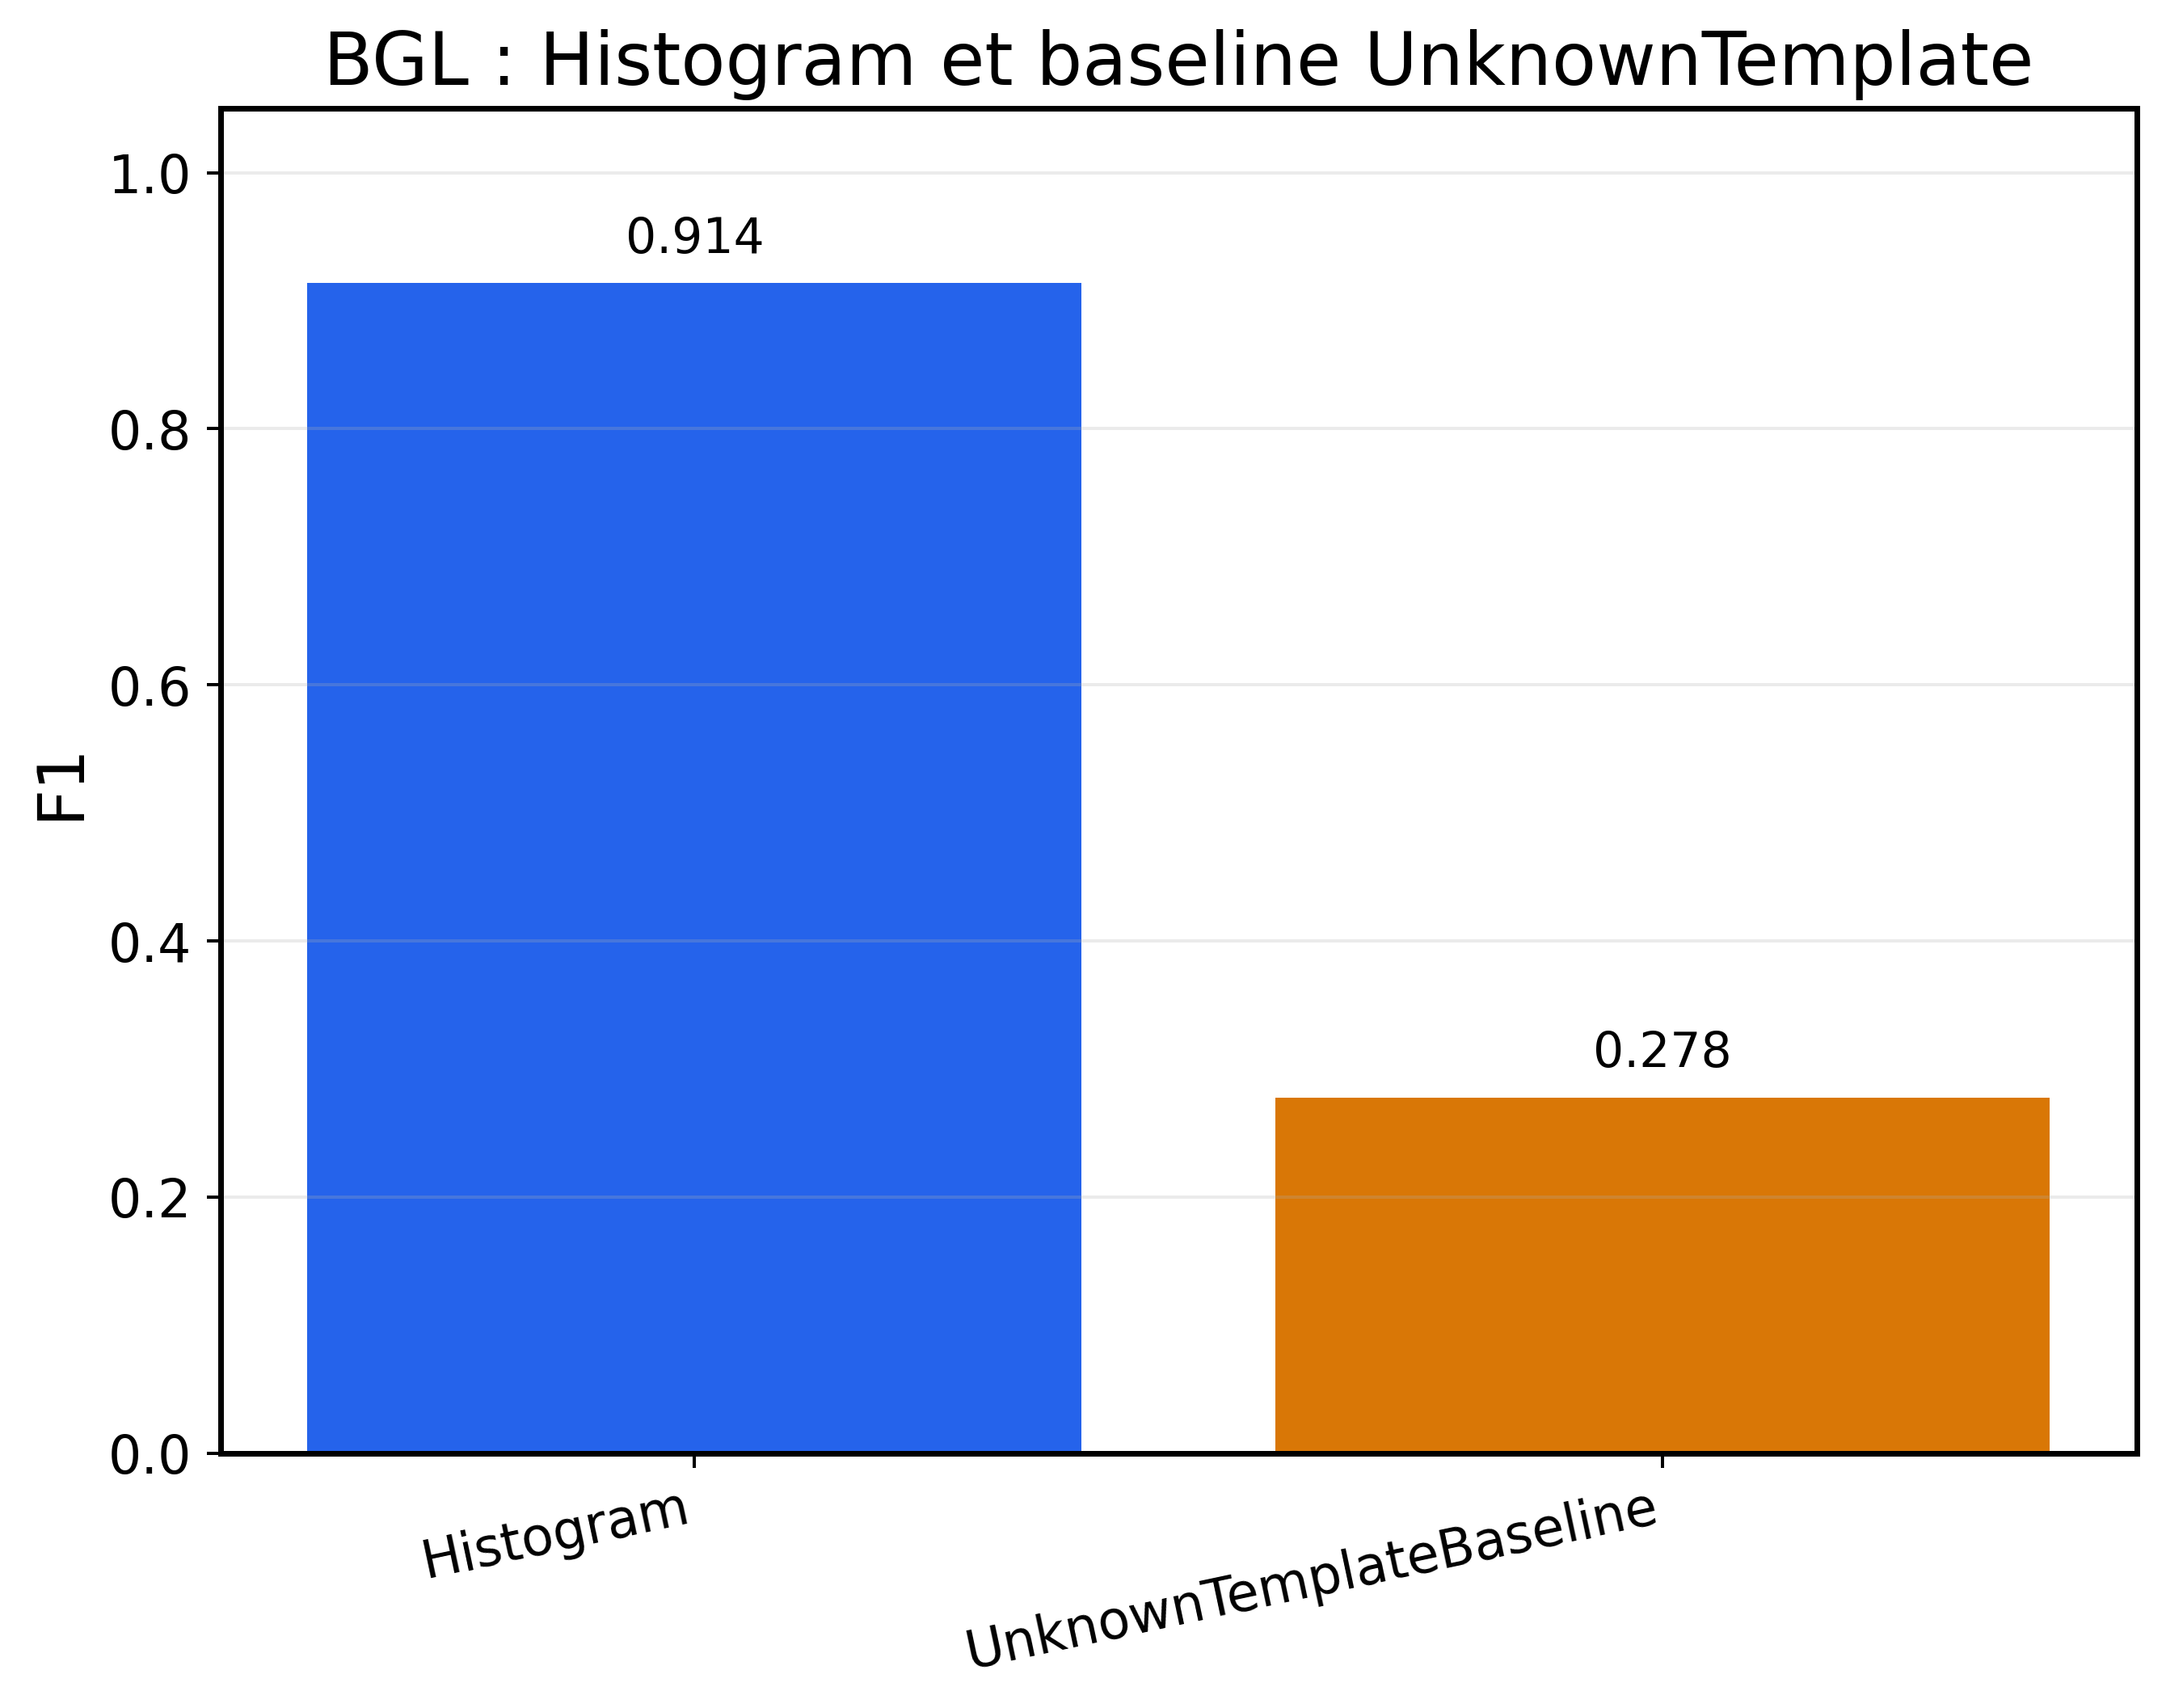
\includegraphics[width=0.78\textwidth]{figures/final/fig_bgl_histogram_vs_unknown_baseline.png}
\caption{BGL : Histogram comparé au baseline qui déclare toute observation inconnue comme
anomalie. L'écart montre que la nouveauté seule n'explique pas tout le score observé.}
\label{fig:bgl-baseline-final}
\end{figure}

\section{Comparaison HDFS/BGL}

Le tableau~\ref{tab:hdfs-bgl-strict} résume les meilleurs résultats stricts retenus.

\begin{table}[H]
\centering
\caption{Résultats du protocole strict HDFS/BGL avec Histogram}
\label{tab:hdfs-bgl-strict}
\small
\begin{tabularx}{\textwidth}{p{2.3cm}p{2.5cm}p{2.3cm}X}
\toprule
\textbf{Dataset} &
\textbf{Méthode} &
\textbf{F1} &
\textbf{Limite importante} \\
\midrule

HDFS &
Histogram, agrégation par \texttt{block\_id} &
$0{,}892308$ &
2\,000 blocs test, 29 positifs ; intervalle bootstrap descriptif et aucune indépendance
statistique revendiquée. \\

BGL &
Histogram &
$0{,}913698$ &
Train sans anomalies et forte proportion de templates test inconnus. \\

\bottomrule
\end{tabularx}
\end{table}

Histogram est déterministe dans cette campagne. Ces deux valeurs correspondent donc à :

\[
N=1.
\]

Il n'existe pas d'écart-type scientifique à leur associer.

La différence entre HDFS et BGL montre également qu'une méthode identique peut se comporter
très différemment selon la structure du journal et le déplacement de distribution.

\section{Mise à jour contrôlée des modèles}

\subsection{Objectif}

La quatrième campagne cherche à vérifier le fonctionnement réel du mécanisme de gouvernance
des modèles.

Trois comportements doivent être observables :

\begin{enumerate}
    \item promotion d'un candidat suffisamment meilleur ;
    \item rejet d'un candidat moins bon ;
    \item rejet d'un candidat légèrement meilleur mais dont le gain reste inférieur au
    seuil minimal.
\end{enumerate}

\subsection{Données}

La campagne utilise le scénario DDoS.

Le train contient :

\[
16\,000 \text{ lignes},
\]

et l'évaluation gelée :

\[
8\,000 \text{ lignes}.
\]

Les données comportent 78 caractéristiques et une prévalence de 0,5.

Trois copies isolées de modèles sont utilisées afin de ne pas modifier les artefacts
principaux sous \texttt{models/} pendant l'expérience.

\subsection{Cas de promotion}

Le modèle courant est Extra Trees et le candidat Random Forest.

Le gain observé est :

\[
\Delta M=+0{,}067845.
\]

Le candidat satisfait la règle de promotion.

L'expérience vérifie également les hashes du modèle courant, du candidat, du backup et du
modèle final.

\subsection{Cas de rejet}

Le modèle courant est Random Forest et le candidat SGDLogistic.

La différence est :

\[
\Delta M=-0{,}063163.
\]

Le candidat étant moins performant selon la métrique retenue, il est rejeté.

Le modèle courant reste actif.

\subsection{Cas d'amélioration insuffisante}

Le troisième cas compare Extra Trees au candidat Logistic Regression.

Le gain est positif :

\[
\Delta M=+0{,}009016.
\]

Cependant, la politique impose :

\[
\delta_{\min}=0{,}02.
\]

Puisque :

\[
0{,}009016 < 0{,}02,
\]

le candidat est rejeté.

Ce résultat est important : le système ne promeut pas un modèle uniquement parce que son
score est légèrement supérieur.

La règle de gouvernance impose une amélioration minimale.

\subsection{Synthèse}

\begin{table}[H]
\centering
\caption{Résultats de la mise à jour contrôlée de bout en bout}
\label{tab:model-update}
\small
\begin{tabularx}{\textwidth}{p{2.6cm}p{3.3cm}p{2.4cm}X}
\toprule
\textbf{Cas} &
\textbf{Comparaison} &
\textbf{$\Delta M$} &
\textbf{Décision} \\
\midrule

Promotion &
Extra Trees $\rightarrow$ Random Forest &
$+0{,}067845$ &
Candidat promu. \\

Dégradation &
Random Forest $\rightarrow$ SGDLogistic &
$-0{,}063163$ &
Candidat rejeté. \\

Gain insuffisant &
Extra Trees $\rightarrow$ Logistic Regression &
$+0{,}009016$ &
Rejet car gain inférieur à $\delta_{\min}=0{,}02$. \\

\bottomrule
\end{tabularx}
\end{table}

La campagne démontre donc fonctionnellement la procédure de mise à jour contrôlée.

Elle ne constitue pas une preuve d'apprentissage continu autonome en production.

\IfFileExists{figures/model_update_promotion_rejet.png}{
\begin{figure}[H]
\centering

\includegraphics[width=0.82\textwidth]{figures/model_update_promotion_rejet.png}
\caption{Comportement de la procédure de promotion et de rejet des modèles candidats.}
\label{fig:model-update}
\end{figure}

\begin{center}
\footnotesize Source : auteur, à partir des résultats expérimentaux de ce travail.
\end{center}
}{}

\section{Validation multiformat}

\subsection{Objectif}

L'architecture prévoit plusieurs adaptateurs. L'objectif de cette expérience est de
vérifier quelles voies produisent réellement une sortie normalisée avec l'implémentation
finale.

Huit voies sont testées :

\begin{enumerate}
    \item Windows EVTX ;
    \item Linux/auth tabulaire ;
    \item Wazuh CSV ;
    \item syslog ;
    \item Apache ;
    \item HDFS ;
    \item BGL ;
    \item réseau tabulaire.
\end{enumerate}

Un maximum de 1\,000 unités est prélevé en ordre source pour chaque voie lorsque la source
le permet.

Aucune duplication artificielle n'est utilisée pour augmenter le nombre de cas.

Apache constitue un cas particulier avec une fixture synthétique de taille :

\[
N=1.
\]

\subsection{Mesures}

La campagne enregistre notamment :

\begin{itemize}
    \item unités brutes ;
    \item unités lues ;
    \item unités parsées ;
    \item unités normalisées ;
    \item erreurs ;
    \item pertes ;
    \item complétude des champs communs ;
    \item conservation exacte du message lorsqu'elle peut être testée.
\end{itemize}

Le routage n'est pas évalué dans cette même expérience afin de ne pas mélanger les deux
fonctions.

\subsection{Résultat global}

Au total, les compteurs finaux donnent :

\[
\text{lues}=7\,001,\qquad
\text{parsées}=7\,001,\qquad
\text{normalisées}=7\,001.
\]

La couverture de la chaîne d'adaptateurs est donc de $7\,001/7\,001$ pour cette
campagne. Cette couverture ne signifie ni que tous les champs sont renseignés ni que le
message brut est conservé intégralement pour chaque format.

\subsection{HDFS et BGL}

Les contrôles par voie donnent également :

\[
\mathrm{HDFS}: 1\,000/1\,000,
\]

\[
\mathrm{BGL}: 1\,000/1\,000.
\]

Ces résultats concernent la campagne multiformat finale et ne doivent pas être mélangés
avec les sorties historiques de la voie exploratoire. Le pipeline strict HDFS/BGL et la
voie multiformat utilisent des adaptateurs et des représentations distincts ; la
couverture de lecture/parsing/normalisation ne remplace donc pas l'évaluation prédictive
au niveau bloc ou au niveau template.

\subsection{Conservation exacte du message}

La campagne mesure également la conservation exacte du message lorsque cette vérification
est possible.

Cette propriété n'est pas universellement satisfaite.

Il n'est donc pas correct de présenter le prototype comme garantissant la conservation
bit-à-bit du brut pour toutes les sources.

L'objectif architectural de traçabilité reste pertinent, mais sa couverture effective
dépend des adaptateurs.

\subsection{Conclusion}

La formulation scientifiquement soutenue est :

\begin{quote}
\textit{La validation multiformat est fonctionnelle mais partielle.}
\end{quote}

Elle démontre que plusieurs voies sont effectivement utilisables et identifie simultanément
deux échecs importants.

\IfFileExists{figures/validation_multiformat.png}{
\begin{figure}[H]
\centering

\includegraphics[width=0.88\textwidth]{figures/validation_multiformat.png}
\caption{Résultats de la validation multiformat du pipeline.}
\label{fig:multiformat}
\end{figure}

\begin{center}
\footnotesize Source : auteur, à partir des résultats expérimentaux de ce travail.
\end{center}
}{}

\begin{figure}[H]
\centering
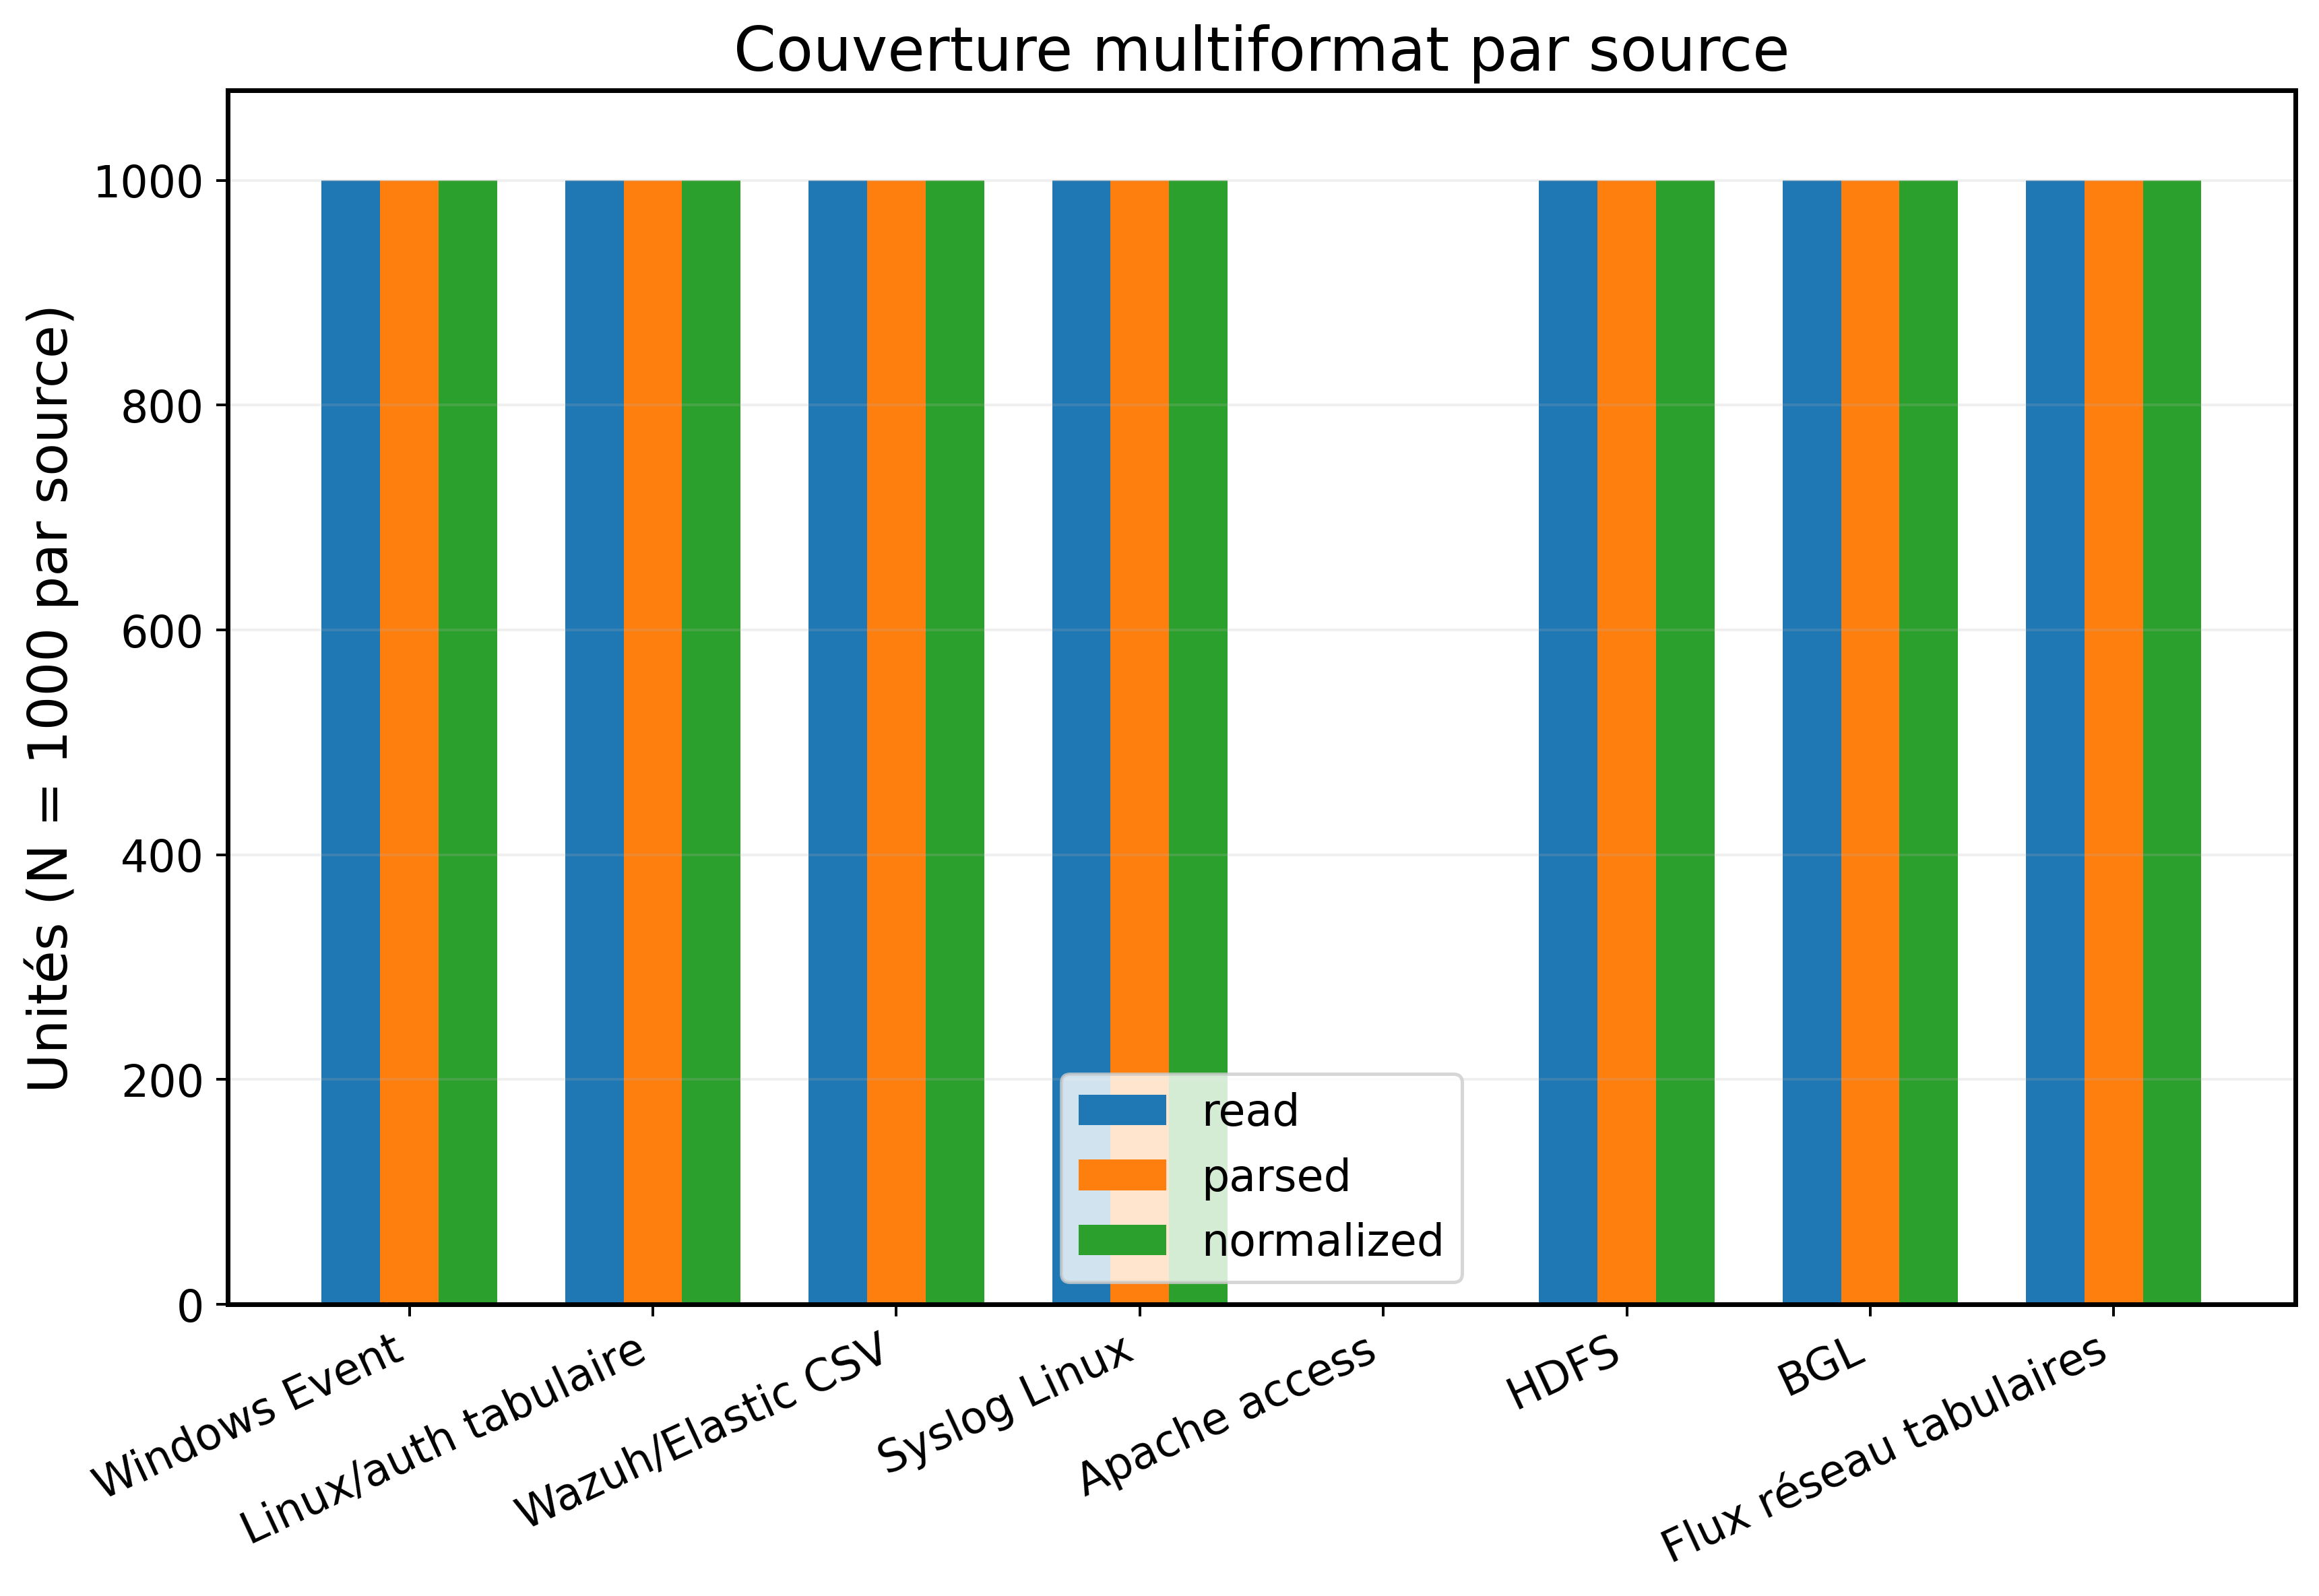
\includegraphics[width=0.96\textwidth]{figures/final/fig_multiformat_coverage_by_source.png}
\caption{Couverture multiformat par source dans la campagne finale. Les compteurs de
lecture, parsing et normalisation sont extraits du CSV ; Apache reste une fixture d'une
seule ligne et la complétude des champs n'est pas assimilée à une équivalence sémantique.}
\label{fig:multiformat-coverage-final}
\end{figure}

\section{Évaluation du routeur réel}

\subsection{Protocole}

Le routeur est évalué séparément du parser afin d'isoler sa fonction.

Neuf sources hashées sont utilisées.

Elles sont divisées en chunks de 100 lignes lorsque leur taille le permet.

Les noms attribués aux chunks sont neutralisés pour limiter l'utilisation directe du nom
de la source comme réponse.

Apache reste un cas particulier avec :

\[
N=1.
\]

Le corpus final comporte :

\[
81 \text{ fichiers}.
\]

La vérité de famille est fixée avant l'exécution du routeur.

Pour chaque fichier, la campagne enregistre :

\begin{itemize}
    \item famille réelle ;
    \item famille prédite ;
    \item modèle choisi ;
    \item scores ;
    \item raisons ;
    \item marge ;
    \item fallback ;
    \item erreur ;
    \item existence de l'artefact de modèle.
\end{itemize}

\subsection{Résultat}

Le routeur attribue correctement :

\[
80/81
\]

fichiers.

L'exactitude est :

\[
0{,}987654.
\]

Le F1 macro calculé sur l'union des familles vaut :

\[
0{,}883598.
\]

L'unique erreur principale concerne le cas Apache, orienté vers le fallback.

\subsection{Interprétation}

La performance est élevée dans ce corpus.

Elle doit néanmoins être limitée au corpus dérivé utilisé.

Les chunks issus d'une même source ne sont pas statistiquement indépendants. Ils peuvent
partager la même structure et des caractéristiques très similaires.

De plus, certaines métadonnées du fichier peuvent révéler indirectement la famille.

Le résultat constitue donc une validation fonctionnelle forte du routeur sur le corpus
local retenu, mais pas une estimation de sa performance sur toute source inconnue.

\subsection{Confidence}

La confidence enregistrée est une marge entre les deux meilleurs scores heuristiques.

Elle ne constitue pas une probabilité.

Aucune calibration probabiliste n'est réalisée dans ce protocole.

\subsection{Contrôle open-set consolidé}

Une seconde évaluation sépare l'attribution connue du rejet de sources inconnues. La
politique est calibrée par validation leave-one-family-out en retirant à tour de rôle une
famille connue ; les trois fichiers open-set finaux ne participent pas au réglage du
seuil. La politique retenue est $\texttt{top\_score}\geq100$.

Sur le test final gelé, les 28 fichiers connus sont tous acceptés correctement et les
trois fichiers inconnus sont rejetés :

\[
\text{faux rejet connu}=0/28,\qquad
\text{rejet inconnu}=3/3,\qquad
\text{coverage}=0{,}903226.
\]

La marge \texttt{decision\_margin} demeure un score heuristique de séparation et non une
probabilité calibrée. Ce résultat soutient le fonctionnement de la politique sur le
corpus local testé ; il ne permet pas de conclure à un rejet open-set général.

\IfFileExists{figures/router_confusion_matrix.png}{
\begin{figure}[H]
\centering

\includegraphics[width=0.78\textwidth]{figures/router_confusion_matrix.png}
\caption{Matrice de confusion du routeur sur le corpus dérivé de 81 fichiers.}
\label{fig:router-confusion}
\end{figure}

\begin{center}
\footnotesize Source : auteur, à partir des résultats expérimentaux de ce travail.
\end{center}
}{}

\begin{figure}[H]
\centering
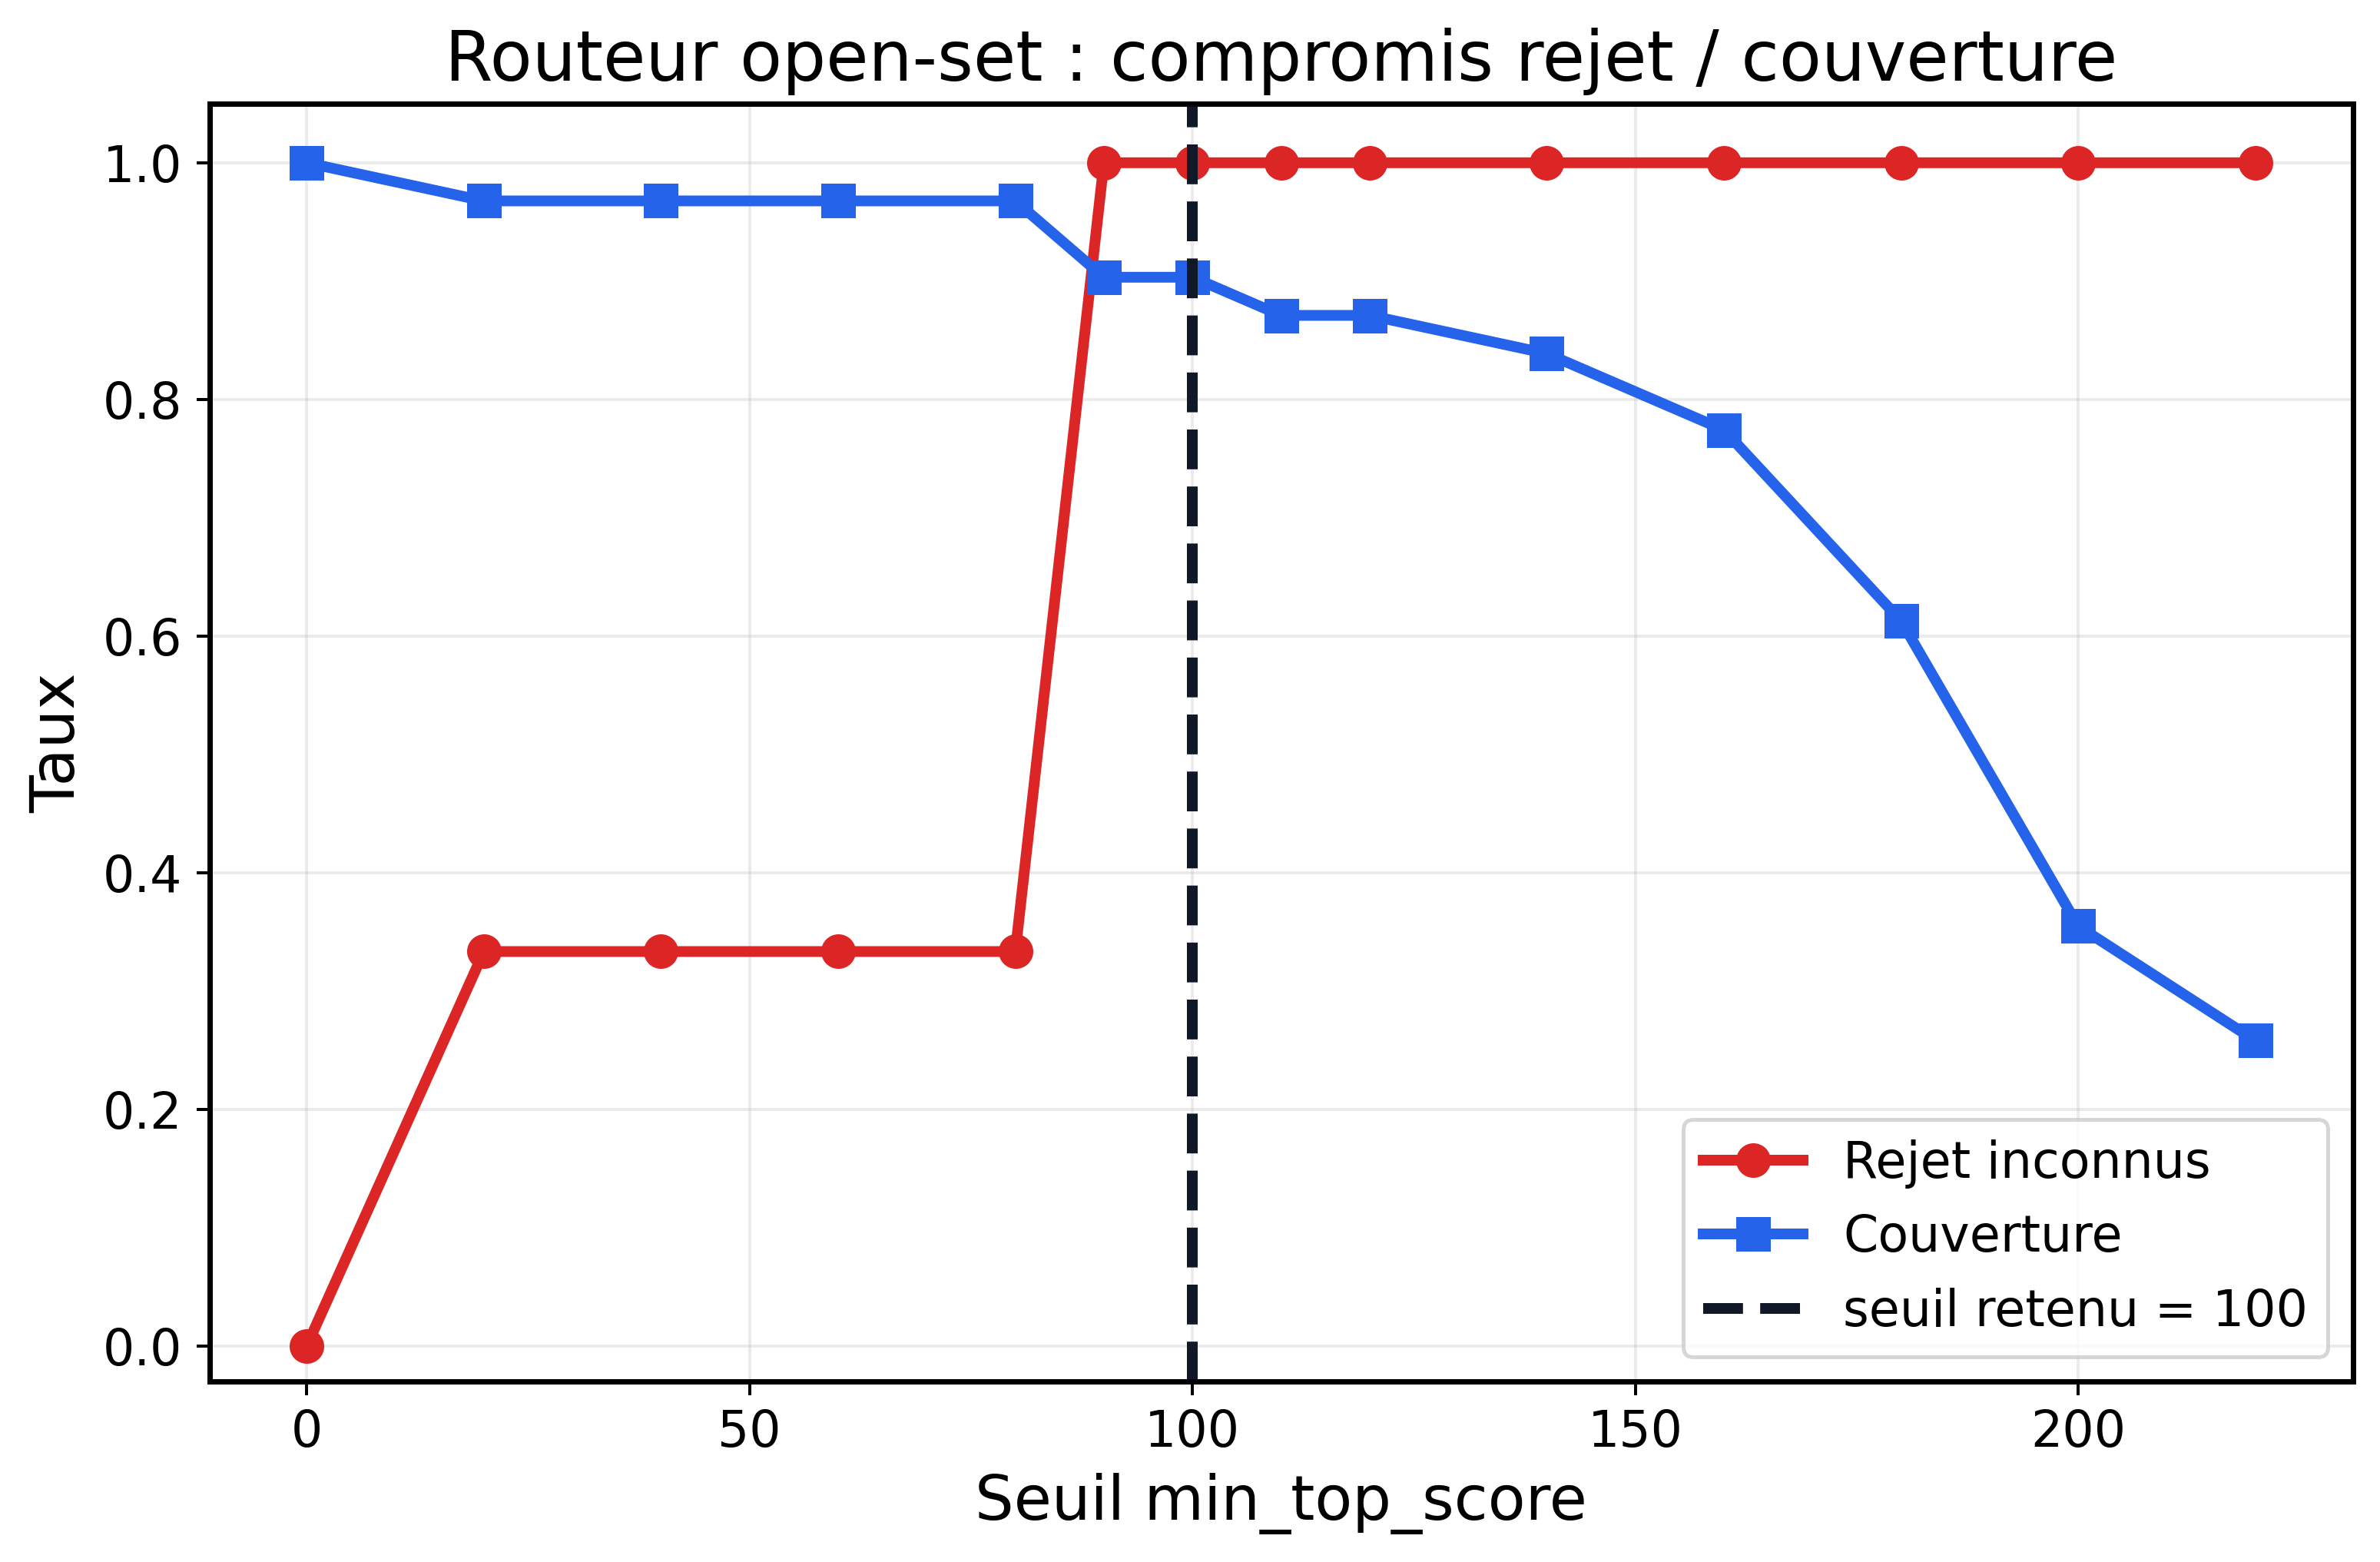
\includegraphics[width=0.88\textwidth]{figures/final/fig_router_open_set_tradeoff.png}
\caption{Diagnostic du compromis open-set du routeur. Le seuil retenu sur la validation
($\texttt{top\_score}\geq100$) rejette les trois fichiers inconnus du test sans faux rejet
parmi les 28 fichiers connus ; la marge reste une heuristique non calibrée.}
\label{fig:router-open-set-tradeoff-final}
\end{figure}

\section{Routage spécialisé et performance prédictive}

La bonne attribution d'une famille et l'amélioration de la prédiction sont deux questions
différentes.

Une ablation complémentaire compare, sur plusieurs configurations, un traitement global à
un traitement spécialisé.

Les résultats vérifiés sur les voies retenues ne montrent pas une amélioration
systématique.

Pour CICIDS :

\[
F_{1,\mathrm{global}}=0{,}999132,
\]

\[
F_{1,\mathrm{spécialisé}}=0{,}999333,
\]

soit :

\[
\Delta F_1=+0{,}000201.
\]

Sur Linux/auth :

\[
F_{1,\mathrm{global}}=0{,}819404,
\]

\[
F_{1,\mathrm{spécialisé}}=0{,}816354,
\]

soit :

\[
\Delta F_1=-0{,}003050.
\]

Une troisième voie de l'ablation possède une traçabilité de dataset insuffisante pour
servir de résultat principal dans ce mémoire et n'est donc pas utilisée pour tirer une
conclusion quantitative supplémentaire.

Les deux résultats détaillés ici suffisent déjà à montrer que la spécialisation n'apporte
pas mécaniquement un gain.

L'intérêt principal du routage est donc architectural :

\begin{itemize}
    \item éviter des incompatibilités de format ;
    \item appliquer le prétraitement correspondant ;
    \item sélectionner un artefact compatible ;
    \item faciliter l'extension du pipeline.
\end{itemize}

\section{Contrôles complémentaires sur CSE-CIC-IDS2018}

Le contrôle externe utilise le split documenté du 15 février 2018 vers le 16 février
2018, 78 caractéristiques et cinq seeds. La régression logistique atteint un F1 moyen de
$0{,}999212$, contre $0{,}401375$ pour Random Forest. Ce résultat est conservé avec les
contrôles mono-caractéristique, d'ablation et de permutation ; il ne permet pas d'affirmer
l'absence de fuite, mais il identifie les mécanismes testés et leurs effets.

\begin{figure}[H]
\centering
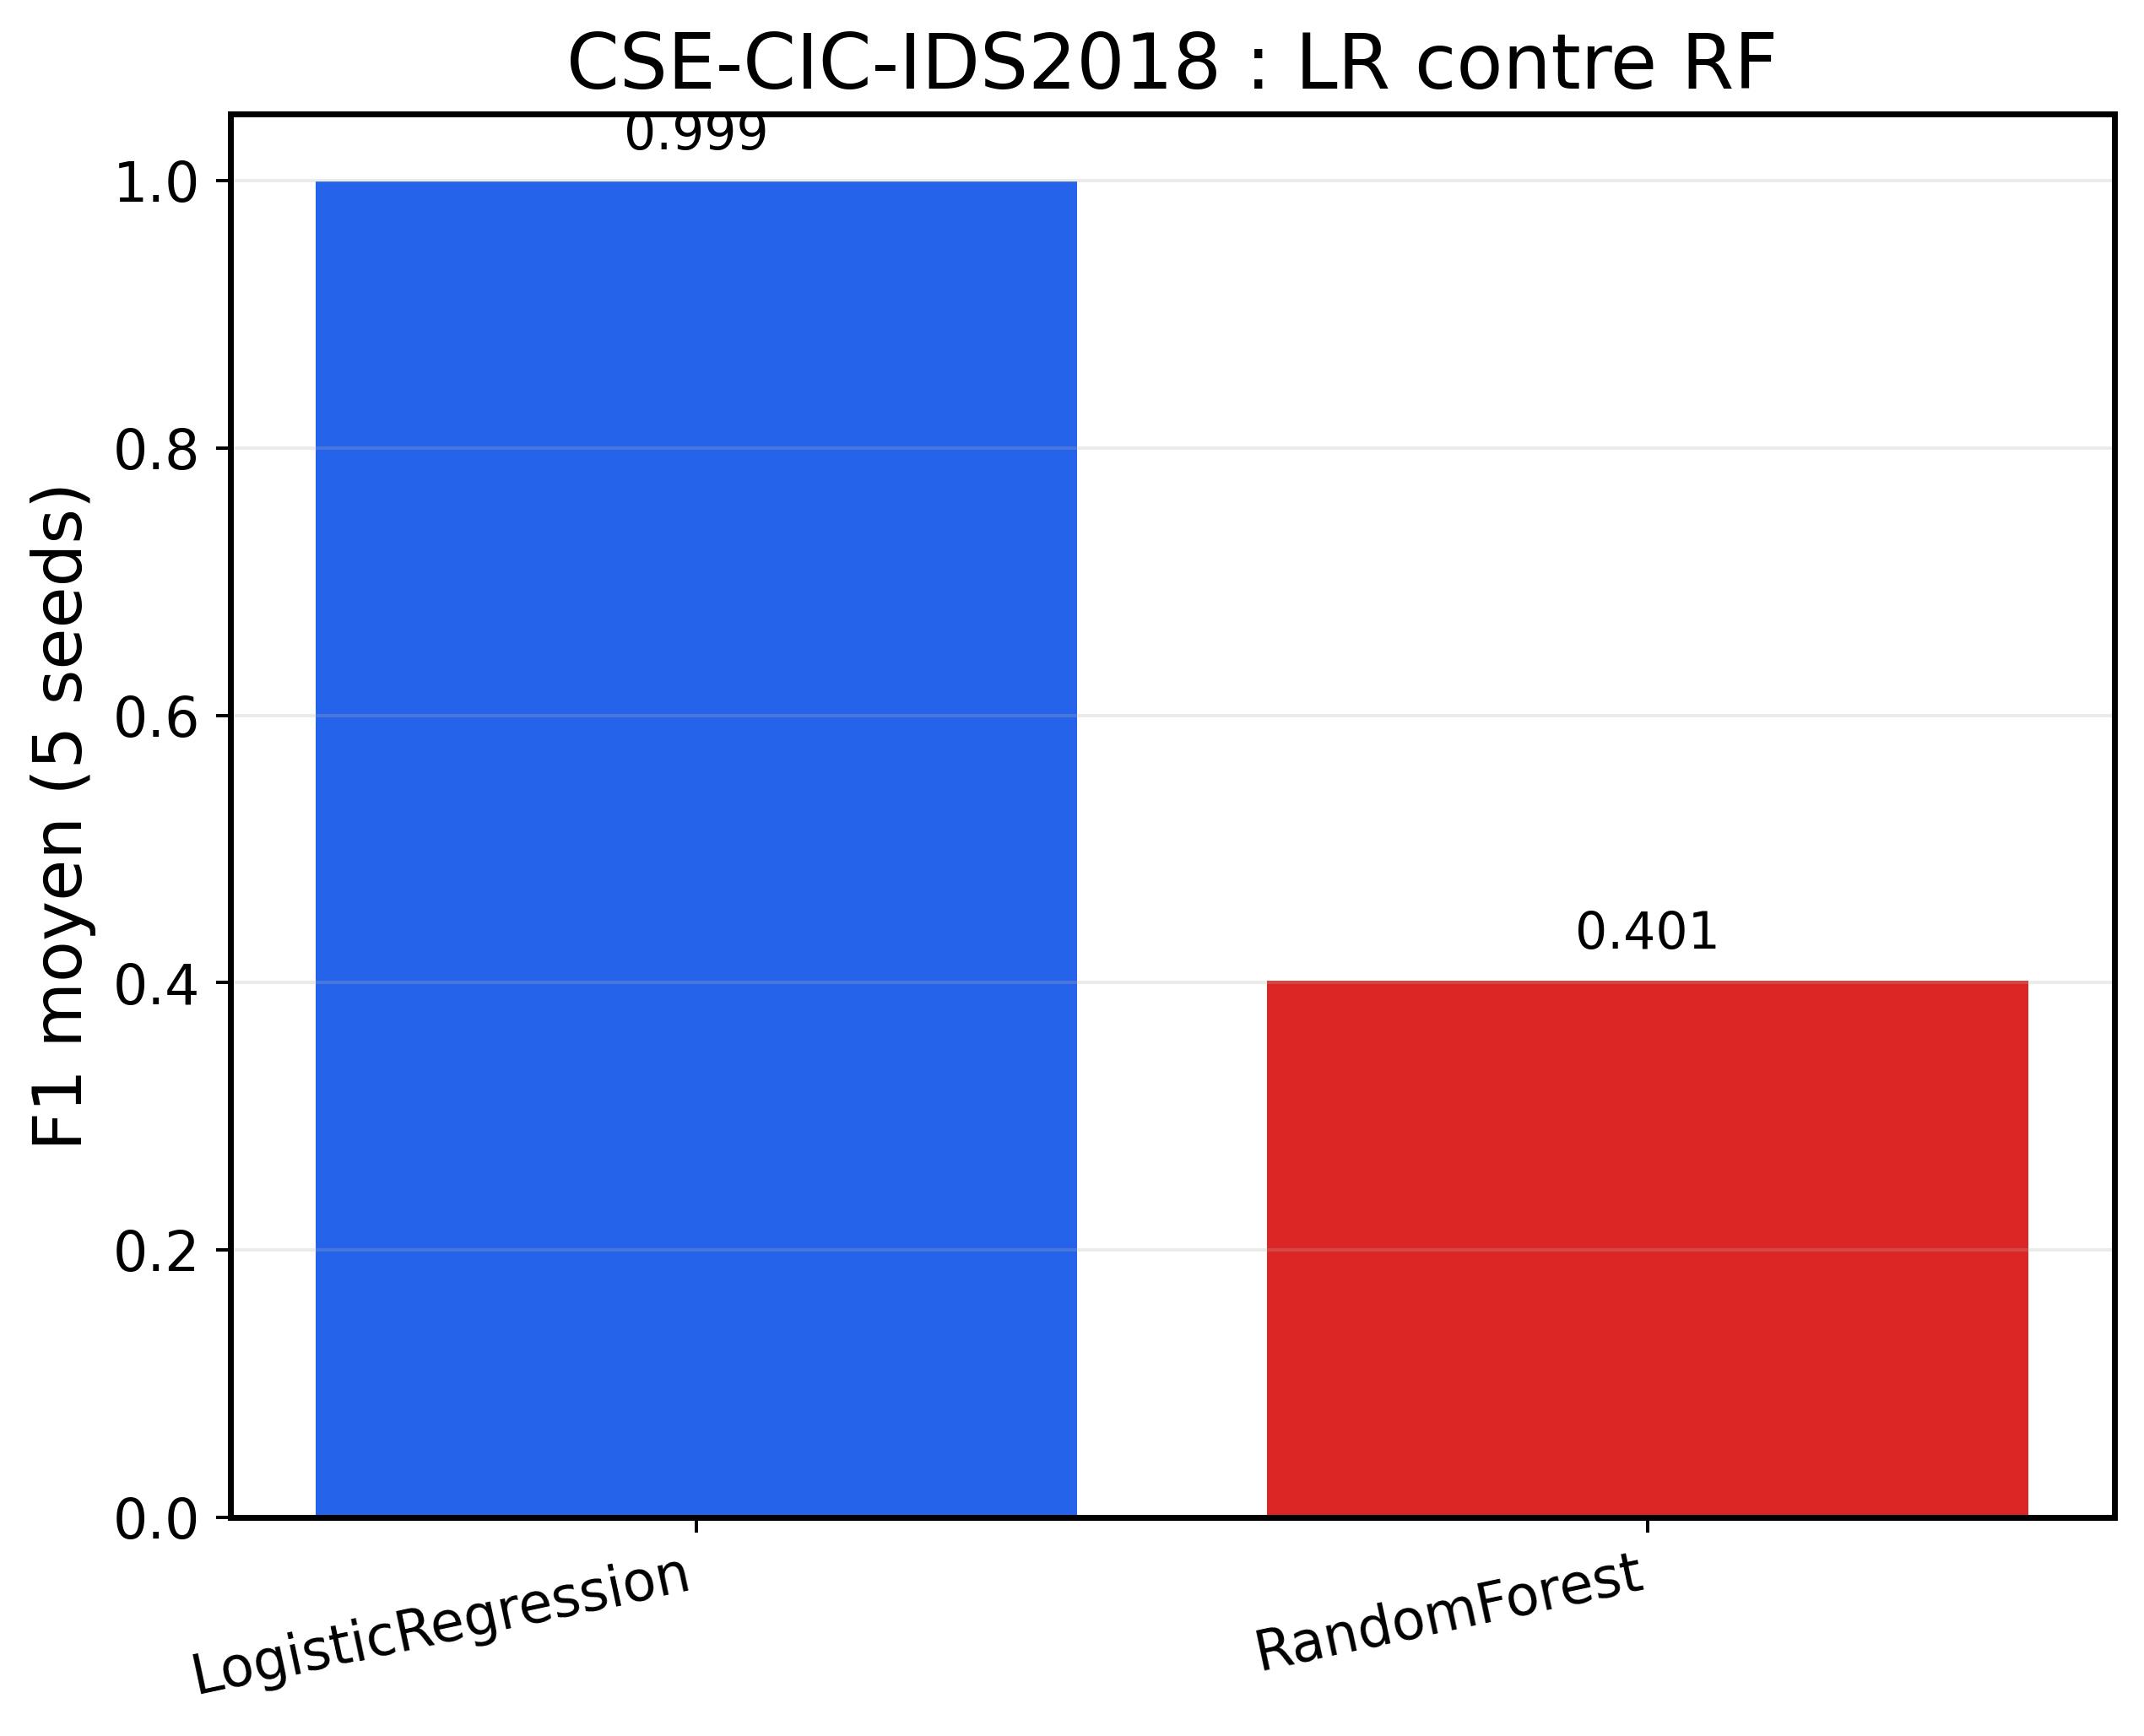
\includegraphics[width=0.76\textwidth]{figures/final/fig_csecic_lr_vs_rf.png}
\caption{CSE-CIC-IDS2018 : comparaison LR/RF sur le split 2018-02-15 vers 2018-02-16
(cinq seeds).}
\label{fig:csecic-lr-rf-final}
\end{figure}

\begin{figure}[H]
\centering
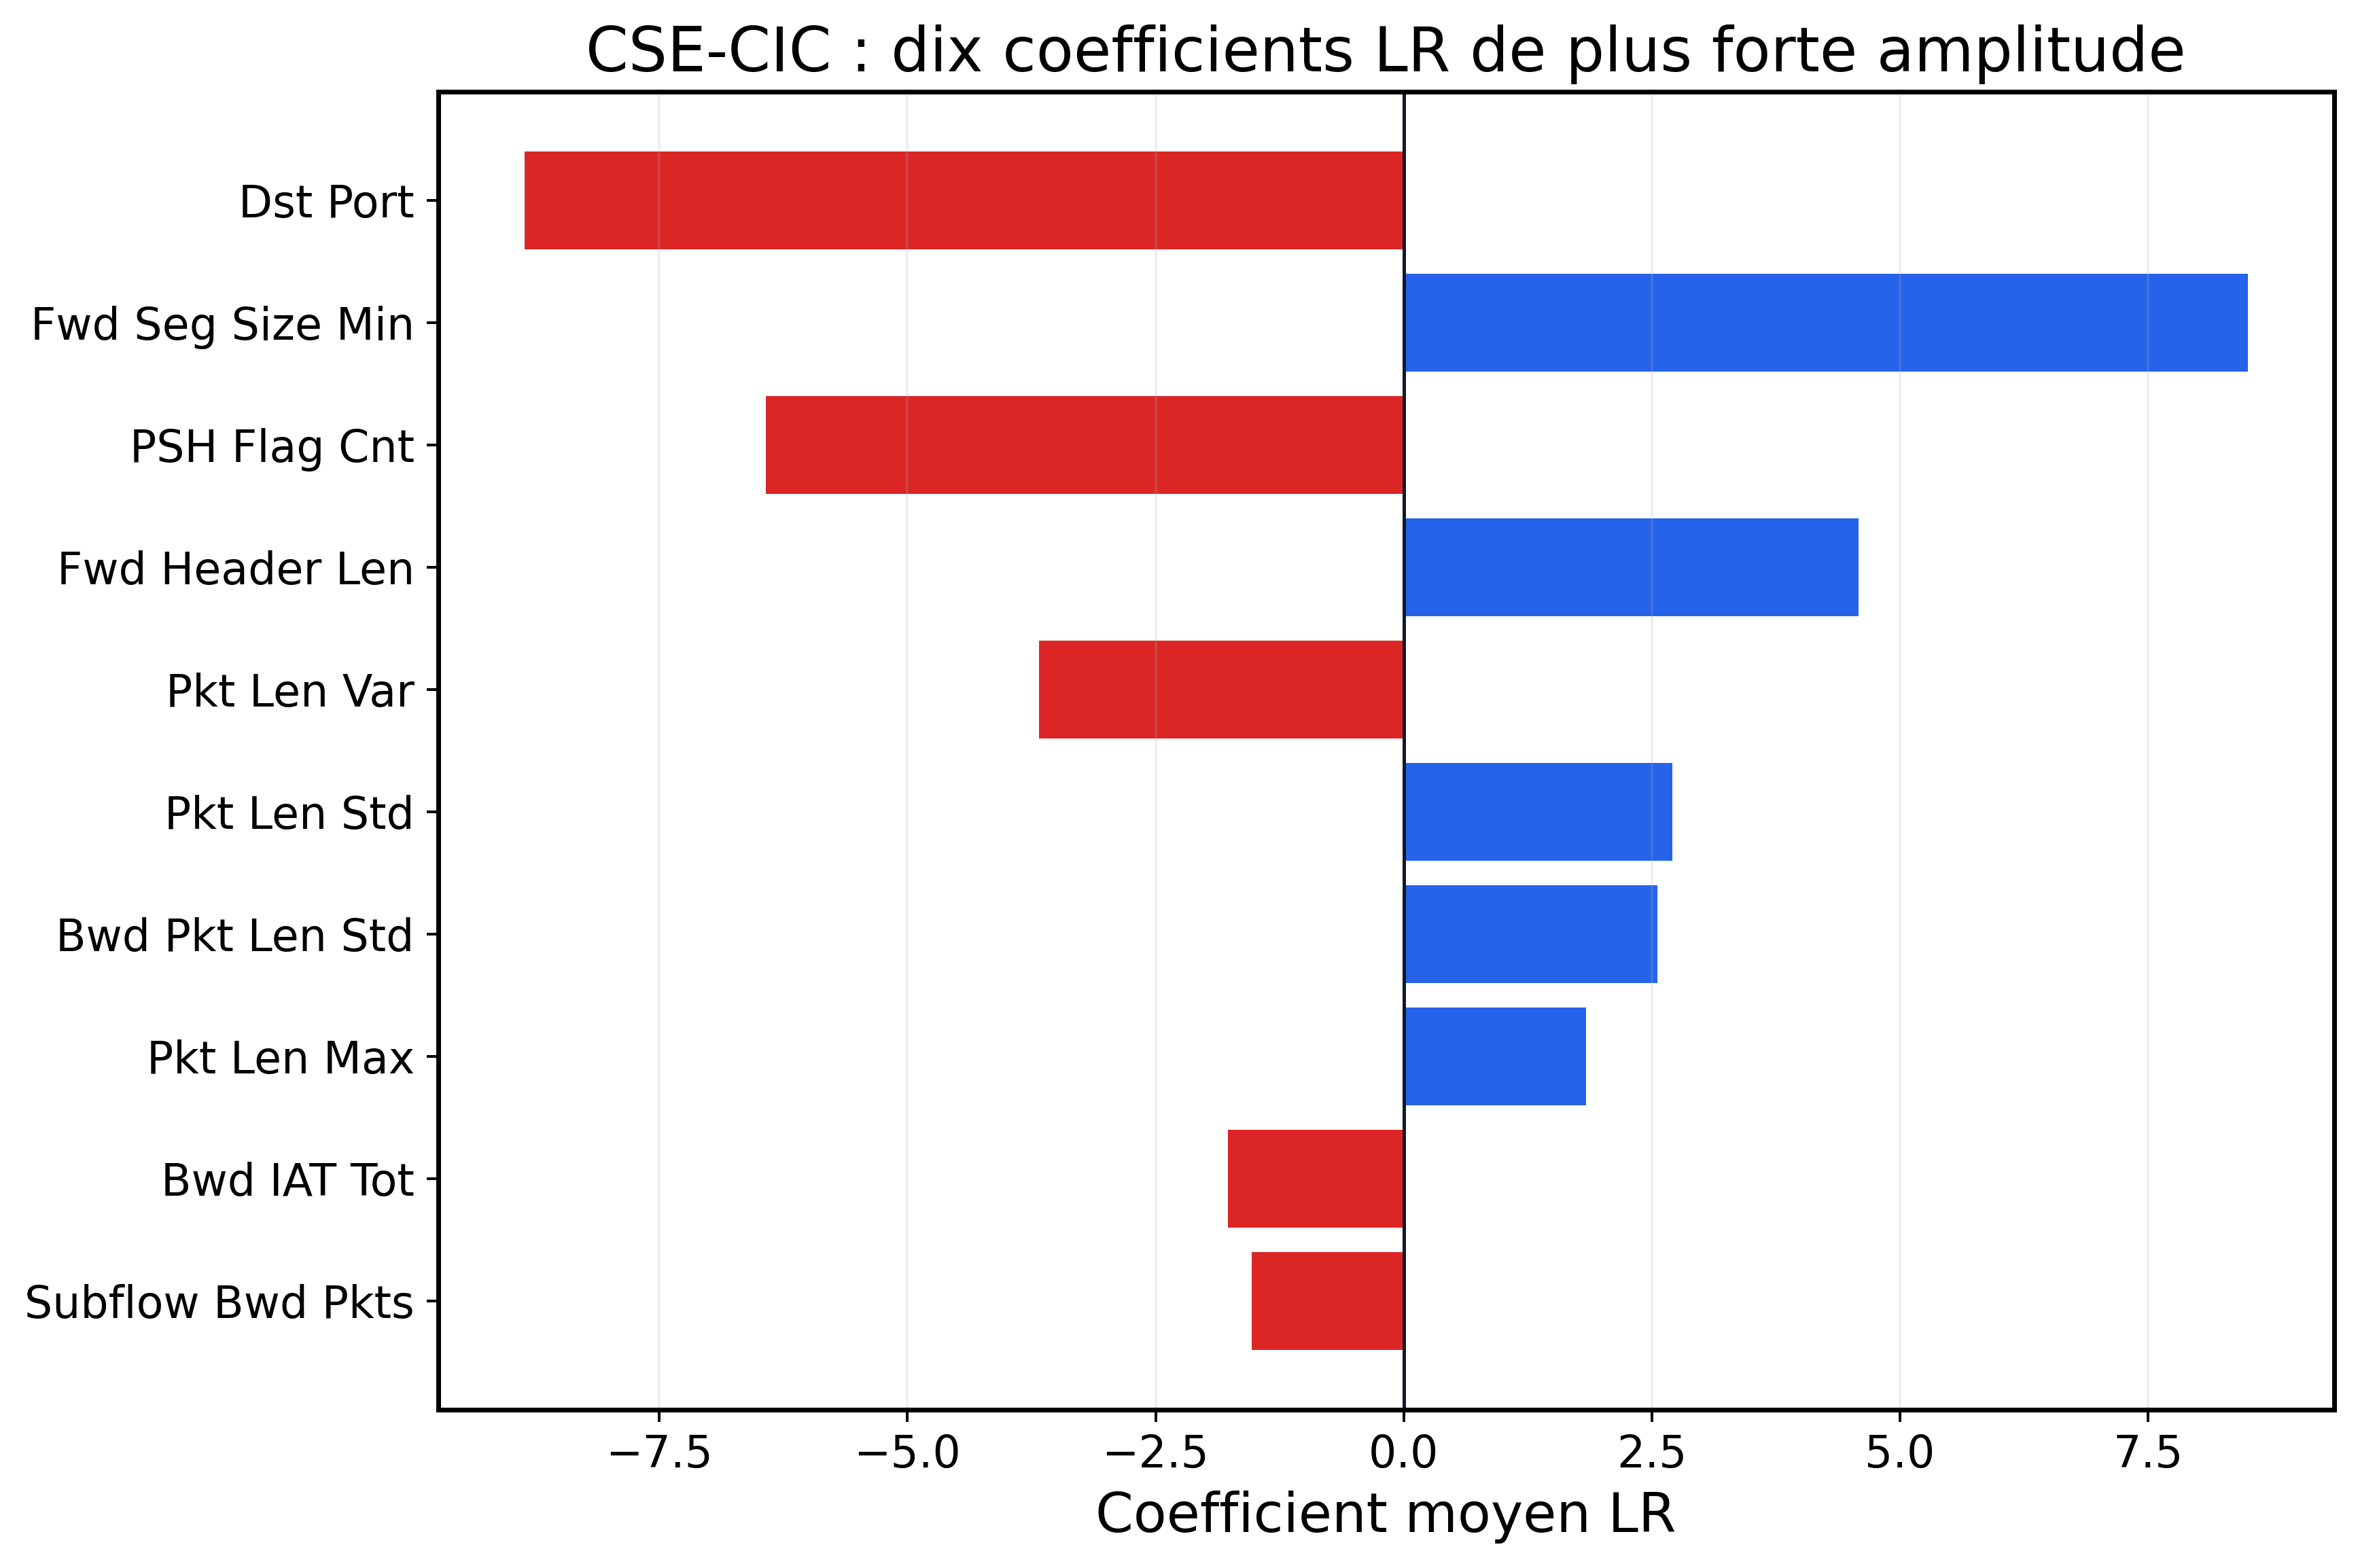
\includegraphics[width=0.95\textwidth]{figures/final/fig_csecic_lr_coefficients.png}
\caption{Dix coefficients de plus forte amplitude de la régression logistique CSE-CIC.
Ils décrivent les associations apprises et ne constituent pas une interprétation causale.}
\label{fig:csecic-coefficients-final}
\end{figure}

\begin{figure}[H]
\centering
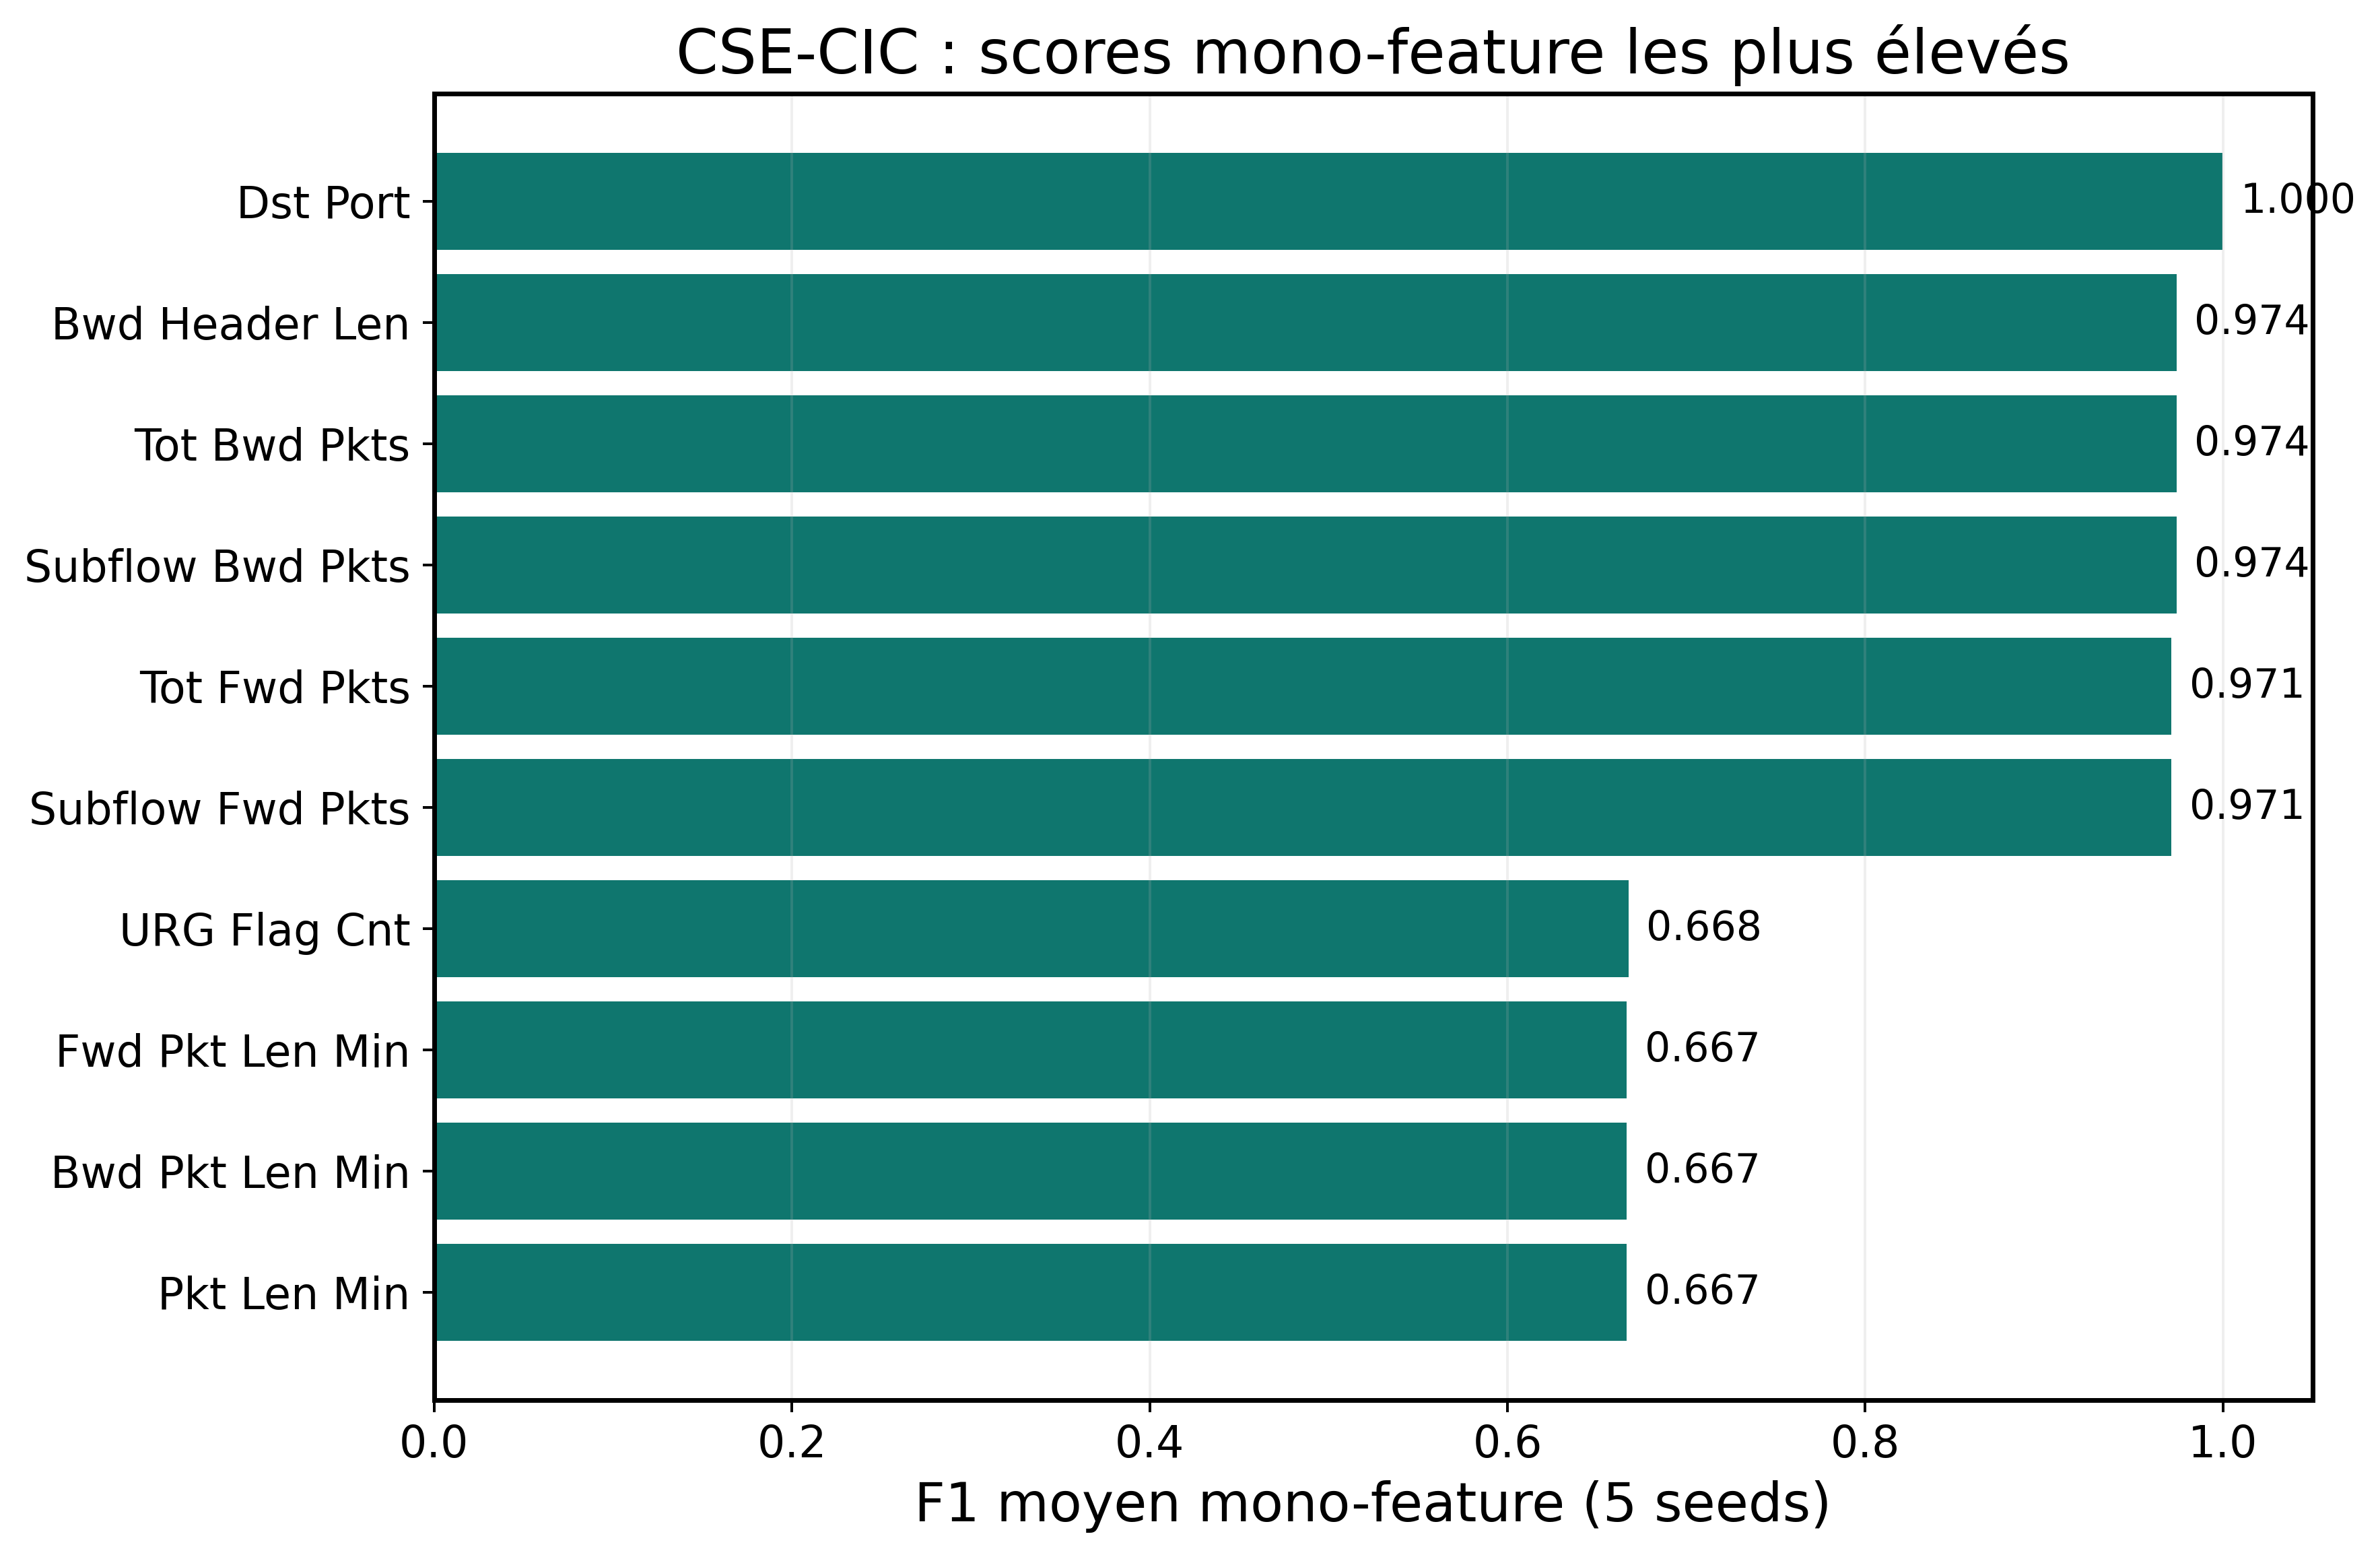
\includegraphics[width=0.92\textwidth]{figures/final/fig_csecic_lr_single_feature.png}
\caption{Scores F1 mono-caractéristique les plus élevés sur CSE-CIC (cinq seeds). La
performance de Dst Port motive les contrôles de robustesse complémentaires.}
\label{fig:csecic-single-feature-final}
\end{figure}

\begin{figure}[H]
\centering
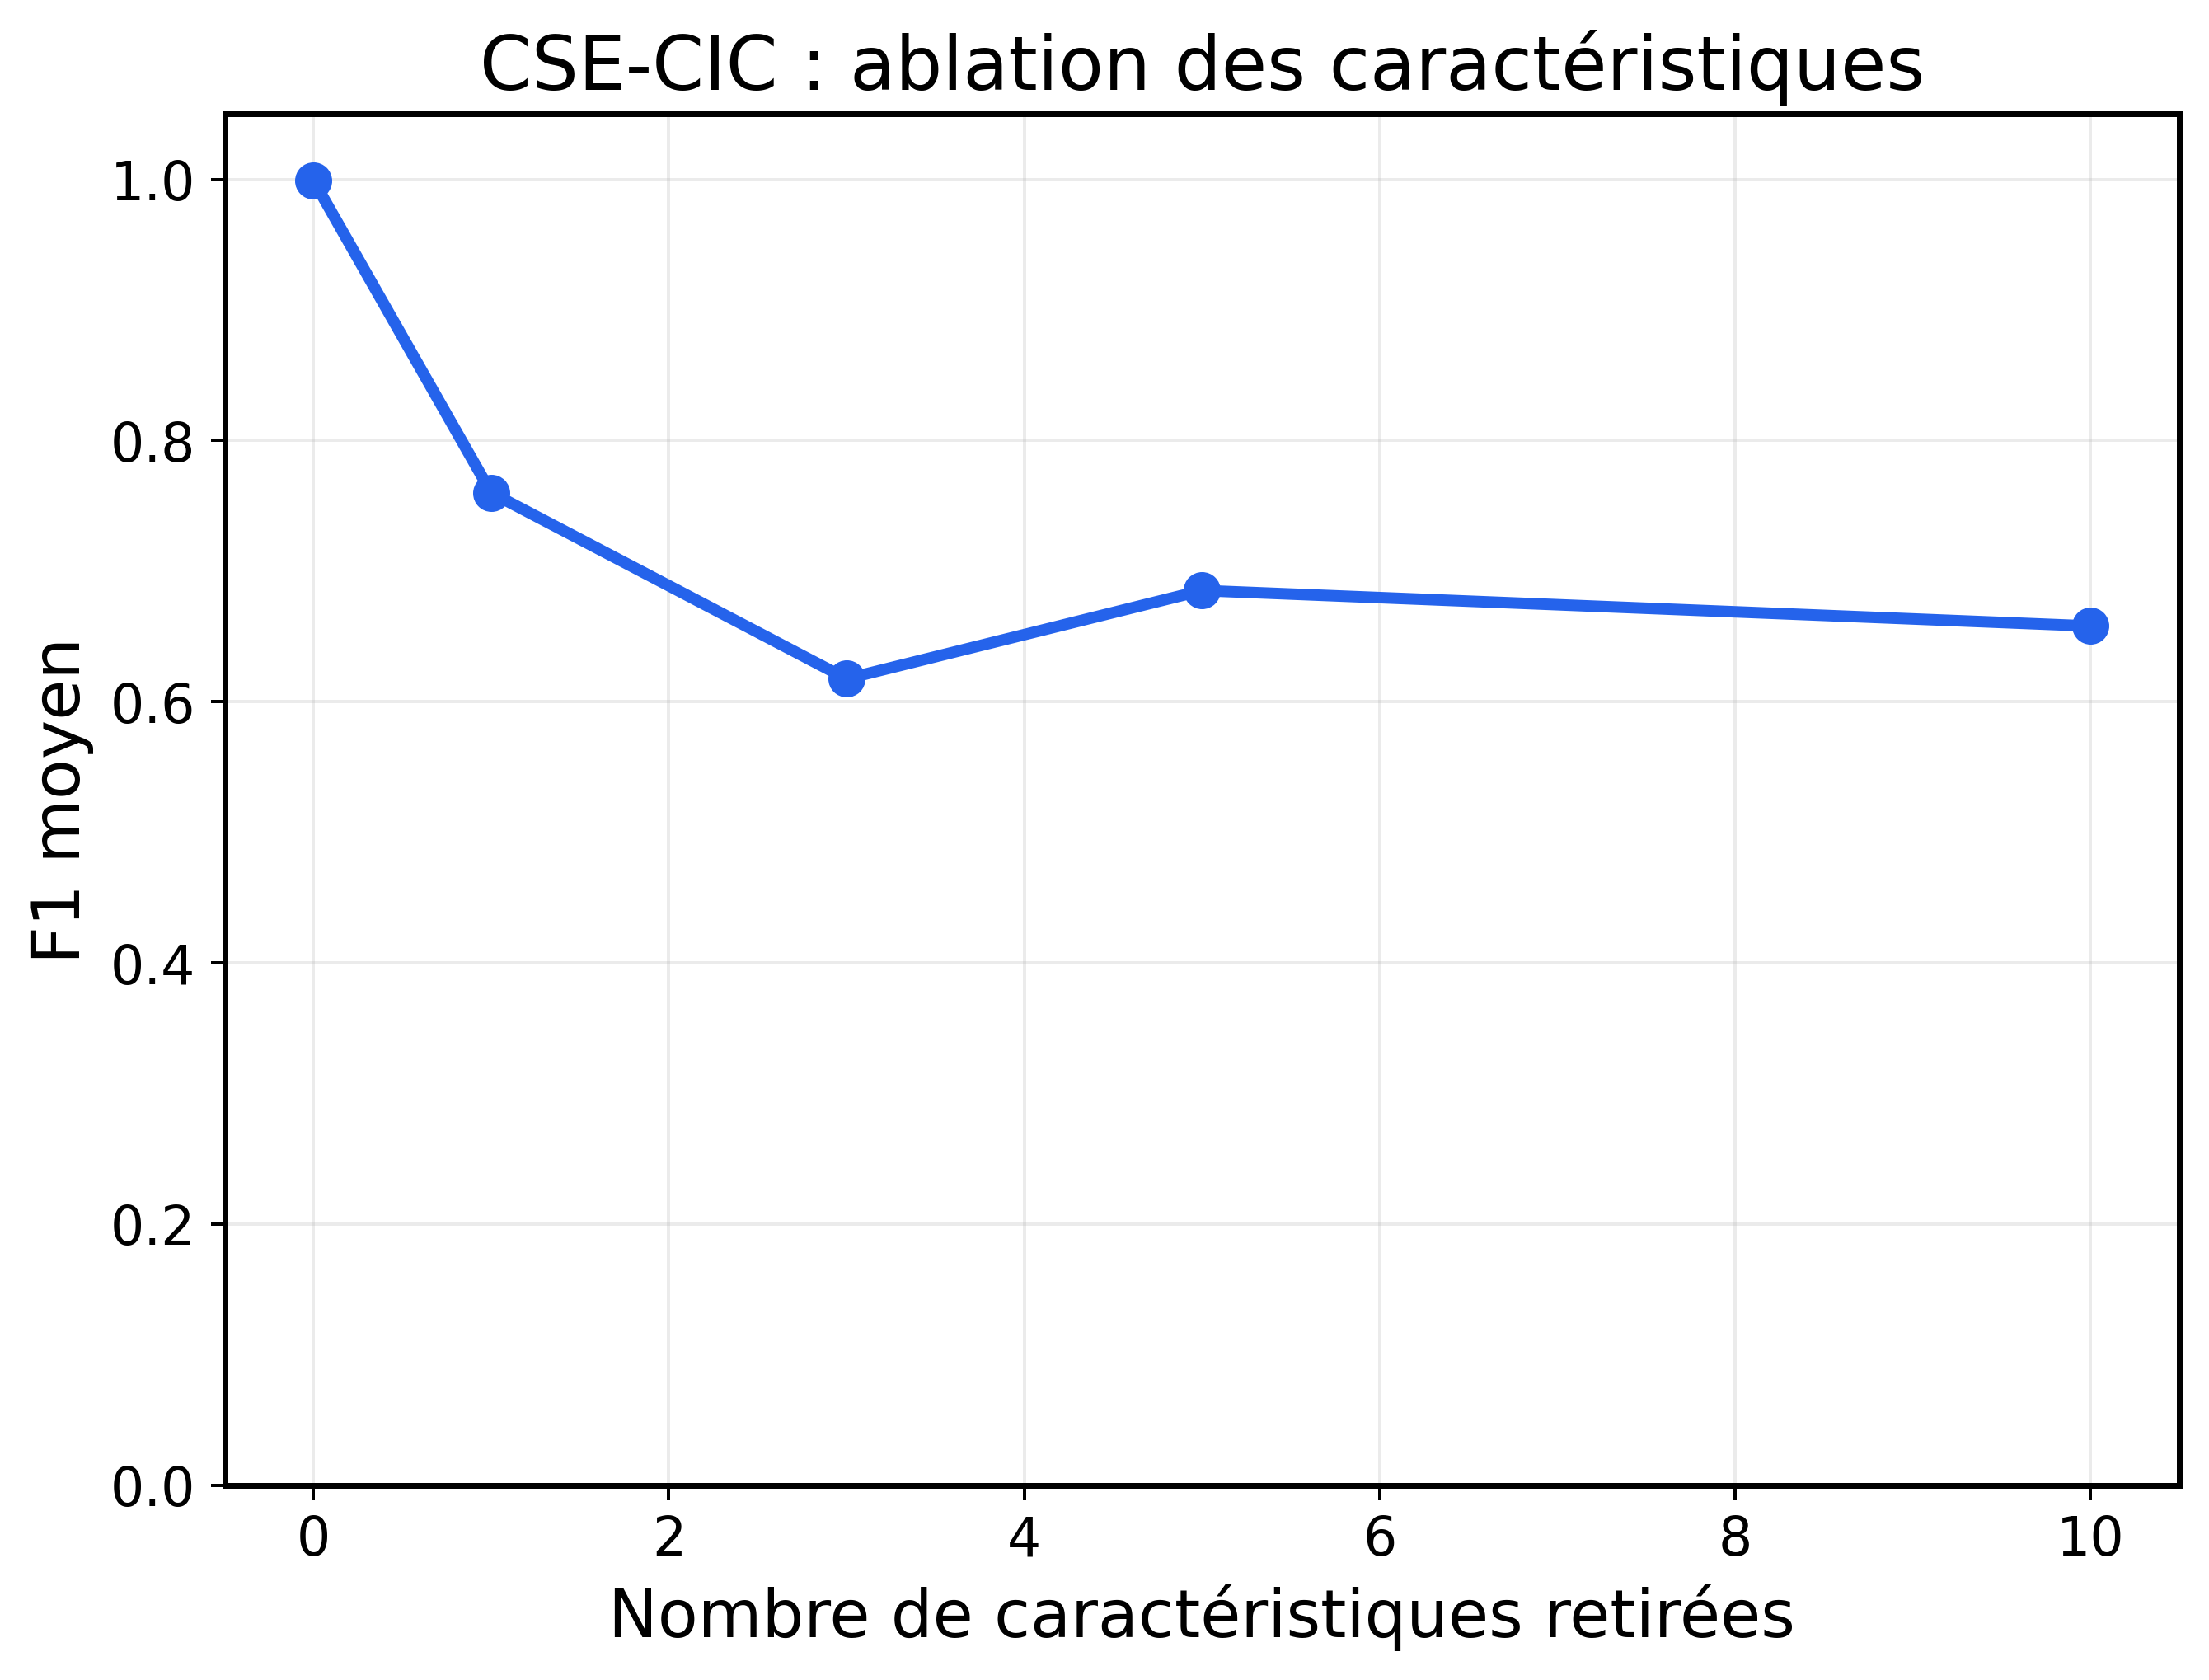
\includegraphics[width=0.80\textwidth]{figures/final/fig_csecic_lr_ablation.png}
\caption{Ablation CSE-CIC : évolution du F1 lorsque des caractéristiques sont retirées.}
\label{fig:csecic-ablation-final}
\end{figure}

\begin{figure}[H]
\centering
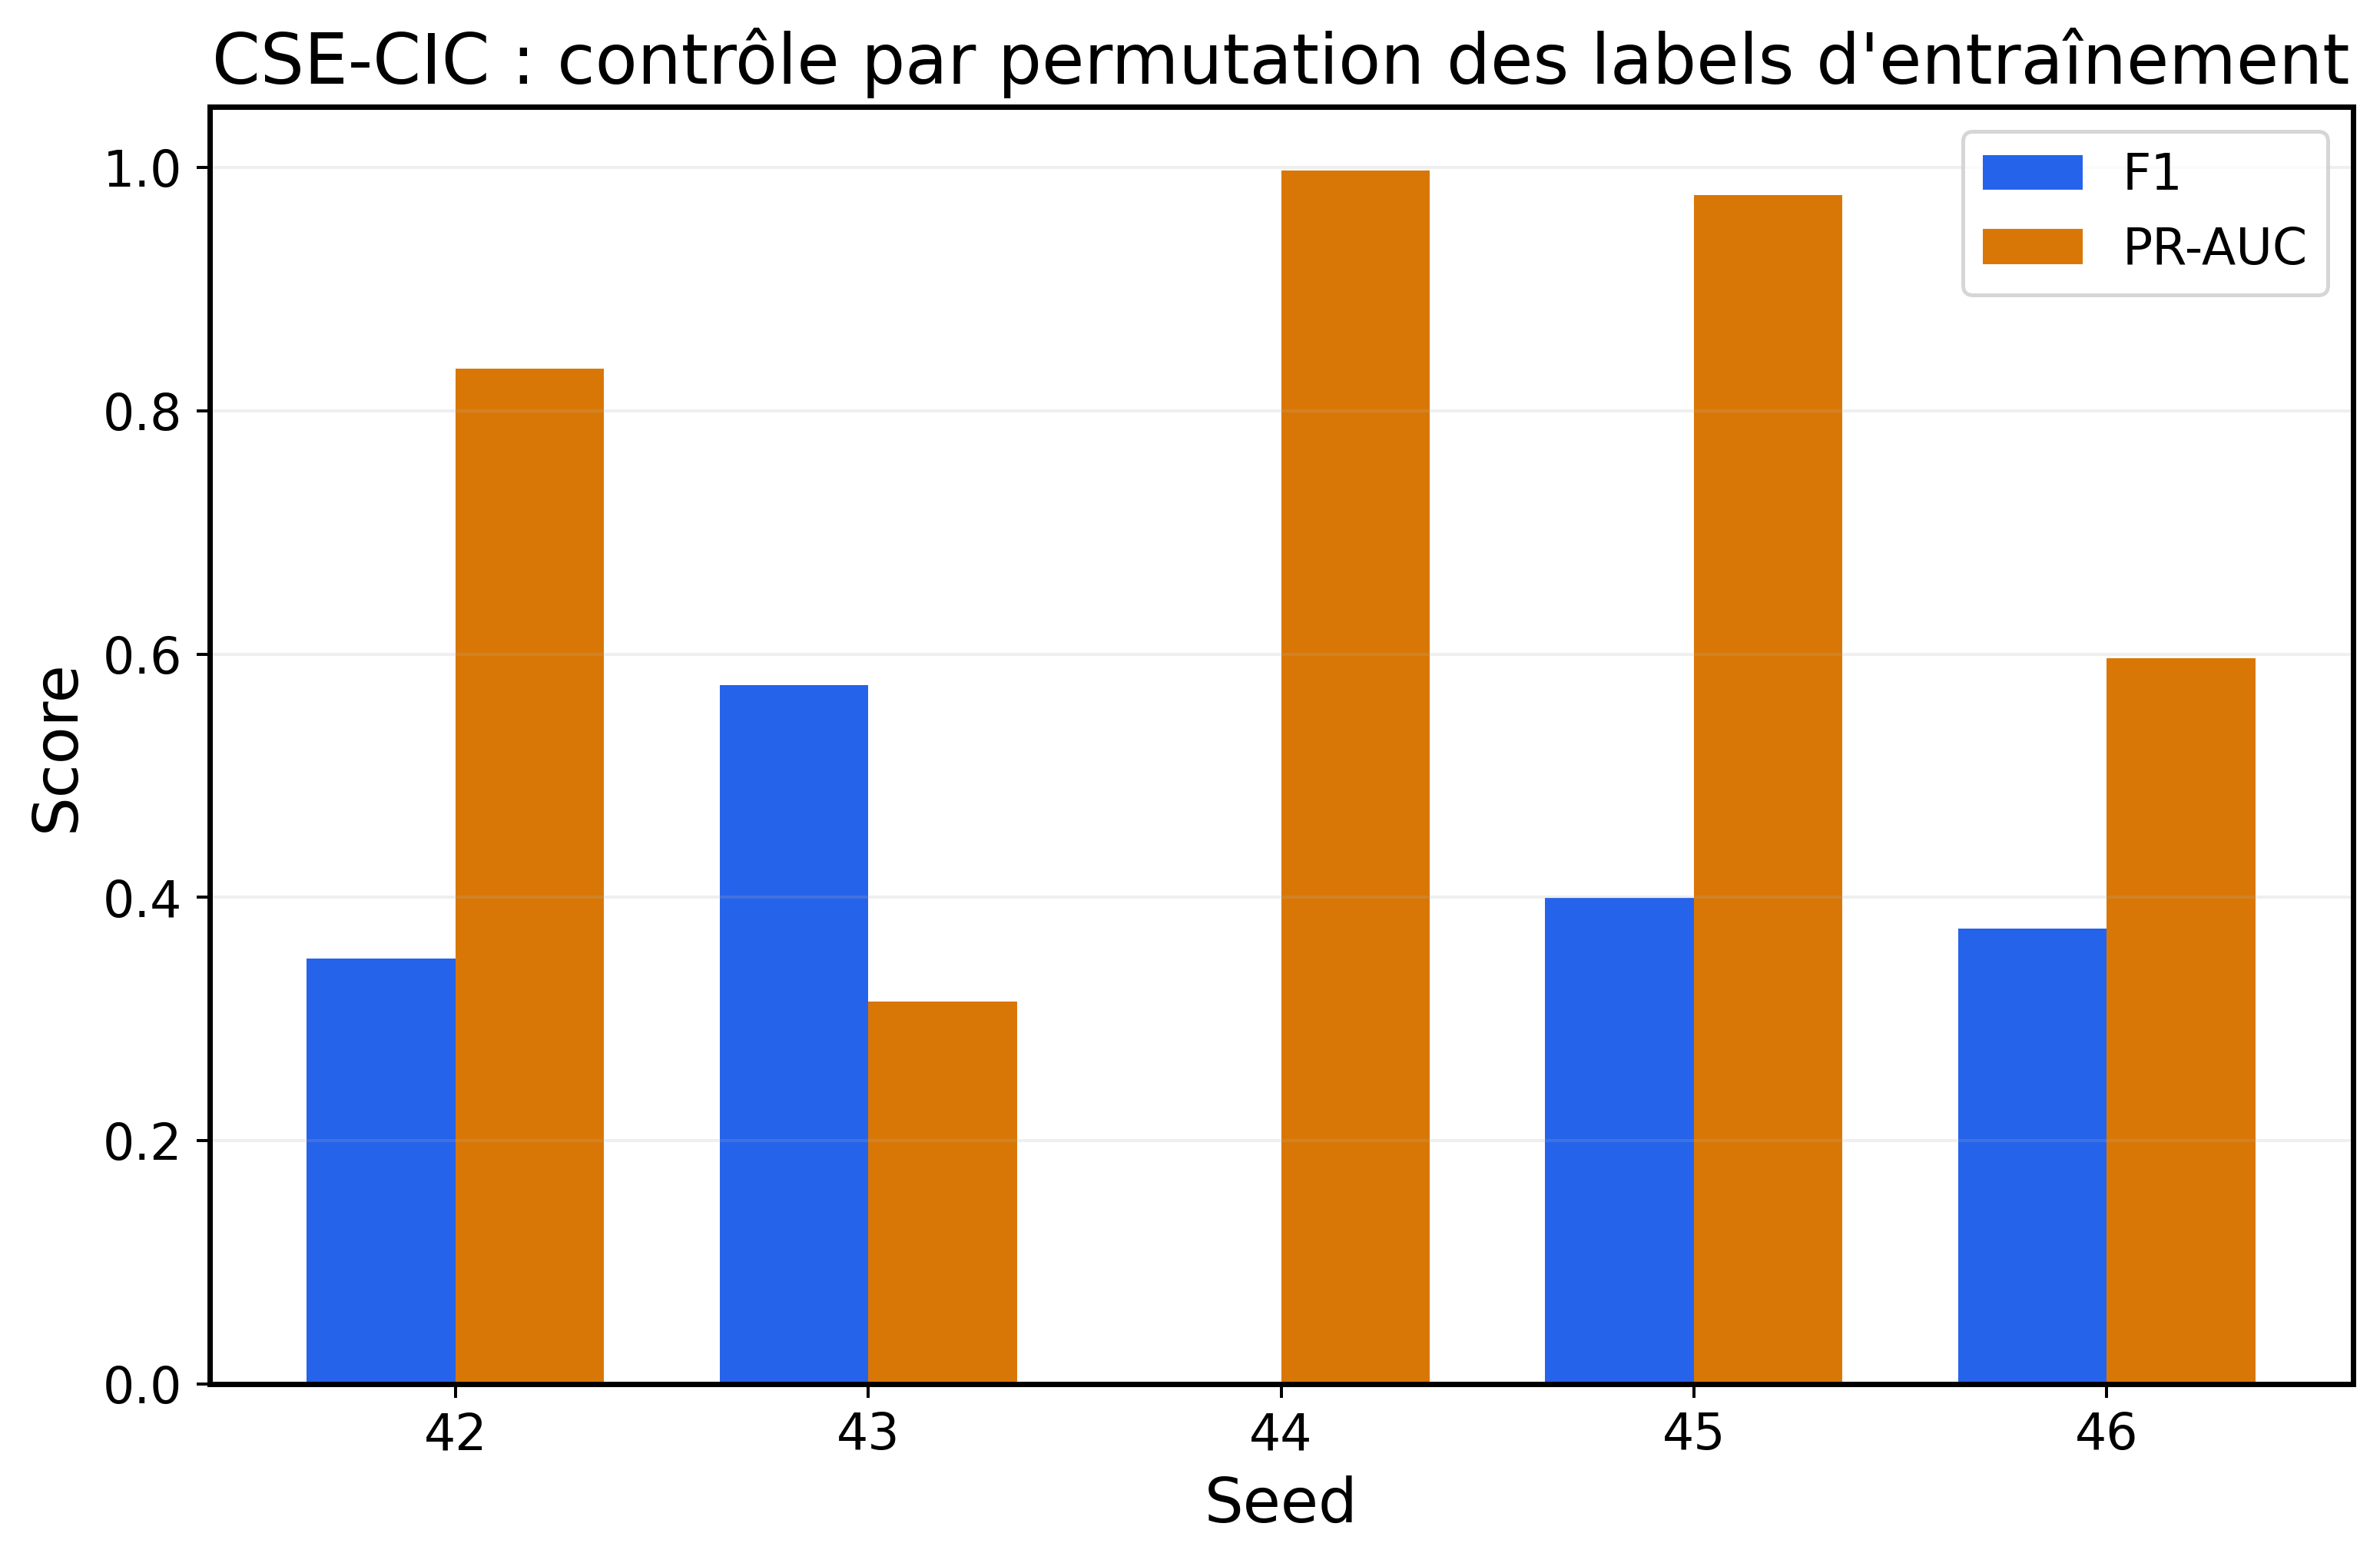
\includegraphics[width=0.88\textwidth]{figures/final/fig_csecic_lr_label_permutation.png}
\caption{Contrôle par permutation des labels d'entraînement sur les cinq seeds CSE-CIC.
La dispersion observée limite toute lecture naïve du score nominal.}
\label{fig:csecic-permutation-final}
\end{figure}

\section{Inférence réelle dans le pipeline CNP}

La campagne consolidée reprend 1\,401 unités et compare deux conditions. La condition H
utilise la règle légère historique ; la condition M charge l'artefact recommandé lorsqu'il
est compatible avec le schéma observé. Chaque trace conserve le modèle recommandé, le
modèle effectivement chargé, son hash, le marqueur d'inférence et le résultat de
l'exécution.

En condition H, les 1\,401 unités passent par la règle légère. En condition M, 1\,400
unités font l'objet d'une inférence réelle et une unité Apache utilise le fallback
heuristique explicitement enregistré. Aucune erreur ni réattribution n'est observée dans
ce run. La latence moyenne vaut $0{,}105420$~s en M, contre $0{,}031027$~s en H ; les
P95 correspondants sont $0{,}181044$~s et $0{,}068247$~s.

Les refus CNP sont des refus de capacité d'agents non compatibles avec certaines tâches et
ne sont pas des erreurs d'inférence. Une métrique prédictive globale n'est pas calculée.
Linux/auth est la seule source sélectionnée contenant les deux classes nécessaires à une
métrique descriptive : son F1 vaut $0{,}390244$. BGL et CICIDS ne comportent qu'une classe
dans les 200 premières unités retenues et restent donc \textbf{NON ÉVALUÉS} pour cette
métrique.

La campagne démontre la continuité fonctionnelle entre routage, résolution d'artefact,
chargement et inférence, au prix d'un coût temporel mesurable. Elle ne démontre ni un gain
prédictif systématique ni une accuracy multi-source globale.

\begin{figure}[H]
\centering
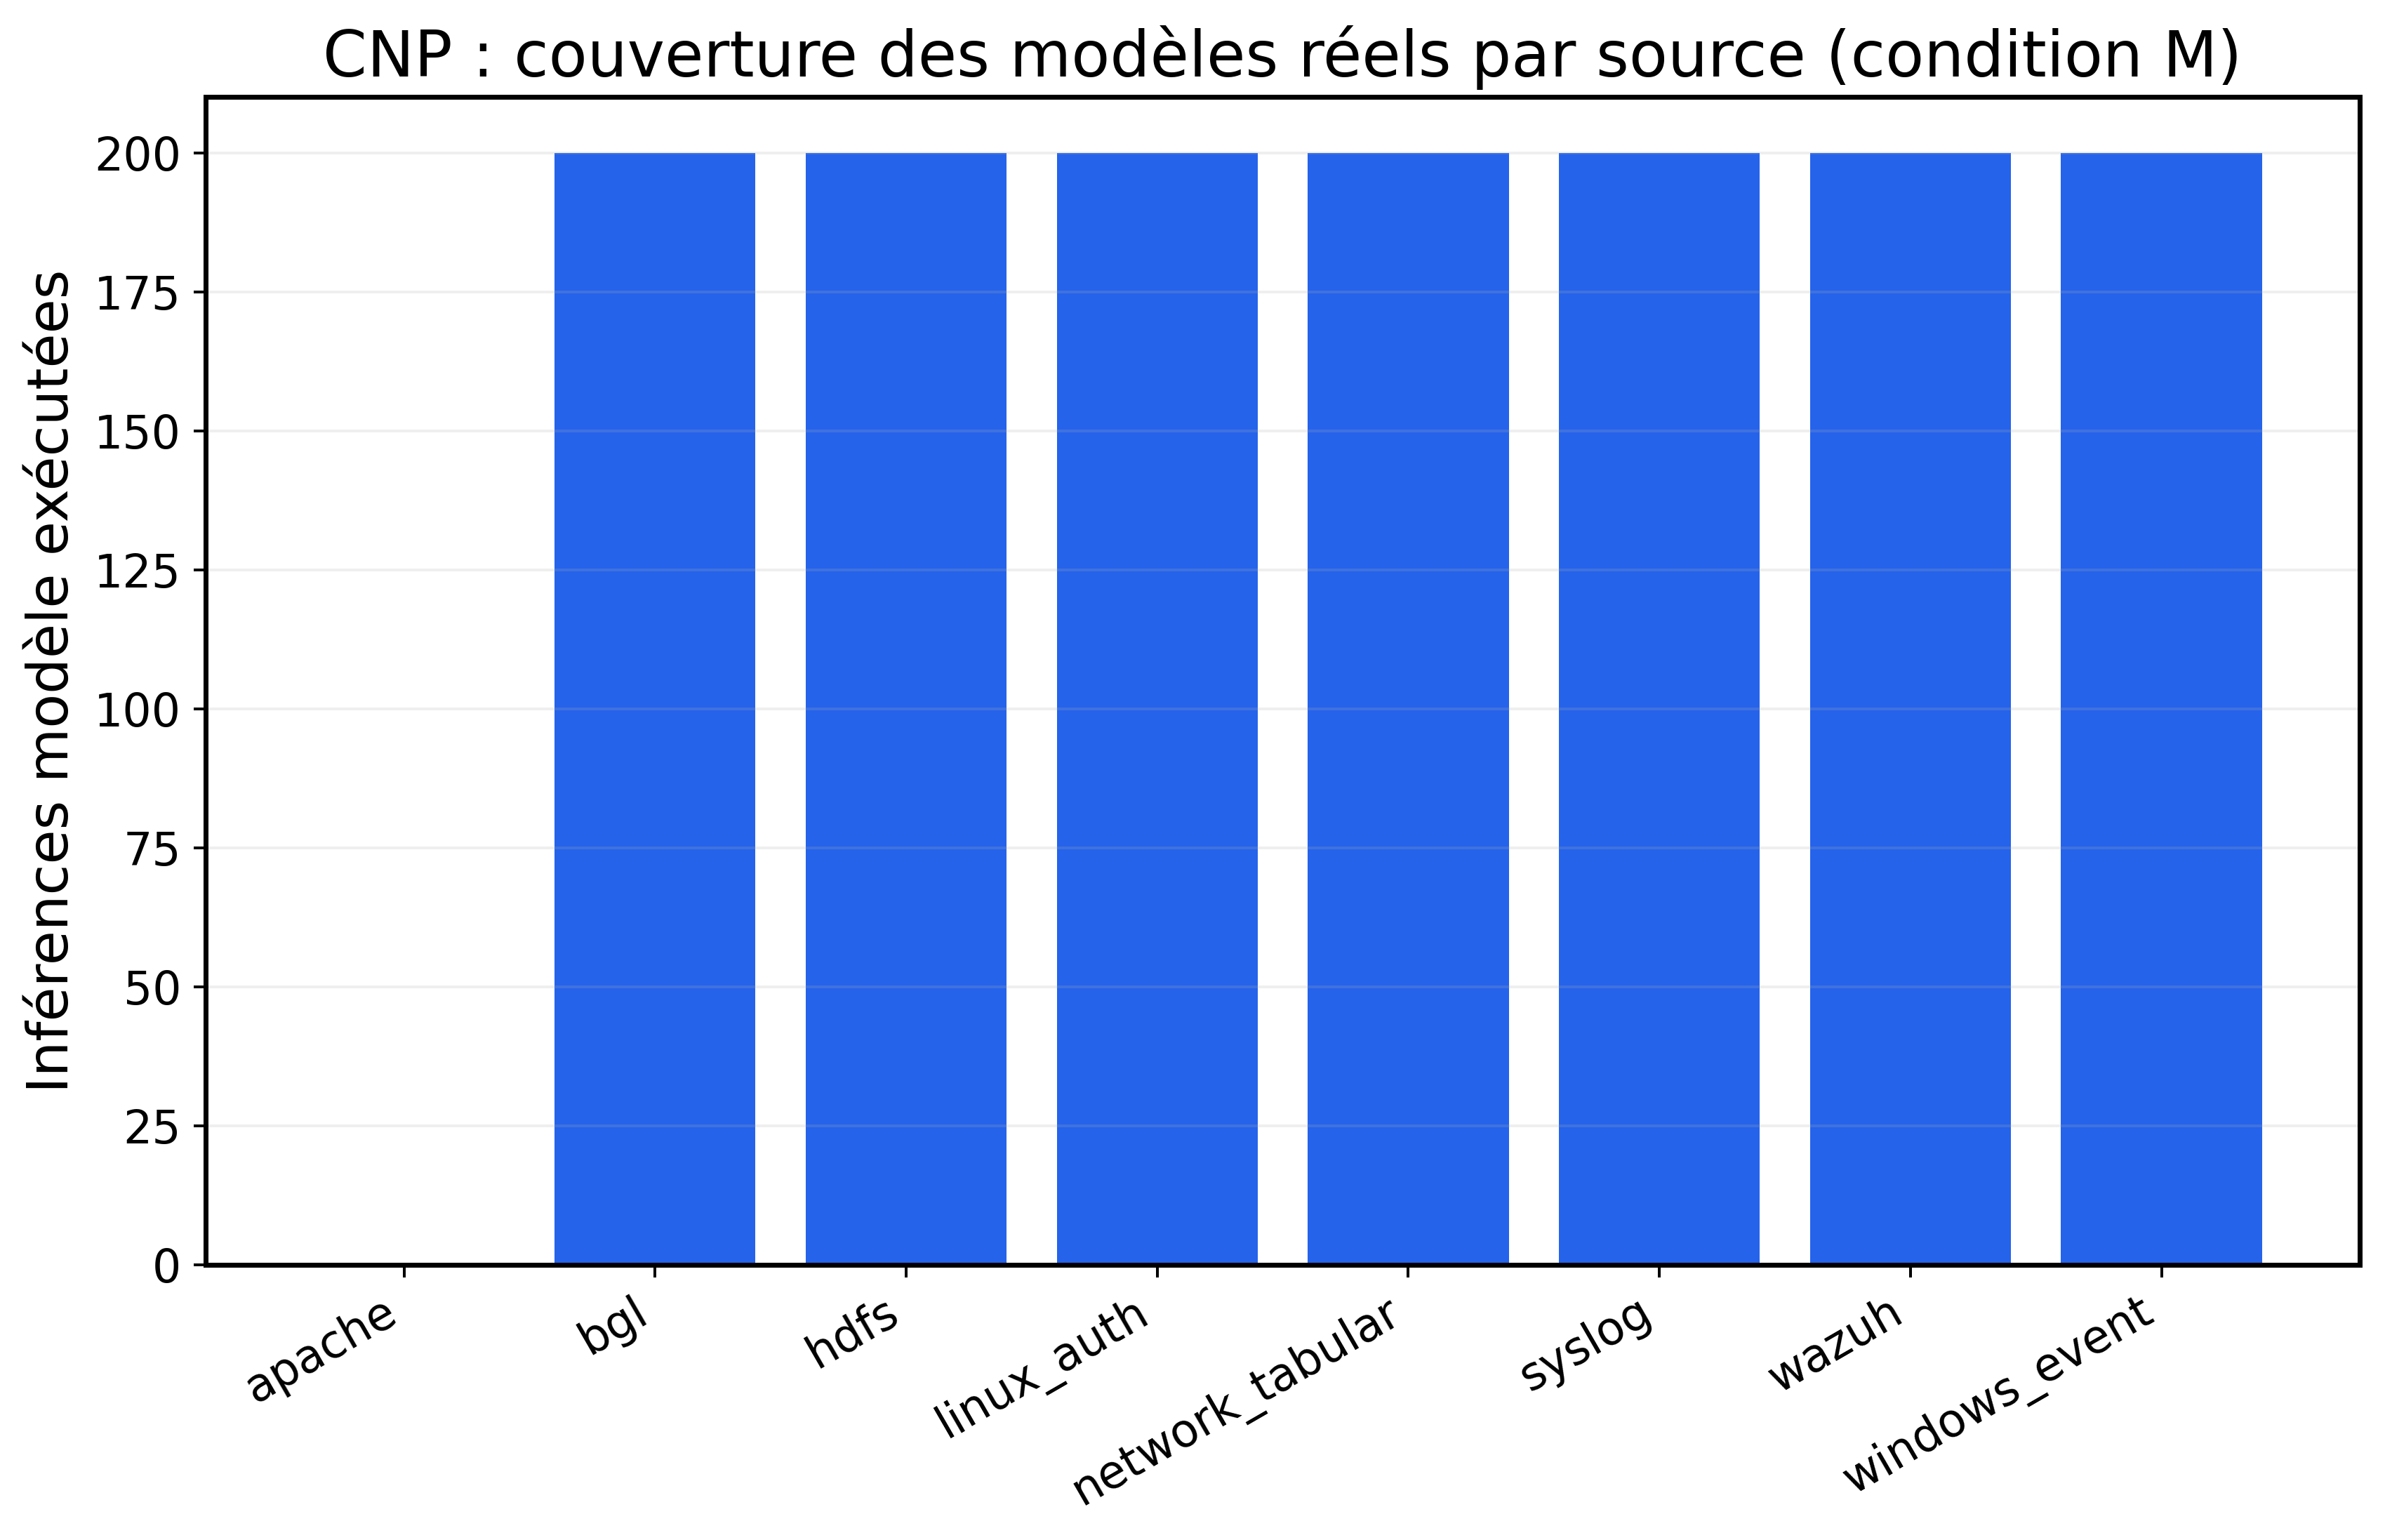
\includegraphics[width=0.94\textwidth]{figures/final/fig_e2e_real_model_coverage.png}
\caption{Couverture des inférences réelles par source dans la condition M du CNP. Les
1\,400 inférences réelles et l'unité Apache en fallback sont extraites de l'artefact final.}
\label{fig:e2e-real-coverage-final}
\end{figure}

\begin{figure}[H]
\centering
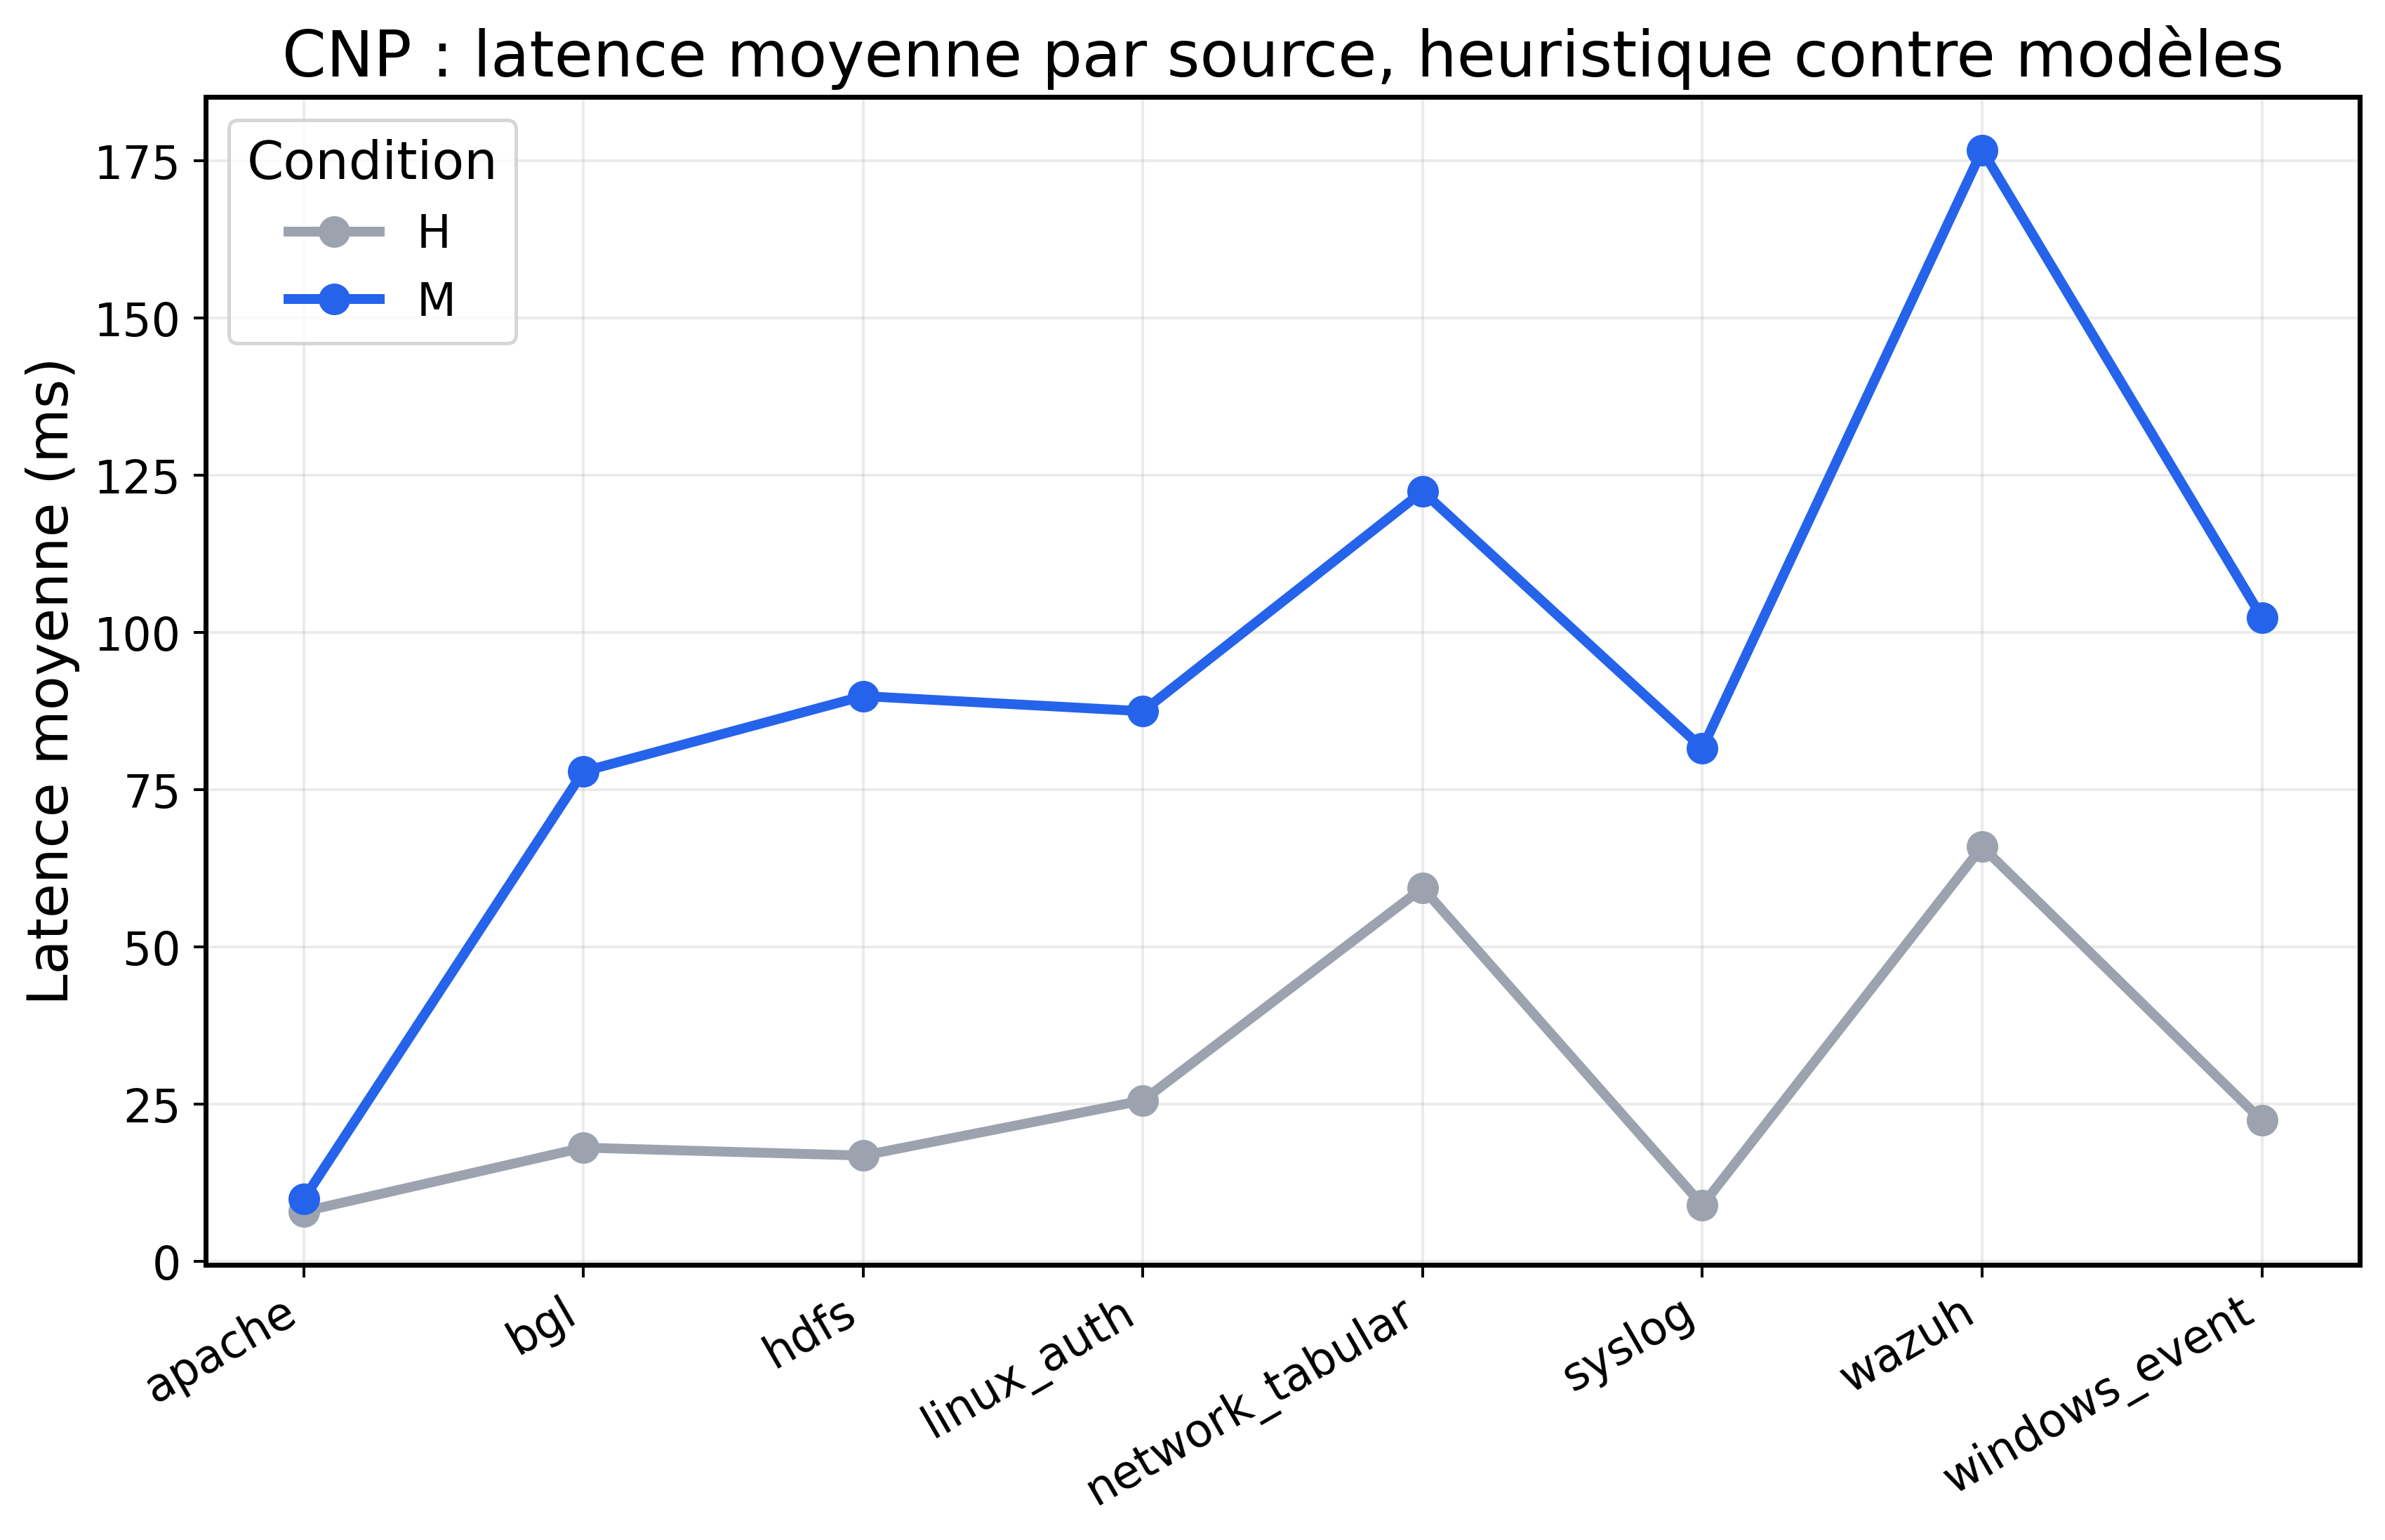
\includegraphics[width=0.94\textwidth]{figures/final/fig_e2e_real_model_latency.png}
\caption{Latence moyenne par source pour les conditions H (heuristique) et M (modèles
réels). La figure décrit le compromis de la campagne et non une garantie de production.}
\label{fig:e2e-real-latency-final}
\end{figure}

\section{Benchmark monolithique versus agents}

\subsection{Objectif}

La modularité d'une architecture multi-agent ne garantit pas qu'elle soit plus rapide.

Le benchmark contrôlé mesure explicitement le coût de cette orchestration.

Trois modes sont comparés sur :

\[
60 \text{ tâches}.
\]

Les modes sont :

\begin{enumerate}
    \item monolithe ;
    \item agents ;
    \item agents avec mécanisme de reprise.
\end{enumerate}

Les mesures principales sont :

\begin{itemize}
    \item durée ;
    \item débit ;
    \item CPU moyen ;
    \item RSS maximale.
\end{itemize}

Le CPU est exprimé en pourcentage d'un cœur logique équivalent.

La RSS est exprimée en MiB.

\subsection{Monolithe}

Le mode monolithique traite les 60 tâches en :

\[
36{,}6815~\mathrm{s}.
\]

Le débit est :

\[
1{,}6357~\mathrm{tâche/s}.
\]

Le CPU moyen atteint :

\[
121{,}339\,\%.
\]

La RSS maximale est :

\[
189{,}074~\mathrm{MiB}.
\]

\subsection{Agents}

Le mode agents traite les 60 tâches en :

\[
38{,}1803~\mathrm{s}.
\]

Le débit devient :

\[
1{,}5715~\mathrm{tâche/s}.
\]

Le CPU moyen est :

\[
165{,}746\,\%.
\]

La RSS maximale atteint :

\[
234{,}777~\mathrm{MiB}.
\]

\subsection{Agents avec reprise}

Le troisième mode termine également les 60 tâches.

La durée est :

\[
39{,}3000~\mathrm{s}.
\]

Le débit est :

\[
1{,}5267~\mathrm{tâche/s}.
\]

Le CPU moyen vaut :

\[
117{,}598\,\%.
\]

La RSS maximale est :

\[
189{,}395~\mathrm{MiB}.
\]

\subsection{Comparaison}

\begin{table}[H]
\centering
\caption{Benchmark contrôlé : monolithe versus architecture à agents}
\label{tab:benchmark-agents}
\small
\begin{tabular}{lrrrr}
\toprule
\textbf{Mode} &
\textbf{Durée (s)} &
\textbf{Tâches/s} &
\textbf{CPU moyen (\%)} &
\textbf{RSS max (MiB)} \\
\midrule
Monolithe & 36,6815 & 1,6357 & 121,339 & 189,074 \\
Agents & 38,1803 & 1,5715 & 165,746 & 234,777 \\
Agents + reprise & 39,3000 & 1,5267 & 117,598 & 189,395 \\
\bottomrule
\end{tabular}
\end{table}

La conclusion est claire :

\begin{quote}
\textit{À cette charge de 60 tâches, l'architecture à agents n'améliore pas le débit par
rapport au monolithe.}
\end{quote}

Ce résultat négatif doit être conservé.

\begin{figure}[H]
\centering
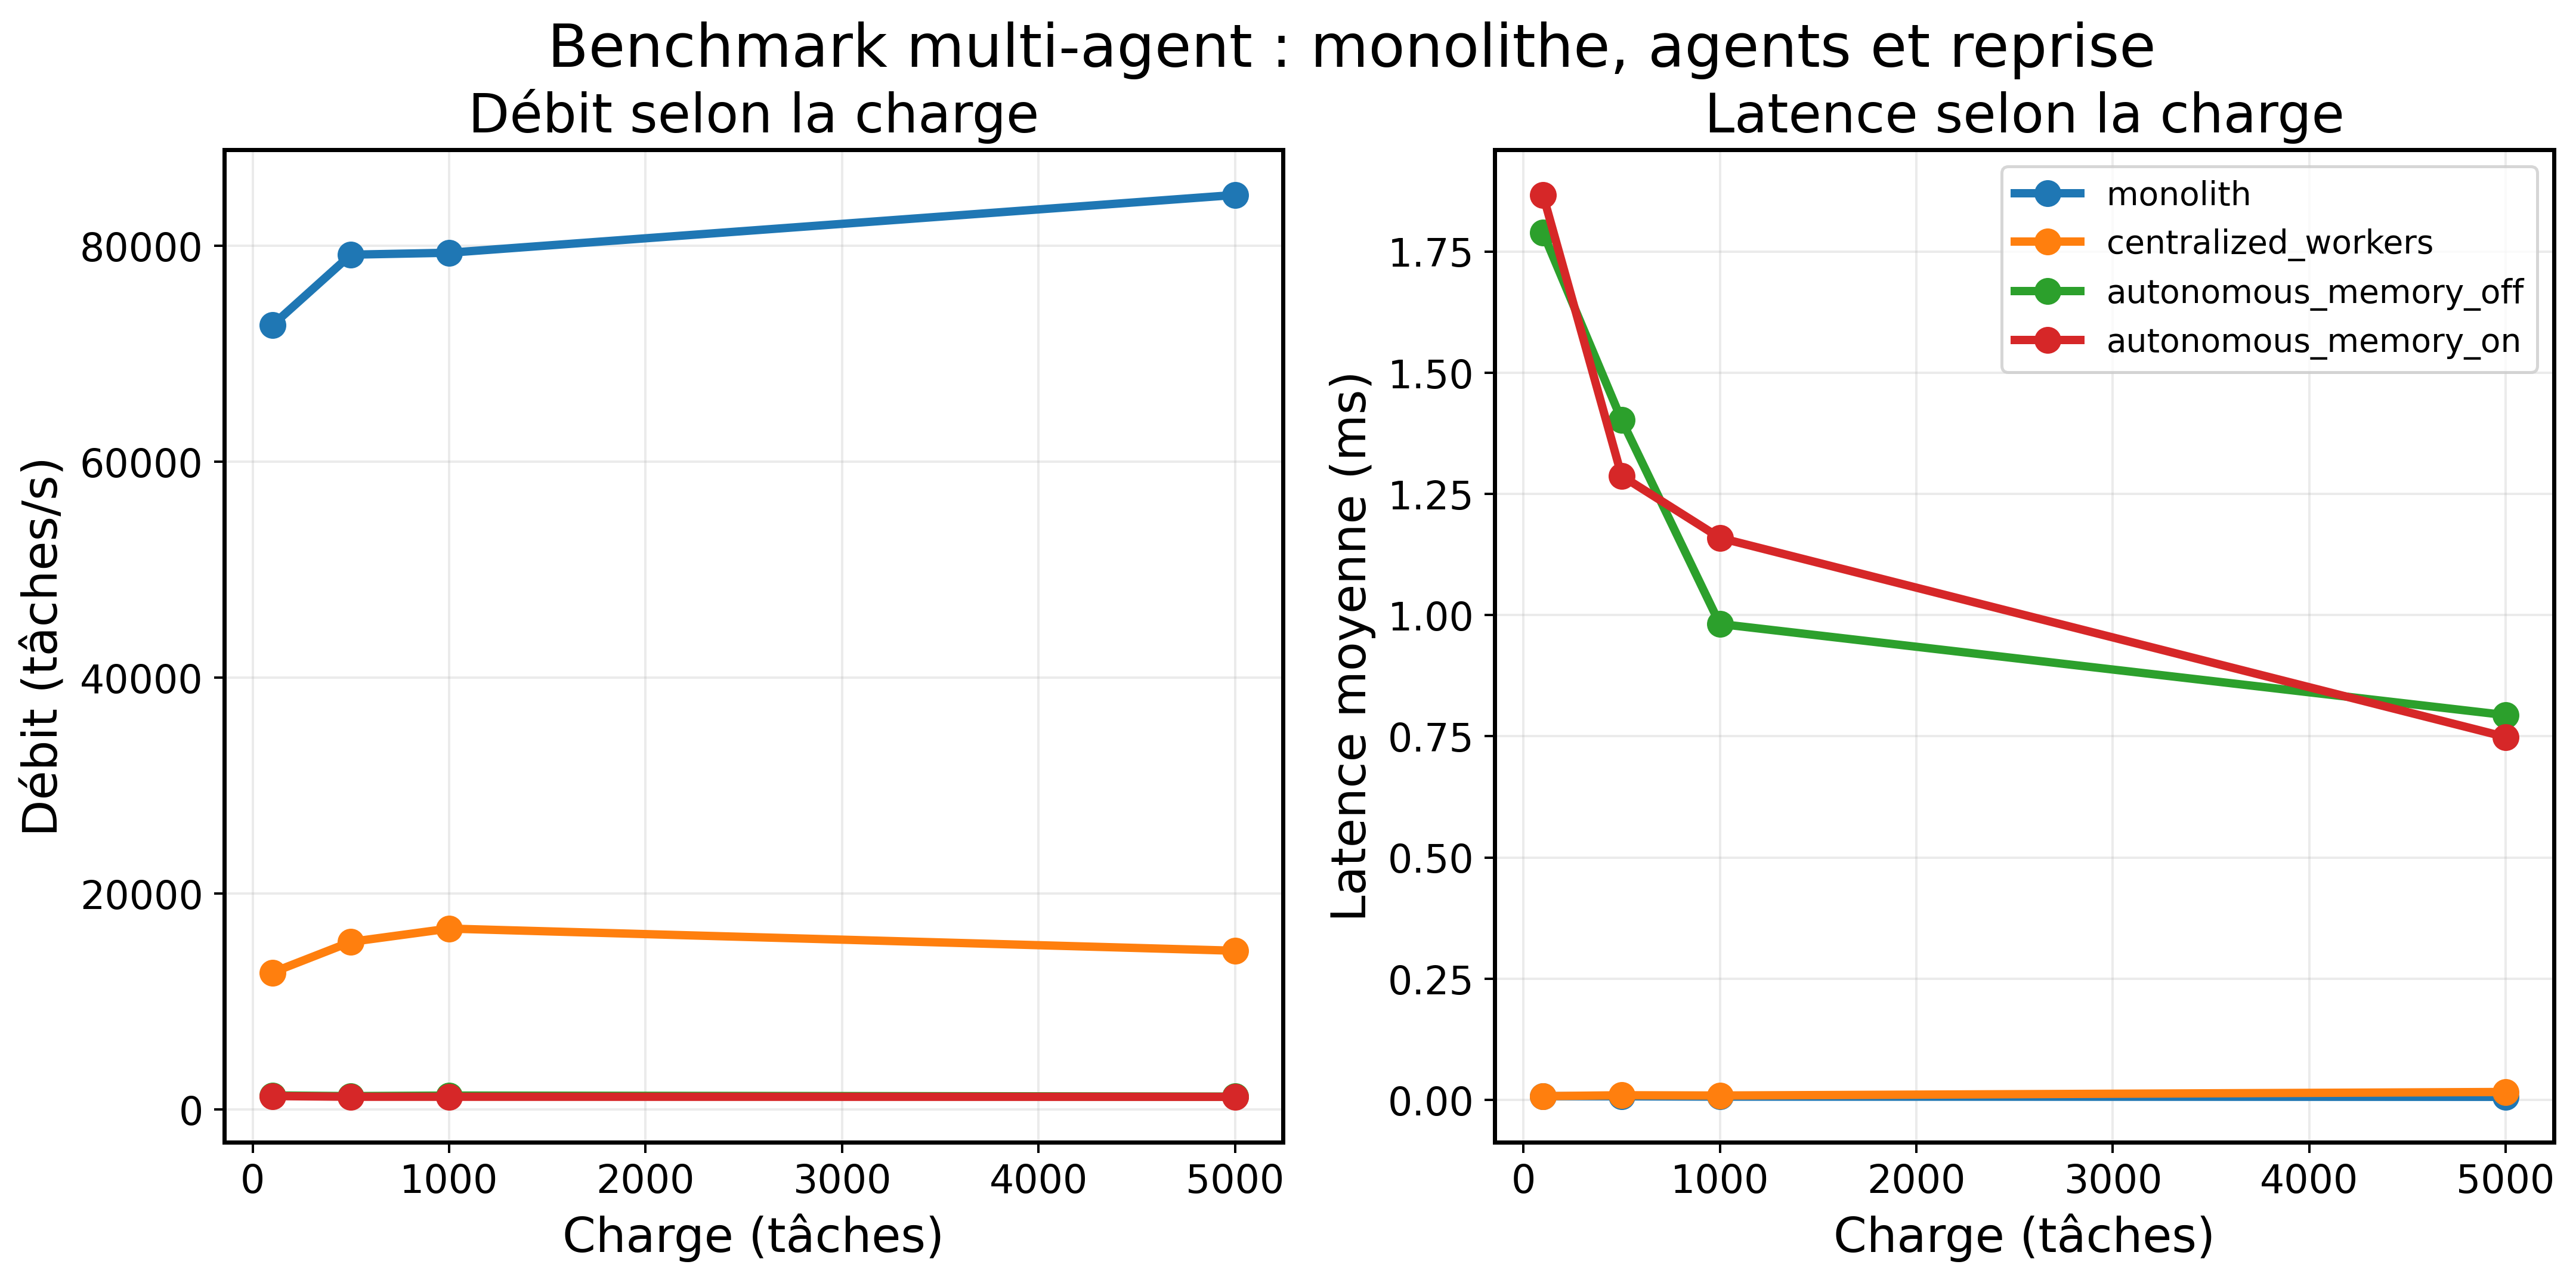
\includegraphics[width=0.96\textwidth]{figures/final/fig_multi_agent_throughput_latency.png}
\caption{Débit et latence du benchmark multi-agent (quatre architectures, quatre charges,
dix répétitions par configuration). Les unités de ressources associées aux tableaux sont
le pourcentage d'un cœur logique équivalent pour le CPU et la RSS en MiB.}
\label{fig:multi-agent-throughput-latency-final}
\end{figure}

Le bénéfice de l'architecture multi-agent doit plutôt être recherché dans :

\begin{itemize}
    \item la séparation des responsabilités ;
    \item la modularité ;
    \item l'audit ;
    \item la possibilité de distribuer certaines tâches ;
    \item les mécanismes de reprise étudiés.
\end{itemize}

Il serait incorrect de justifier l'architecture par une accélération qui n'est pas observée
dans le benchmark.

\section{Validation multi-VM}

\subsection{Objectif}

La campagne multi-VM vise à vérifier que plusieurs workers exécutés dans deux machines
virtuelles peuvent consommer des tâches placées dans un stream Redis commun.

L'expérience porte principalement sur le niveau transport et orchestration.

Elle ne cherche pas à reproduire un SOC industriel.

\subsection{Campagne multi-VM retenue}

La campagne principale retenue pour le mémoire est
\texttt{multivm\_cnp\_20260909T202632Z\_37592}. Elle exécute un agent Debian et un agent
Ubuntu, avec un Redis centralisé sur l'hôte Windows du laboratoire. Les deux machines
utilisent VirtualBox ; la durée exacte et les versions détaillées sont celles consignées
dans le manifeste de la campagne et ne sont pas extrapolées au-delà de cet environnement.

Le protocole soumet 60 tâches au réseau CNP, avec une répartition observée de 30 tâches
par VM. Les traces contiennent 15 messages \texttt{REFUSE}, un \texttt{FAIL} contrôlé suivi d'une
réattribution réussie et un replay idempotent exécuté par l'autre VM. Le replay ne produit
aucun effet dupliqué dans le registre contrôlé. Le résultat est donc $60/60$ tâches
terminées dans le scénario expérimenté.

Cette campagne démontre une négociation et une exécution multi-VM de laboratoire. Redis
reste un point central unique ; aucune haute disponibilité, tolérance aux partitions ou
montée en charge industrielle n'est évaluée.

\begin{figure}[H]
\centering
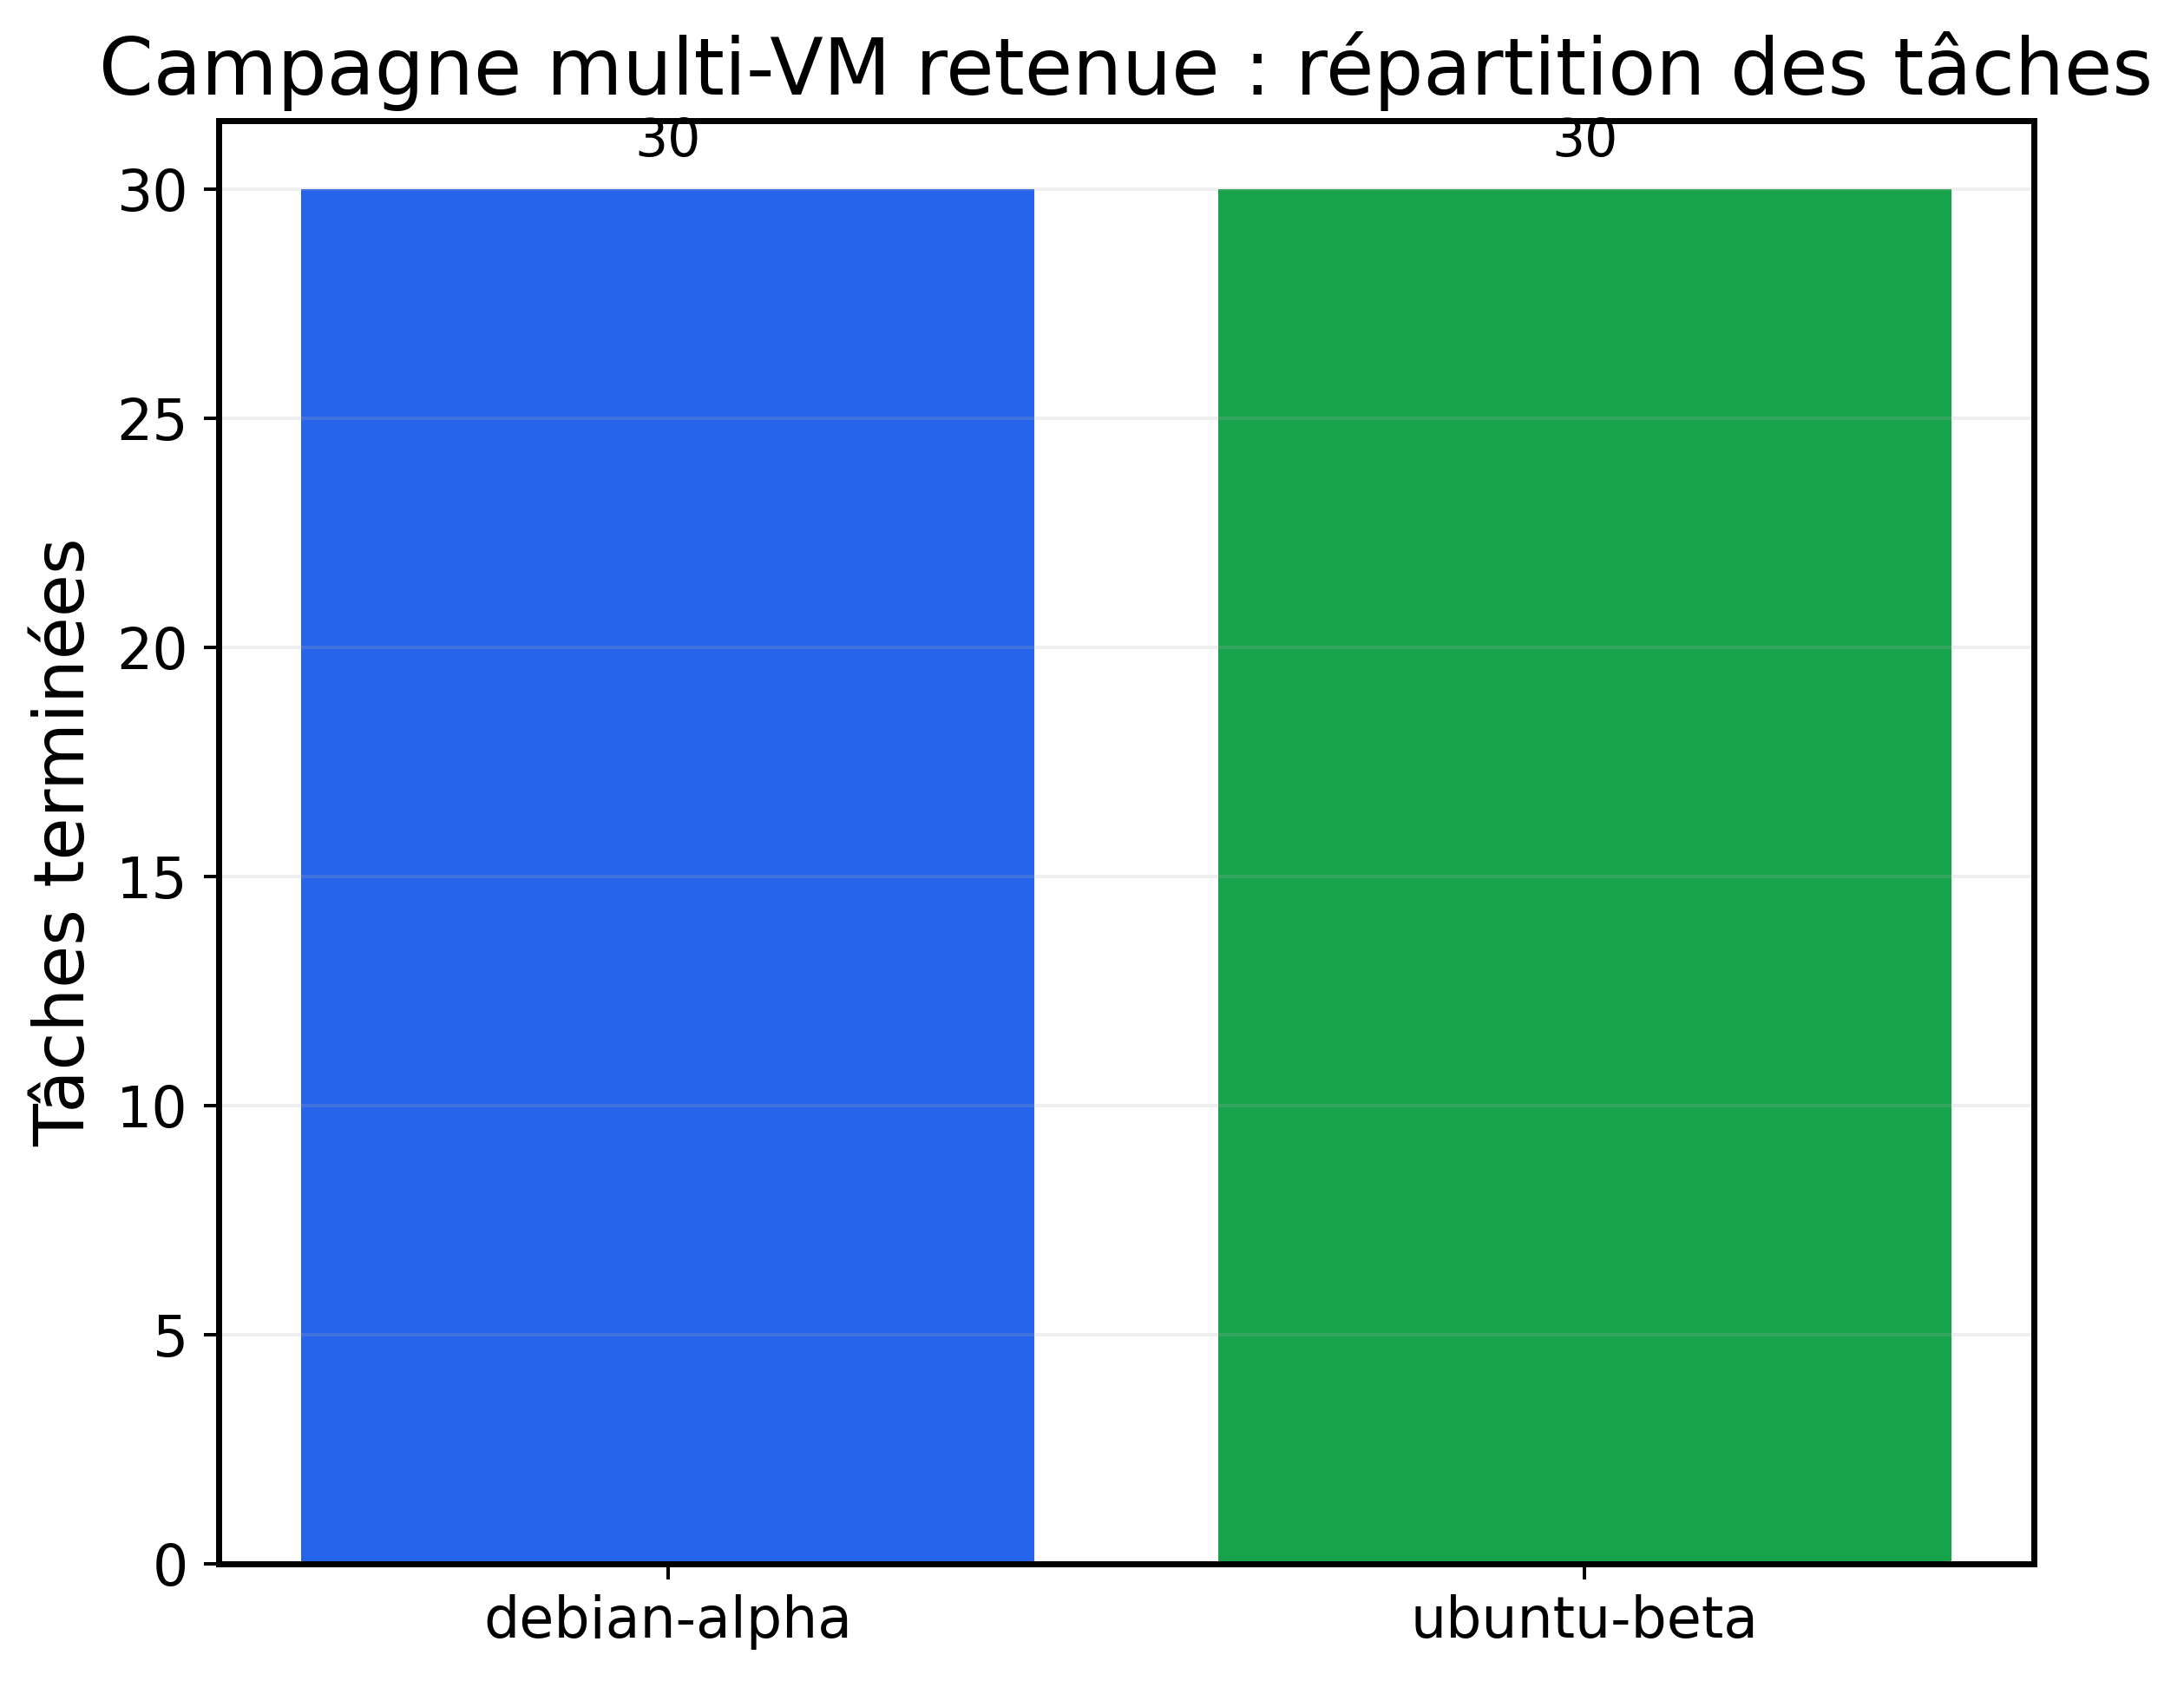
\includegraphics[width=0.72\textwidth]{figures/final/fig_multi_agent_task_distribution.png}
\caption{Répartition des 60 tâches de la campagne multi-VM retenue. Chaque VM traite 30
tâches ; les refus et la reprise contrôlée sont décrits dans le texte et le manifeste JSON.}
\label{fig:multi-vm-task-distribution-final}
\end{figure}

La campagne historique de 525 entrées lues et acquittées est conservée plus loin comme
contrôle de transport Redis. Elle ne remplace pas le run CNP retenu et ne doit pas être
interprétée comme 525 succès applicatifs.

\subsection{Configuration Redis}

Le service utilise :

\begin{itemize}
    \item image \texttt{redis:7-alpine} ;
    \item port 6379 ;
    \item AOF activé ;
    \item \texttt{appendfsync everysec} ;
    \item limite mémoire 512~MB ;
    \item politique \texttt{noeviction}.
\end{itemize}

\subsection{Run principal}

L'identifiant du run principal est :

\begin{verbatim}
redis-vbox-1h-20260722153650
\end{verbatim}

Le stream est :

\begin{verbatim}
logminer:agent_tasks:vbox_1h:20260722153650
\end{verbatim}

et le consumer group :

\begin{verbatim}
logminer-intelligent-agents
\end{verbatim}

Un worker est exécuté sur chaque VM.

Le parallélisme par worker est fixé à 1.

Les principaux paramètres sont :

\begin{itemize}
    \item \texttt{block-ms=1000} ;
    \item \texttt{claim-idle-ms=1000} ;
    \item durée configurée : 3\,720~s ;
    \item 120~s de drain incluses.
\end{itemize}

\subsection{Production des tâches}

Pendant la période cible, un lot de trois types de tâches est publié toutes les 15 secondes :

\begin{itemize}
    \item \texttt{discover.logs} ;
    \item \texttt{parse.logs} ;
    \item \texttt{route.model}.
\end{itemize}

La campagne observe :

\[
175 \text{ lots}.
\]

Chaque lot contient trois entrées, soit :

\[
175\times3=525.
\]

\subsection{Résultat principal}

Les 525 entrées sont :

\begin{itemize}
    \item enfilées ;
    \item lues ;
    \item acquittées par le consumer group.
\end{itemize}

À la fin :

\[
\mathrm{lag}=0,
\]

et :

\[
\mathrm{pending}=0.
\]

La formulation correcte est donc :

\begin{quote}
\textit{525 entrées ont été lues et acquittées par le groupe de consommateurs.}
\end{quote}

Il ne faut pas transformer ce constat en :

\begin{quote}
``525 tâches applicatives ont toutes réussi.''
\end{quote}

L'ACK mesure une propriété du transport et du consumer group.

\subsection{Relances}

Des interruptions liées au mécanisme de contrôle des invités VirtualBox ont nécessité des
relances supervisées.

Les identités de reprise incluent notamment :

\begin{verbatim}
debian-worker-1h-r2
ubuntu-worker-1h-r2
\end{verbatim}

Cette intervention humaine doit être conservée dans l'interprétation de la campagne.

\subsection{Campagne équilibrée}

Une campagne complémentaire :

\begin{verbatim}
redis-vbox-balanced-20260722145314
\end{verbatim}

porte sur 12 tâches uniques.

Le résultat enregistré est :

\[
12/12
\]

tâches terminées dans le protocole de cette campagne.

\subsection{Campagne de récupération}

Une troisième campagne :

\begin{verbatim}
redis-vbox-recovery-20260722150924
\end{verbatim}

teste un cas de reprise.

Une tâche est prise par Debian avant traitement/ACK puis reprise par Ubuntu.

La campagne termine avec :

\[
3/3
\]

tâches terminées et :

\[
\mathrm{pending}=0.
\]

Cette expérience démontre un scénario précis de récupération avant traitement/ACK.

Elle ne démontre pas :

\begin{itemize}
    \item la reprise après réussite métier mais avant ACK ;
    \item l'idempotence générale ;
    \item la reprise après interruption du serveur Redis ;
    \item la résistance aux partitions réseau ;
    \item la haute disponibilité de l'ensemble de l'architecture.
\end{itemize}

\subsection{Portée de la preuve}

La campagne multi-VM constitue une preuve de laboratoire de communication et de
consommation répartie.

Son infrastructure repose sur :

\begin{itemize}
    \item VirtualBox ;
    \item NAT ;
    \item Redis central unique ;
    \item interventions supervisées.
\end{itemize}

Ces conditions sont suffisantes pour démontrer le mécanisme étudié, mais pas pour soutenir
une revendication de déploiement distribué industriel.

\section{Corrélation synthétique contrôlée}

\subsection{Pourquoi un corpus séparé}

Évaluer un corrélateur nécessite une vérité terrain différente de celle utilisée pour
évaluer un classifieur.

Il faut savoir quelles paires d'anomalies doivent appartenir au même incident.

Un corpus synthétique est donc construit afin que cette vérité soit connue indépendamment
du moteur.

\subsection{Composition}

Le corpus contient :

\[
19 \text{ événements}.
\]

Parmi eux :

\[
16 \text{ anomalies}
\]

sont associées à :

\[
6 \text{ incidents vrais},
\]

et :

\[
3 \text{ événements de bruit}
\]

complètent le scénario.

La vérité de regroupement est enregistrée dans un fichier distinct qui n'est pas fourni au
corrélateur comme entrée.

\subsection{Paramètres}

La fenêtre temporelle fixe est :

\[
15 \text{ minutes}.
\]

Huit clés réelles de corrélation sont utilisées.

Le corpus comprend volontairement plusieurs situations :

\begin{itemize}
    \item groupes stables ;
    \item séparation par hôte ;
    \item incident traversant une frontière horaire ;
    \item deux incidents distincts impossibles à distinguer avec les seules clés retenues ;
    \item bruit.
\end{itemize}

\subsection{Évaluation pairwise}

Avec 16 anomalies, le nombre de paires possibles est :

\[
\binom{16}{2}
=
120.
\]

Chaque paire peut être classée selon que les deux événements doivent ou non appartenir au
même incident.

Les résultats sont :

\[
\mathrm{Precision}=0{,}764706,
\]

\[
\mathrm{Recall}=0{,}866667,
\]

\[
F_1=0{,}812500.
\]

\subsection{Modes d'échec}

Deux modes d'échec sont particulièrement importants.

Le premier est la \textbf{fragmentation} : des événements appartenant à un même incident
vrai se retrouvent séparés.

Le second est la \textbf{fusion} : deux incidents distincts sont réunis.

Le corpus final contient au moins un exemple de chacun de ces comportements.

Ce résultat montre qu'obtenir un nombre plausible d'incidents ne suffit pas pour conclure
que la corrélation est correcte. La structure interne des groupes doit également être
évaluée.

\subsection{Portée}

La conclusion permise est :

\begin{quote}
\textit{Le corrélateur a été évalué sur des scénarios synthétiques contrôlés avec un
F1 pairwise de 0,812500.}
\end{quote}

Cette expérience n'est pas une validation sur incidents SOC réels annotés.

\IfFileExists{figures/correlation_synthetic_metrics.png}{
\begin{figure}[H]
\centering

\includegraphics[width=0.76\textwidth]{figures/correlation_synthetic_metrics.png}
\caption{Métriques de la corrélation sur le corpus synthétique contrôlé.}
\label{fig:correlation}
\end{figure}

\begin{center}
\footnotesize Source : auteur, à partir des résultats expérimentaux de ce travail.
\end{center}
}{}

\section{Synthèse transversale des expériences}

Le tableau~\ref{tab:synthese-resultats-finaux} rassemble les résultats principaux.

\begin{table}[H]
\centering
\caption{Synthèse des principaux résultats expérimentaux}
\label{tab:synthese-resultats-finaux}
\scriptsize
\begin{tabularx}{\textwidth}{p{3cm}p{4.2cm}X}
\toprule
\textbf{Expérience} &
\textbf{Résultat principal} &
\textbf{Interprétation} \\
\midrule

CICIDS random &
$F_1=0{,}995142\pm0{,}001013$, $N=5$. &
Performance élevée dans une séparation aléatoire stratifiée ; ne prouve pas la
généralisation hors scénario. \\

CICIDS holdout &
F1 macro $=0{,}157744$. &
Forte sensibilité aux scénarios exclus de l'entraînement. \\

Cinq modèles &
LR : F1 macro $0{,}233670$ ; HGB : PR-AUC macro $0{,}567697$. &
Aucun candidat ne domine toutes les métriques ni ne résout la fragilité générale. \\

HDFS block-level &
Histogram : F1 $0{,}892308$, 29 positifs ; bootstrap médiane $0{,}894737$. &
Résultat observé sur 2\,000 blocs ; intervalle descriptif variable et aucune indépendance revendiquée. \\

BGL strict &
Histogram : F1 $0{,}913698$, FPR $0{,}032016$, $N=1$. &
Bonne séparabilité observée, avec fort déplacement de templates. \\

Mise à jour &
$\Delta=+0{,}067845$, $-0{,}063163$, $+0{,}009016<0{,}02$. &
Les trois branches de gouvernance sont fonctionnelles. \\

Multiformat &
7\,001 lues, parsées et normalisées sur 7\,001. &
Couverture de pipeline complète pour cette campagne ; la complétude des champs reste
variable selon l'adaptateur. \\

Routeur &
80/81 ; accuracy $0{,}987654$ ; F1 macro $0{,}883598$. &
Très bonne attribution dans le corpus dérivé ; portée externe limitée. \\

Monolithe/agents &
1,6357 contre 1,5715 tâche/s. &
À 60 tâches, les agents n'améliorent pas le débit. \\

Multi-VM CNP &
60/60 tâches ; Debian/Ubuntu 30/30 ; 15 refus ; 1 échec contrôlé ; 1 réattribution. &
Négociation et reprise idempotente démontrées en laboratoire avec Redis central. \\

Corrélation &
Precision $0{,}764706$, recall $0{,}866667$, F1 $0{,}812500$. &
Validation synthétique contrôlée ; fragmentation et fusion restent possibles. \\

\bottomrule
\end{tabularx}
\end{table}

\section{Résultats positifs et résultats négatifs}

Une lecture scientifique du chapitre ne doit pas retenir uniquement les valeurs les plus
élevées.

Plusieurs résultats positifs sont clairement établis :

\begin{itemize}
    \item le protocole aléatoire CICIDS est reproductible sur cinq seeds ;
    \item le routeur attribue correctement 80 des 81 fichiers du corpus dérivé ;
    \item la mise à jour contrôlée exécute effectivement les trois décisions prévues ;
    \item la campagne CNP multi-VM termine 60/60 tâches avec une réattribution contrôlée ;
    \item la corrélation obtient un F1 pairwise supérieur à 0,8 dans son corpus synthétique ;
    \item BGL présente une bonne séparabilité dans le protocole strict retenu.
\end{itemize}

Mais les résultats négatifs sont tout aussi informatifs :

\begin{itemize}
    \item les holdouts CICIDS révèlent plusieurs F1 nuls ou presque nuls ;
    \item aucun des cinq modèles ne résout le scénario Bot ;
    \item HDFS conserve un F1 faible dans le protocole strict ;
    \item HDFS et BGL ne sont pas normalisés par la voie multiformat générale ;
    \item le routage spécialisé n'apporte pas systématiquement un gain prédictif ;
    \item les agents réduisent légèrement le débit dans le benchmark contrôlé ;
    \item le corrélateur produit à la fois fragmentation et fusion dans certains cas.
\end{itemize}

Ces résultats évitent de présenter Ariel \logminer{} comme une architecture dont toutes les
composantes seraient déjà optimales.

Ils indiquent plutôt quelles parties du prototype sont démontrées, lesquelles restent
partielles et où se situent les principaux axes d'amélioration.

\section{Réponse expérimentale préliminaire aux questions de recherche}

À ce stade, les résultats permettent déjà d'associer chaque question de recherche à un
ensemble de preuves, sans encore procéder à la discussion complète.

\subsection*{QR1 --- Normalisation}

La validation multiformat lit, parse et normalise 7\,001 unités sur 7\,001 dans la campagne
finale. La couverture des champs et la conservation exacte du brut restent toutefois
dépendantes de l'adaptateur.

La réponse est donc nécessairement partielle.

\subsection*{QR2 --- Architecture multi-agent}

Le code et les campagnes Redis démontrent une organisation par agents, des consumer groups,
des ACK et un scénario de reprise.

Le benchmark montre cependant que cette architecture n'améliore pas le débit à la charge
testée.

La modularité et la traçabilité sont soutenues, tandis que la robustesse industrielle
reste hors du périmètre.

\subsection*{QR3 --- Sélection automatique}

Le routeur historique obtient 80/81 sur son corpus dérivé ; le contrôle open-set consolidé
rejette 3/3 fichiers inconnus sans faux rejet parmi 28 fichiers connus.

L'ablation montre en parallèle que cette bonne attribution ne conduit pas à un gain
prédictif systématique.

La fonction de sélection est donc démontrée dans le corpus, mais sa valeur prédictive
générale ne l'est pas.

\subsection*{QR4 --- Dashboard}

Le dashboard permet l'affichage et l'inspection fonctionnelle des résultats.

Aucune étude utilisateur n'est cependant menée.

Les expériences du présent chapitre n'établissent donc pas une amélioration mesurée de
l'utilisabilité.

\subsection*{QR5 --- Mémoire et mise à jour}

La mémoire et l'audit existent dans le prototype.

La procédure de mise à jour contrôlée est exécutée de bout en bout avec une promotion et
deux rejets.

Le bénéfice causal de la mémoire sur la qualité de priorisation n'est toutefois pas isolé.

\subsection*{QR6 --- Évaluation}

Les campagnes associent :

\begin{itemize}
    \item métriques ;
    \item seeds ;
    \item splits ;
    \item mesures CPU/RAM ;
    \item manifestes ;
    \item hashes ;
    \item fichiers CSV/JSON ;
    \item expériences de transport ;
    \item artefacts de figures.
\end{itemize}

Dans le périmètre du prototype, cette question reçoit la réponse expérimentale la plus
solide.

\section{Limites immédiates des résultats}

Les limites détaillées feront l'objet du chapitre suivant. Plusieurs doivent néanmoins être
rappelées ici afin que les valeurs précédentes ne soient pas surinterprétées.

Pour CICIDS2017, l'échantillonnage est plafonné et la lecture est limitée à deux chunks
par fichier dans le protocole. Les cinq scénarios retenus ne représentent pas un
échantillon aléatoire de toutes les menaces possibles. Les cinq seeds renseignent sur la
sensibilité au hasard dans le protocole retenu, mais ne constituent pas une généralisation
statistique universelle.

Pour HDFS, l'unité originale de vérité terrain est le bloc alors qu'une partie de
l'évaluation travaille au niveau événement.

Pour BGL, le train ne contient pas d'anomalies et la proportion de templates inconnus dans
le test est très élevée.

Pour le multiformat, les adaptateurs n'ont pas tous le même niveau de maturité et Apache
n'est représenté que par un cas synthétique.

Pour le routeur, les chunks issus d'une même source sont dépendants et certaines
métadonnées peuvent faciliter la reconnaissance.

Pour la validation multi-VM, les machines utilisent VirtualBox en NAT et un Redis central
unique. Des relances supervisées ont été nécessaires.

Pour la corrélation, la vérité terrain est synthétique et ne représente pas des incidents
réels annotés par un SOC.

Enfin, aucune analyse inférentielle globale ne permet d'affirmer que les différences entre
tous les modèles et toutes les campagnes sont statistiquement significatives.

\section{Synthèse du chapitre}

Ce chapitre a évalué Ariel \logminer{} selon plusieurs dimensions complémentaires.

La première série d'expériences montre que la performance supervisée dépend fortement du
protocole. Sur CICIDS2017, Random Forest atteint un F1 moyen de
$0{,}995142$ sur une séparation aléatoire stratifiée, alors que les holdouts par scénario
aboutissent à un F1 macro de $0{,}157744$. Cette chute persiste entre les cinq seeds et
varie fortement selon le scénario. La comparaison de cinq modèles améliore certains
résultats, avec Logistic Regression à $0{,}233670$ de F1 macro, sans supprimer la
fragilité observée.

La seconde série d'expériences concerne les journaux HDFS et BGL. Le protocole final
sépare strictement entraînement, validation et test, ajuste Drain3 uniquement sur le train
et sélectionne le seuil sur la validation. Au niveau bloc, Histogram obtient un F1 de
$0{,}892308$ sur HDFS ; la médiane bootstrap vaut $0{,}894737$ avec un intervalle à
95~\% de $[0{,}800000;0{,}961039]$. Sur BGL, le F1 atteint $0{,}913698$, mais toutes
les anomalies du test appartiennent aux templates inconnus et le baseline
\textit{UnknownTemplateBaseline} n'obtient que $0{,}277885$. Ces résultats doivent donc
être interprétés conjointement avec la structure des jeux de test.

La validation multiformat montre ensuite que l'architecture lit, parse et normalise
7\,001 unités sur 7\,001. Cette couverture ne signifie pas que tous les champs sont
équivalents entre sources : Apache n'est représenté que par une fixture d'une ligne et
la conservation du brut reste dépendante de l'adaptateur. Le contrôle open-set du routeur
rejette 3 fichiers inconnus sans faux rejet parmi 28 fichiers connus ; cette réussite
n'implique pas un gain prédictif systématique des modèles spécialisés.

Sur le plan architectural, le benchmark contrôlé montre que les agents n'améliorent pas le
débit pour 60 tâches. Leur intérêt doit donc être recherché dans la modularité,
l'orchestration et la reprise plutôt que dans une accélération automatique.

La campagne multi-VM retenue confirme que deux workers exécutés dans des VM Debian et
Ubuntu distinctes peuvent traiter 60 tâches, dont 30 par machine, avec 15 refus, un échec
contrôlé et une réattribution réussie. La relecture idempotente n'a produit aucun effet
dupliqué. Redis reste centralisé sur l'hôte de laboratoire ; cette preuve ne dépasse donc
pas le périmètre expérimental local.

Enfin, le corrélateur obtient un F1 pairwise de $0{,}812500$ sur un corpus synthétique
contrôlé, tout en révélant des cas de fragmentation et de fusion. La mise à jour contrôlée
des modèles démontre de son côté une promotion, un rejet pour dégradation et un rejet pour
gain inférieur au seuil.

L'ensemble de ces résultats apporte une réponse plus nuancée que la recherche d'un score
unique. Certaines propriétés du prototype sont clairement démontrées, d'autres ne sont que
partiellement soutenues, et plusieurs résultats négatifs limitent volontairement la portée
des revendications.

Le chapitre suivant examine systématiquement ces limites à travers la validité interne,
externe, statistique et de construit du dispositif expérimental.
